\documentclass[diploma]{softlab-thesis}

%%%
%%%  Add and configure the packages that you need for your thesis
%%%
\usepackage{fancyvrb}
\usepackage{syntax}
\usepackage{mathtools}

\usepackage{minted}
\usepackage{graphicx}

\graphicspath{ {Images/} }

% Hyperref needs to be the last package to use!
\PassOptionsToPackage{hyphens}{url}
\usepackage[xetex,%
    pdfpagemode=UseOutlines,pdfstartview=FitW,%
    colorlinks=true,linkcolor=blue,citecolor=blue,urlcolor=blue,%
    bookmarks=true,bookmarksopen=true,bookmarksnumbered=false,%
    pdfencoding=auto,unicode=true,hyperfootnotes=true,%
    hypertexnames=false,%
  ]{hyperref}

% \def
\def\H{Haskell}
\def\r{$\Longleftrightarrow$\ }
\def\lra{$\Longrightarrow$\ }
\def\pend{\mbox{}\\\\}
\def\prarr{$\xRightarrow{\text{preprocessing}}$\ }
\newcommand{\mytilde}{$\sim$}

%%%
%%%  The document
%%%

\begin{document}

%%%  Title page

\frontmatter

\title{Σχεδίαση και Υλοποίηση της Γλώσσας Προγραμματισμού lambda-cases}
\author{Δημήτριος Σαριδάκης Μπίτος}
\authoren{Dimitrios Saridakis-Bitos}
\date{Ιούλιος 2024}
\datedefense{8}{7}{2024}

\supervisor{Νικόλαος Σ. Παπασπύρου}
\supervisorpos{Καθηγητής Ε.Μ.Π.}

\committeeone{Νικόλαος Σ. Παπασπύρου}
\committeeonepos{Καθηγητής Ε.Μ.Π.}
\committeetwo{Κωνσταντίνος Σαγώνας}
\committeetwopos{Αν. Καθηγητής Ε.Μ.Π.}
\committeethree{Αριστείδης Παγουρτζής}
\committeethreepos{Καθηγητής Ε.Μ.Π.}

% No TR number
%\TRnumber{CSD-SW-TR-42-17}  % number-year, ask nickie for the number
\department{Τομέας Τεχνολογίας Πληροφορικής και Υπολογιστών}

\maketitle


%%%  Abstract, in Greek

\begin{abstractgr}%
  Σκοπός της παρούσας εργασίας είναι η σχεδίαση και υλοποίηση μιας
  συναρτησιακής γλώσσας προγραμματισμού, βασισμένης στη \H. Σε αυτή
  τη γλώσσα προσπάθησα να απομονώσω το μέρος της γλώσσας \H\ που
  χρησιμοποιώ πιο συχνά, αλλάζοντας παράλληλα τη σύνταξη κάποιων
  συστατικών ώστε να είναι πιο ευανάγνωστα. Τα παραπάνω υλοποιήθηκαν
  σε έναν μεταγλωττιστή από την νέα γλώσσα στην \H.

\begin{keywordsgr}
  Συναρτησιακός προγραμματισμός,
  Γλώσσες προγραμματισμού,
  Συστήματα τύπων,
  Μεταγλωττιστές.
\end{keywordsgr}
\end{abstractgr}

%%%  Abstract, in English

\begin{abstracten}%
  The purpose of this diploma dissertation is the design and implementation
  of a functional programming language, based on \H. In this language, I
  tried to isolate the part of \H\ that I use most often and to change the
  syntax of some language components, in order to make them more readable.
  I have implemented the above by means of a translator from the new language
  to \H.

\begin{keywordsen}
  Haskell,
  Functional programming,
  Programming languages,
  Type systems,
  Compilers.
\end{keywordsen}
\end{abstracten}


%%%  Acknowledgements

\begin{acknowledgementsgr}
  Ευχαριστώ θερμά τον επιβλέποντα καθηγητή αυτής της διατριβής,
  κ.~Νίκο Παπασπύρου, για τη συνεχή καθοδήγηση και εμπιστοσύνη
  του. Ευχαριστώ επίσης τη μητέρα μου, η οποία με
  υποστήριξε και έκανε δυνατή την απερίσπαστη ενασχόλησή μου τόσο
  με την εκπόνηση της διπλωματικής μου, όσο και συνολικά με τις
  σπουδές μου.
\end{acknowledgementsgr}

%%%  Various tables

\tableofcontents
%\listoftables
%\listoffigures
%\listofalgorithms


%%%  Main part of the book

\mainmatter

\chapter{Εισαγωγή}

Η \H\ είναι μια απολαυστική γλώσσα προγραμματισμού \cite{marlow2010haskell}.

Ωστόσο, δεν φαίνεται να κατέχει τη θέση που της αξίζει ως προς το πόσο
δημοφιλής είναι μεταξύ των προγραμματιστών.
Γιατί συμβαίνει αυτό; Είναι εκ φύσεως δύσκολη στη
μάθηση ή μήπως η σύνταξή της είναι περίπλοκη για τον αρχάριο;
Πιστεύω ότι με κάποιες αλλαγές στη σύνταξη που θα την καταστήσουν πιο
οικεία προς τον νέο χρήστη,
δεν θα υπήρχε πιο ελκυστική γλώσσα από τη (νέα) \H.
Σε αυτή την κατεύθυνση, παρουσιάζω κάποιες (ελπίζω χρήσιμες) νέες
συντακτικές δομές, από τις οποίες μερικές είναι πιο κοντά στο
προστακτικό/αντικειμενοστρεφή στυλ προγραμματισμού
(για να προσελκύσουν περισσότερους ήδη
έμπειρους προγραμματιστές από αυτές τις γλώσσες), μερικές είναι πιο κοντά στα
μαθηματικά (στα οποία θα πρέπει να είναι έμπειροι οι περισσότεροι
προγραμματιστές) και μερικές είναι πιο κοντά στη φυσική γλώσσα (στην οποία
είμαστε όλοι ήδη έμπειροι).

Η \H\ είναι μακράν η αγαπημένη μου γλώσσα προγραμματισμού και ήταν έτσι
από την πρώτη στιγμή που άρχισα να την καταλαβαίνω.
Θυμάμαι να τη μαθαίνω στο μάθημα των προχωρημένων
γλωσσών προγραμματισμού που δίδασκε ο επιβλέπων της διατριβής μου, ο κύριος
Παπασπύρου. Καθώς άρχισα να καταλαβαίνω πώς συνδέονται όλες οι δομές
μεταξύ τους με αυτόν τον όμορφα περιεκτικό τρόπο, άρχισα επίσης να
αναρωτιέμαι, γιατί να χρησιμοποιήσω ποτέ οποιαδήποτε από αυτές τις άλλες
γλώσσες που έχω μάθει; Γιατί να χάσω τον χρόνο μου γράφοντας κώδικα σε
γλώσσες που είναι τόσο δύσκολες στην
ανάγνωση ή/και τόσο δύσκολες στον εντοπισμό σφαλμάτων;
Αυτό το συναίσθημα του να
αφήνω τον μεταγλωττιστή να με καθοδηγεί σε όλα τα λάθη μου και μετά... τέλος!
Απλά το πρόγραμμα λειτουργεί! (τις περισσότερες φορές) Πόσο εξαιρετικό!
Ξαφνικά, ο κώδικας
είναι ένας ευχάριστος γρίφος τύπων, που πρέπει απλώς να συνδυαστούν
με τον σωστό τρόπο. Επιπλέον, υπάρχει και ένας πολύ χρήσιμος οδηγός!

Από την άλλη πλευρά, πριν φτάσω σε αυτό το σημείο κατανόησης,
βρισκόμουν σε μεγάλη σύγχυση. Τι σημαίνει αγνός;
Τι είναι αυτές οι μονάδες που φαίνεται να είναι τόσο σημαντικές;
Γιατί αυτή η εντολή "do" δεν με αφήνει να κάνω αυτό που θέλω να κάνω;
Τι είναι αυτά τα πράγματα που ξεκινούν με κεφαλαίο γράμμα και μοιάζουν με
συναρτήσεις; Γιατί υπάρχουν τόσα πολλά βέλη στους τύπους;
Καθώς άρχισα να καταλαβαίνω σιγά σιγά όλα αυτά και χάρηκα πολύ
με αυτό το γεγονός, είδα φίλους να εγκαταλείπουν το μάθημα.
"Δεν καταλαβαίνω και δεν πρόκειται ποτέ να καταλάβω", μου είπαν,
"γιατί χρειαζόμαστε όλα αυτά τα πράγματα ούτως ή άλλως;".
Δεν μπορούσα να τους πείσω να μην εγκαταλείψουν το μάθημα.
Είχα μόλις αρχίσει να καταλαβαίνω ο ίδιος και δεν ήμουν σε θέση να
το εξηγήσω με σαφήνεια σε άλλους,
ήταν περισσότερο μια αίσθηση σύνδεσης κομματιών παζλ και θαυμασμού
για το πόσο εύκολο ήταν να γράψω κώδικα.

Καθώς πειθόμουν όλο και περισσότερο ότι θέλω να αποφύγω να γράφω
κώδικα σε άλλες γλώσσες, αναρωτήθηκα επίσης, γιατί αυτός δεν είναι
ο κυρίαρχος τρόπος γραφής κώδικα; Γιατί η \H\ δεν βρίσκεται ούτε
στην πρώτη πεντάδα των πιο δημοφιλών γλωσσών, ενώ για μένα είναι
ξεκάθαρα στο νούμερο ένα;  Ως μηχανικός και επιστήμονας, πρέπει
άλλωστε να εξετάσω τα δεδομένα και να δώσω την καλύτερη δυνατή εξήγηση.
Φυσικά, δεν έχω ακόμα ιδέα, αλλά θα προσπαθήσω να μαντέψω με
βάση τις εμπειρίες μου. Πρώτον, τα εργαλεία ανάπτυξης ίσως να
αποτελούν πρόβλημα και σίγουρα πολλοί άνθρωποι (συμπεριλαμβανομένου
και εμού) έχουν αντιμετωπίσει προβλήματα εξαιτίας τους.
Αυτό όμως είναι ένα δύσκολο πρόβλημα και ξεπερνάει το σκοπό αυτής
της εργασίας. Αντίθετα, θέλω να επικεντρωθώ σε μια άλλη
άποψη στην οποία σιγά σιγά κατέληξα, η οποία είναι ότι η σημασιολογία της
γλώσσας είναι πλήρης και θα παραμείνει για πάντα η ανώτερη σημασιολογία.
Αντιθέτως, δεν πιστεύω ότι μπορεί να ειπωθεί το ίδιο για τη σύνταξη.

Όσο αγαπάμε όλοι τις απαρχές της \H, τον λ-λογισμό, πιστεύω ότι η
σύνταξη του λ-λογισμού έχει εξυπηρετήσει και εξυπηρετεί τον σκοπό της
στον θεωρητικό τομέα και δεν πρέπει να επιβάλλεται στον μέσο μηχανικό
λογισμικού, που απλώς θέλει να λύσει ένα πρόβλημα.
Η εφαρμογή των συναρτήσεων στα μαθηματικά εδώ και
αιώνες έχει τη σαφή σύνταξη όπου οι μεταβλητές βρίσκονται σε παρένθεση
και ως εκ τούτου διαχωρίζονται οπτικά με σαφήνεια από τη συνάρτηση αυτή.
Δεν είναι απαραίτητο να χρησιμοποιούμε τη σύνταξη του λ-λογισμού για
να σκεφτόμαστε με τη σημασιολογία του λ-λογισμού.

Επιπλέον, παρόλο που είναι εκπληκτικό το γεγονός ότι μπορούμε να
κάνουμε συμπερασμό τύπων, στην πράξη, εάν δεν χρησιμοποιηθούν
επισημειώσεις τύπων, η \H\ χάνει την ομορφιά της και γίνεται πολύ
δύσκολη στην ανάγνωση,
όπως και όλες οι άλλες γλώσσες (και επίσης αρχίζει να έχει απαίσια
μηνύματα σφάλματος).  Έτσι, ίσως θα πρέπει να αναγκάσουμε τον χρήστη να
χρησιμοποιεί επισημειώσεις τύπων (εκτός από τις σταθερές και άλλα προφανή
πράγματα), προς όφελός του και προς όφελος όλων όσων θα διαβάσουν τον
κώδικα στο μέλλον.  Αυτό δίνει επίσης την ευκαιρία να
συνδυάσουμε τις επισημειώσεις τύπων και τους ορισμούς σε ένα και να
αποφύγουμε την επανάληψη του αναγνωριστικού για και τα δύο.

Ένα άλλο δύσκολο κομμάτι της εκμάθησης της \H\ ήταν η κατανόηση των
λέξεων-κλειδιών. Οι λέξεις "data", "type", "newtype", "class", "instance" δεν
είναι όλες πολύ περιγραφικές. Ίσως πιο περιγραφικές και διαισθητικές
λέξεις-κλειδιά θα μπορούσαν να βοηθήσουν τον νέο χρήστη να μάθει
πιο γρήγορα και να θυμάται πώς να τις χρησιμοποιεί με μεγαλύτερη ευκολία.

Τέλος, βρέθηκα να χρησιμοποιώ την επέκταση LambdaCase και τη σύνταξη που τη
συνοδεύει συνέχεια. Ήταν τόση χαρά που μπορούσα να αποφύγω να δίνω
ονόματα στα πράγματα ακόμα περισσότερο από ό,τι το απέφευγα ήδη
χρησιμοποιώντας τη σύνθεση συναρτήσεων και όλα τα άλλα εκπληκτικά
εργαλεία της \H. Διαπίστωσα ότι
αυτή η σύνταξη θα μπορούσε να αναπτυχθεί περαιτέρω για πολλαπλές
παραμέτρους και μου φάνηκε πολύ χρήσιμη. Από εδώ προέρχεται και το
όνομα της γλώσσας.

Ο σκοπός αυτής της εργασίας είναι να αντιμετωπιστούν όλα τα παραπάνω
(και λίγο ακόμα) και να συνδυαστούν σε μια νέα γλώσσα.

\chapter{Σύγκριση Μικρού Προγράμματος: C, Haskell, lcases}

Σε αυτό το κεφάλαιο συγκρίνουμε υλοποιήσεις ενός μικρού προγράμματος σε C,
Haskell και lcases. Το πρόγραμμα διαβάζει δύο ακεραίους από το stdin (πετάει
σφάλμα αν δεν μπορέσει) και δείχνει ένα ωραίο μήνυμα με τον μέγιστο κοινό
διαιρέτη. Αρχικά, συγκρίνουμε την υλοποίηση σε lcases με την υλοποίηση σε C και
μετά με την υλοποίηση σε \H. Προφανώς, εφόσον οι υλοποιήσεις είναι γραμμένες
από εμένα, είναι γραμμένες με το στιλ που γράφω εγώ σε αυτές τις γλώσσες.
Ωστόσο, προσπάθησα να τις γράψω όσο το δυνατόν με τρόπο που αντιλαμβάνομαι εγώ
ως στάνταρ τρόπο γραφής τους.

\paragraph{Σύγκριση με C}

\begin{center}
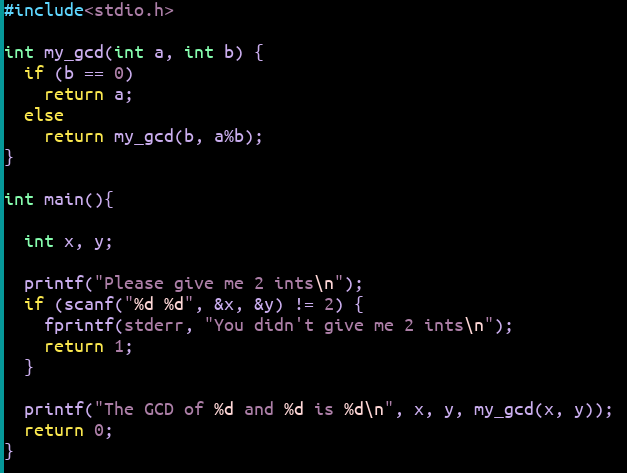
\includegraphics[scale=0.48]{c}\\
\vspace{0.2cm}
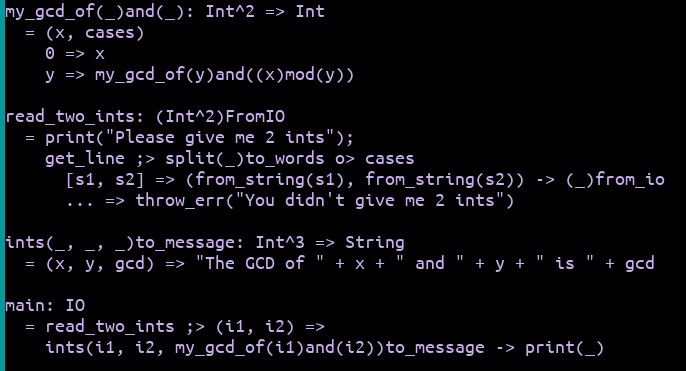
\includegraphics[scale=0.48]{lcases}
\end{center}
\newpage

Μια βασική διαφορά μεταξύ της C και της lcases είναι ότι στην lcases
εμφανίζεται ξεχωριστά το όνομα, ξεχωριστά η έκφραση του τύπου και ξεχωριστά η
έκφραση της ανάθεσης. Αυτό φαίνεται συγκρίνοντας την συνάρτηση "\verb|my_gcd|"
στο C κώδικα με την "\verb|my_gcd_of(_)and(_)|" στον lcases κώδικα.
Συγκεκριμένα, συγκρίνοντας την γραμμή:
\begin{verbatim}
int my_gcd(int a, int b) {
\end{verbatim}
με την γραμμή:
\begin{verbatim}
my_gcd_of(_)and(_): Int^2 => Int
\end{verbatim}
βλέπουμε ότι το γεγονός ότι η συνάρτηση δέχεται δύο ακεραίους και επιστρέφει
έναν ακέραιο γράφεται στην C δίνοντας τον τύπο \textbf{\texttt{int}} σε καθεμία
από τις παραμέτρους και στο αποτέλεσμα, ενώ στην lcases όλα είναι γραμμένα
σε μία ξεχωριστή έκφραση τύπου που δεν έχει ονόματα παραμέτρων ή συνάρτησης.
Επίσης, στην ίδια γραμμή lcases βλέπουμε ότι το όνομα της συνάρτησης έχει
παρένθεση στην μέση, κάτι το οποίο κάνει την συνάρτηση να δέχεται το πρώτο
όρισμα σε εκείνο το σημείο. Η συνάρτηση καλείται αναδρομικά με ορίσματα στις
παρενθέσεις στην γραμμή:
\begin{verbatim}
y => my_gcd_of(y)and((x)mod(y))
\end{verbatim}
όπου μπορούμε επίσης να δούμε ότι η \verb|(_)mod(_)| είναι ορισμένη έτσι ώστε
να δέχεται το πρώτο όρισμά της στην αρχή. Αντίστοιχα, η
\verb|ints(_, _, _)to_message| δέχεται και τα τρία ορίσματά της στην ίδια
παρένθεση στην μέση.

Άλλη μία διαφορά άξια αναφοράς είναι η χρήση της λέξης κλειδιού "cases" στις
γραμμές:
\begin{verbatim}
= (x, cases)
  0 => x
  y => my_gcd_of(y)and((x)mod(y))
\end{verbatim}
αντί της εντολής "if-then" στις γραμμές:
\begin{verbatim}
if (b == 0)
  return a;
else
  return my_gcd(b, a%b);
\end{verbatim}
Χρησιμοποιώντας την λέξη κλειδί "cases" στην θέση της δεύτερης παραμέτρου
υποδεικνύουμε ότι θα πάρουμε περιπτώσεις για τις τιμές της. Αυτό μπορεί να
γίνει για οποιοδήποτε υποσύνολο των παραμέτρων (βλέπε ενότητα
\ref{subsubsec:casessyntaxgr}).

Μια άλλη διαφορά είναι η χρήση του τελεστή πρόσθεσης για την ένωση
συμβολοσειρών και για την αυτόματη μετατροπή των ακεραίων σε συμβολοσειρές
ώστε να συνενωθούν στην γραμμή:
\begin{verbatim}
= (x, y, gcd) => "The GCD of " + x + " and " + y + " is " + gcd
\end{verbatim}
αντί της χρήσης της "printf" με "\%d" στην γραμμή:
\begin{verbatim}
printf("The GCD of %d and %d is %d\n", x, y, my_gcd(x, y));
\end{verbatim}

\newpage
\paragraph{Σύγκριση με \H}
\begin{center}
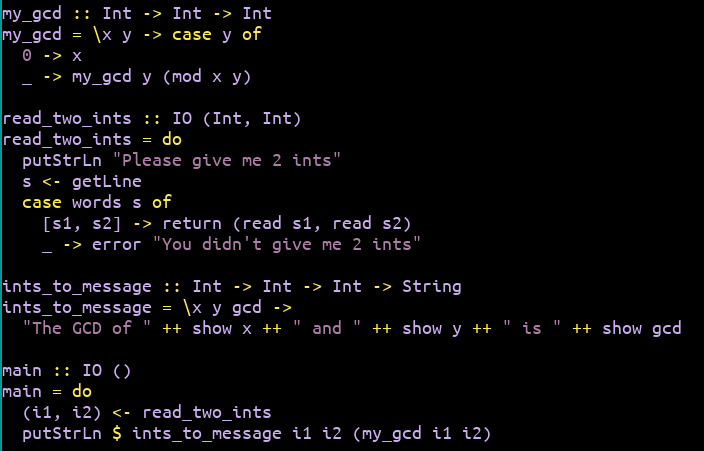
\includegraphics[scale=0.48]{haskell}\\
\vspace{0.2cm}
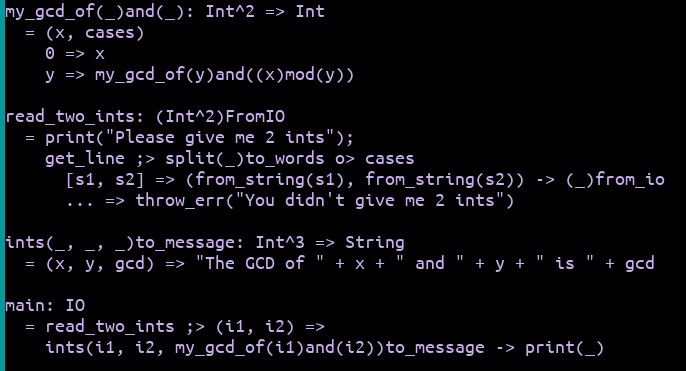
\includegraphics[scale=0.48]{lcases}
\end{center}

Μία σημαντική διαφορά μεταξύ της \H\ και της lcases είναι ότι η εφαρμογή
συνάρτησης στην lcases γίνεται με παρενθέσεις αντί για κενά κάτι το οποίο
επιτρέπει την τοποθέτηση ορισμάτων στην μέση του ονόματος της συνάρτησης.
Αυτό φαίνεται στην σύγκριση της γραμμής:
\begin{verbatim}
my_gcd :: Int -> Int -> Int
\end{verbatim}
με την γραμμή:
\begin{verbatim}
my_gcd_of(_)and(_): Int^2 => Int
\end{verbatim}

Στις ίδιες γραμμές φαίνεται ότι χρησιμοποιούμε έναν τύπο εισόδου και έναν τύπο
εξόδου (όπως στην \H), όμως στην είσοδο έχουμε το γινόμενο των τύπων των
ορισμάτων. Αυτό ίσως φαίνεται περιοριστικό αλλά αντιθέτως είναι πιο γενικό
εφόσον στην lcases είναι εφικτό να δώσουμε ένα υποσύνολο των ορισμάτων
(βάζοντας κάτω παύλα στα υπόλοιπα) και το αποτέλεσμα είναι μία συνάρτηση
που περιμένει τα υπόλοιπα ορίσματα (εκτός αν δώθηκαν όλα), βλέπε ενότητα
\ref{subsubsec:parenfuncappgr}. Στην \H\ τα ορίσματα πρέπει να δωθούν από
αριστερά προς τα δεξιά και μπορούμε να μην δώσουμε τα n δεξιότερα για να
έχουμε αποτέλεσμα μία συνάρτηση που δέχεται αυτά τα n. Ωστόσο, αν για
παράδειγμα θέλουμε να δώσουμε μόνο το δεύτερο πρέπει να χρησιμοποιήσουμε την
"flip" πρώτα. Για πιο περίπλοκα αντίστοιχα πράγματα πρέπει να ορίσουμε
συναρτήσεις παρόμοιες της "flip" κάθε φορά με το χέρι.

Επίσης στις ίδιες γραμμές βλέπουμε την χρήση του τύπου δύναμης \verb|Int^2|
ο οποίος δεν υπάρχει στην \H.

Συγκρίνοντας τις γραμμές:
\begin{verbatim}
my_gcd :: Int -> Int -> Int
my_gcd = \x y -> case y of
\end{verbatim}
με τις γραμμές:
\begin{verbatim}
my_gcd_of(_)and(_): Int^2 => Int
  = (x, cases)
\end{verbatim}
βλέπουμε ότι στην lcases η επισημείωση τύπου και η ανάθεση ομαδοποιούνται για
την αποφυγή της διπλής χρήσης του ονόματος.

Συγκρίνοντας τις γραμμές:
\begin{verbatim}
= (x, cases)
  0 => x
  y => my_gcd_of(y)and((x)mod(y))
\end{verbatim}
με τις γραμμές:
\begin{verbatim}
my_gcd = \x y -> case y of
  0 -> x
  _ -> my_gcd y (mod x y)
\end{verbatim}
βλέπουμε ότι στην lcases χρησιμοποιούμε κατευθείαν την λέξη κλειδί "cases"
στην θέση της παραμέτρου για την οποία θέλουμε να πάρουμε περιπτώσεις χωρίς
να της δίνουμε όνομα. To όνομα δίνεται (αν χρειάζεται) στην γενική/τελευταία
περίπτωση (αν υπάρχει). Η λέξη κλειδί "cases" μπορεί να χρησιμοποιηθεί σε
οποιοδήποτε υποσύνολο των παραμέτρων για να πάρουμε περιπτώσεις για όλες μαζί
ταυτόχρονα (βλέπε \ref{subsubsec:casessyntaxgr}).

Συγκρίνοντας τις γραμμές:
\begin{verbatim}
= print("Please give me 2 ints");
  get_line ;> split(_)to_words o> cases
\end{verbatim}
με τις γραμμές:
\begin{verbatim}
putStrLn "Please give me 2 ints"
s <- getLine
case words s of
\end{verbatim}
βλέπουμε ότι στην lcases δεν χρησιμοποιούμε do notation. Αντί αυτού
χρησιμοποιούμε τους τελεστές περιβάλλοντος "\verb|;|" και "\verb|;>|" οι οποίοι
ισοδυναμούν με τους τελεστές της \H\ "\verb|>>|" και "\verb|>>=|" αντίστοιχα.

Η τελευταία διαφορά που θα αναφέρουμε είναι η χρήση του τελεστή πρόσθεσης για
την ένωση συμβολοσειρών και για την αυτόματη μετατροπή των ακεραίων σε
συμβολοσειρές ώστε να συνενωθούν στην γραμμή:
\begin{verbatim}
= (x, y, gcd) => "The GCD of " + x + " and " + y + " is " + gcd
\end{verbatim}
αντί της χρήσης του τελεστή "\verb|++|" και της "\verb|show|" στην γραμμή:
\begin{verbatim}
"The GCD of " ++ show x ++ " and " ++ show y ++ " is " ++ show gcd
\end{verbatim}

\chapter{Περιγραφή της Γλώσσας: Γενικά}

\section{Δομή Προγράμματος}

Ένα πρόγραμμα lcases αποτελείται από ένα σύνολο ορισμών, παρατσουκλιών τύπων
και θεωρημάτων. Οι ορισμοί είναι χωρισμένοι σε ορισμούς τιμών, ορισμούς τύπων
και ορισμούς προτάσεων τύπων. Τα θεωρήματα είναι αποδεδειγμένες προτάσεις
τύπων. Οι συναρτήσεις καθώς και οι "δράσεις περιβάλλοντος" θεωρούνται επίσης
τιμές.  Ο ορισμός της τιμής "main" καθορίζει την συμπεριφορά του προγράμματος.

\paragraph{Παράδειγμα Προγράμματος: Ευκλείδιος Αλγόριθμος}
\begin{verbatim}
gcd_of(_)and(_): Int^2 => Int
  = (x, cases)
    0 => x
    y => gcd_of(y)and((x)mod(y))

read_two_ints: (Int^2)FromIO
  = print("Please give me 2 ints");
    get_line ;> split(_)to_words o> cases
      [x, y] => (from_string(x), from_string(y)) -> (_)from_io
      ... => throw_err("You didn't give me 2 ints")

tuple_type NumsAndGcd
value (x, y, gcd):Int^3

nag(_)to_message: NumsAndGcd => String
  = nag => "The GCD of " + nag.x + " and " + nag.y + " is " + nag.gcd

main: IO
  = read_two_ints ;> (i1, i2) =>
    (i1, i2, gcd_of(i1)and(i2)) -> nag(_)to_message -> print(_)
\end{verbatim}

\newpage
\section{Λέξεις κλειδιά}

Οι λέξεις κλειδιά της lcases είναι:
\begin{verbatim}
cases all where tuple_type value or_type values
type_proposition needed equivalent type_theorem proof
\end{verbatim}
Η χρήση της κάθεμίας περιγράφεται στην αντίστοιχη ενότητα του παρακάτω πίνακα:

\begin{center}
\centering
\begin{tabular}{ |c|c| }
\hline
Keyword & Section
\\
\hline
\hline
\verb|cases| & \ref{subsubsec:casessyntaxgr} Εκφράσεις Συναρτήσεων "cases"
\\
\hline
\verb|all where| & \ref{subsec:valdefswheregr}
Ορισμοί Τιμών και Εκφράσεις "where"
\\
\hline

\begin{tabular}{@{}c@{}}
\verb|tuple_type value or_type|
\\
\verb|values type_nickname|
\end{tabular}
&
\ref{subsec:typesgr} Τύποι
\\
\hline
\begin{tabular}{@{}c@{}}
\verb|type_proposition needed|\\
\verb|equivalent type_theorem proof|
\end{tabular}
&
\ref{subsec:typelogicgr} Λογική Τύπων
\\
\hline
\end{tabular}

\end{center}
Οι λέξεις κλειδιά "\verb|cases|" και "\verb|where|" είναι επίσης κατοχυρωμένες
λέξεις. Επομένως, παρόλο που μπορούν να παραχθούν από την γραμματική τον
ονομάτων, δεν μπορούν να χρησιμοποιηθούν σαν ονόματα.

\chapter{Περιγραφή της Γλώσσας: Τιμές}

\section{Βασικές Εκφράσεις}

\subsection{Σταθερές και Ονόματα}

\paragraph{Σταθερές}
\begin{itemize}

\item \textit{Παραδείγματα}
\begin{verbatim}
1  2  17  42  -100
1.62  2.72  3.14  -1234.567
'a'  'b'  'c'  'x'  'y'  'z'  '.'  ','  '\n'
"Hello World!"  "What's up, doc?"  "Alrighty then!"
\end{verbatim}

\item \textit{Περιγραφή}

Υπάρχουν σταθερές για τους τέσσερις βασικούς τύπους:
\texttt{Int, Real, Char, String}.

\end{itemize}

\paragraph{Ονόματα}
\begin{itemize}

\item \textit{Παραδείγματα}
\begin{verbatim}
x y z
a1 a2 a3
(_)mod(_)
apply(_)to_all_in(_)
\end{verbatim}

\item \textit{Περιγραφή}

Τα ονόματα χρησιμοποιούνται για τιμές και παραμέτρους. Ένα όνομα τιμής
χρησιμοποιείται στον ορισμό της τιμής και στις εκφράσεις που χρησιμοποιούν
αυτή την τιμή. Ένα όνομα παραμέτρου χρησιμοποιείται στο σώμα της συνάρτησης
της οποίας είναι παράμετρος.
\\\\
Ένα όνομα ξεκινάει με μικρό αγγλικό γράμμα και μπορεί να ακολουθηθεί
από μικρά αγγλικά γράμματα ή κάτω παύλα και/ή να έχει ένα ψηφίο στο τέλος.
Είναι επίσης δυνατόν να υπάρχουν κάτω παύλες μέσα σε παρένθεση πριν, μετά ή
και κάπου στην μέση του ονόματος (η χρήση τους περιγράφεται στην ενότητα
"Εφαρμογή Συνάρτησης με Παρενθέσεις" \ref{subsubsec:parenfuncappgr})

\end{itemize}

\newpage
\subsection{Παρενθέσεις, Πλειάδες και Λίστες}

\paragraph{Παρενθέσεις}

\begin{itemize}

\item \textit{Παραδείγματα}
\begin{verbatim}
(1 + 2)
(((1 + 2) * 3)^4)
(n => 3*n + 1)
(get_line ;> line => print("Line is: " + line))
\end{verbatim}

\item \textit{Περιγραφή}

Μια έκφραση μπαίνει σε παρένθεση για να της δοθεί προτεραιότητα ή να απομονωθεί
σε μια μεγαλύτερη έκφραση (τελεστών).  Οι εκφράσεις μέσα σε παρένθεση είναι
εκφράσεις τελεστών ή εκφράσεις συναρτήσεων.
\\\\
Οι εκφράσεις μέσα σε παρένθεση δεν μπορούν να επεκταθούν σε περισσότερες από
μία γραμμές. Για εκφράσεις μεγαλύτερες από μία γραμμή, πρέπει να οριστεί νέα
τιμή.

\end{itemize}

\paragraph{Πλειάδες}

\begin{itemize}

\item \textit{Παραδείγματα}
\begin{verbatim}
(1, "What's up, doc?")
(2, "Alrighty then!", 3.14)
(x, y, z, w)
(1, my_function, (x, y, z) => sqrt(x^2 + y^2 + z^2))
\end{verbatim}

\item \textit{Περιγραφή}

Οι πλειάδες χρησιμοποιούνται για να ομαδοποιήσουν πολλές τιμές (που μπορούν
να έχουν διαφορετικό τύπο) σε μία. Ο τύπος της πλειάδας είναι είτε το γινόμενο
των τύπων των στοιχείων της είτε ένας ορισμένος τύπος \verb|tuple_type|
που είναι ισοδύναμος με τον προαναφερθέντα τύπο γινομένου.
Για παράδειγμα, ο τύπος της δεύτερης πλειάδας στα παραδείγματα θα μπορούσε να
είναι:
\begin{verbatim}
Int x String x Real
\end{verbatim}
ή:
\begin{verbatim}
MyType
\end{verbatim}
υποθέτοντας ότι ο τύπος "\verb|MyType|" έχει ορισμό παρόμοιο με τον παρακάτω:
\begin{verbatim}
tuple_type MyType
value (my_int, my_string, my_real) : Int x String x Real
\end{verbatim}

\newpage
\item \textit{Πλειάδες με κενά στοιχεία}
\\\\
\textbf{Παραδείγματα}
\begin{verbatim}
(42, _)
(_, 3.14, _)
(_, _, "Hello from 3rd field")
\end{verbatim}

\textbf{Περιγραφή}
\\\\
Είναι εφικτό να μείνουν κενά κάποια στοιχεία μια πλειάδας χρησιμοποιώντας
κάτω παύλα στην θέση τους. Η χρήση κενών στοιχείων δημιουργεί μία συνάρτηση
που περιμένει τα κενά στοιχεία σαν ορίσματα για να επιστρέψει την συνολική
πλειάδα. Αυτό φαίνεται καλύτερα από τους τύπους των παραπάνω παραδειγμάτων:
\begin{verbatim}
(42, _) : T1 => Int x T1
(_, 3.14, _) : T1 x T2 => T1 x Real x T2
(_, _, "Hello from 3rd field") : T1 x T2 => T1 x T2 x String
\end{verbatim}
Ένα παράδειγμα σε μεγαλύτερη έκφραση είναι το παρακάτω:
\begin{verbatim}
questions : ListOf(String)s
  = ["the Ultimate Question of Life", "the Universe", "Everything"]

answers_to : ListOf(String)s
  = apply("The answer to " + _)to_all_in(questions)
\end{verbatim}

\begin{verbatim}
>> apply((42, _))to_all_in(answers_to)
  : ListOf(Int x String)s
  ==> [ (42, "The answer to the Ultimate Question of Life")
      , (42, "The answer to the Universe")
      , (42, "The answer to Everything")
      ]
\end{verbatim}

\end{itemize}

\paragraph{Λίστες}

\begin{itemize}

\item \textit{Παραδείγματα}
\begin{verbatim}
[1, 2, 17, 42, -100]
[1.62, 2.72, 3.14, -1234.567]
["Hello World!", "What's up, doc?", "Alrighty then!"]
[x => x + 1, x => x + 2, x => x + 3]
[x, y, z, w]
\end{verbatim}

\item \textit{Περιγραφή}

Οι λίστες χρησιμοποιούνται για την ομαδοποίηση πολλών τιμών του ίδιου τύπου σε
μία.  Ο τύπος της λίστας είναι \verb|ListOf(T1)s| όπου \verb|T1| είναι ο τύπος
κάθε στοιχείου της λίστας.  Επομένως, οι τύποι των τεσσάρων πρώτων
παραδειγμάτων είναι:
\begin{verbatim}
ListOf(Int)s
ListOf(Real)s
ListOf(String)s
(@A)And(Int)Add_To(@B) --> ListOf(@A => @B)s
\end{verbatim}

\end{itemize}

\subsection{Εφαρμογή Συνάρτησης με Παρενθέσεις}
\label{subsubsec:parenfuncappgr}

\begin{itemize}
\item \textit{Παραδείγματα}

\begin{verbatim}
f(x)
f(x, y, z)
(x)to_string
apply(f)to_all_in(l)
\end{verbatim}

\item \textit{Περιγραφή}

Η εφαρμογή συνάρτησης στην lcases μπορεί να γίνει με πολλούς τρόπους.  Σε αυτή
την ενότητα περιγράφονται οι τρόποι με τους οποίους γίνεται εφαρμογή συνάρτησης
με παρενθέσεις.
\\\\
Στα πρώτα δύο παραδείγματα έχουμε την συνηθισμένη μαθηματική εφαρμογή
συνάρτησης όπου τα ορίσματα είναι μετά το όνομα της συνάρτησης.
\\\\
Στην lcases επεκτείνεται αυτή η ιδέα επιτρέποντας να υπάρχουν ορίσματα πριν
ή/και κάπου μέσα στο όνομα της συνάρτησης (παραδείγματα 3 και 4). Αυτό μπορεί
να γίνει μόνο αν η συνάρτηση είναι ορισμένη με τις αντίστοιχες θέσεις όπου
τοποθετούνται τα ορίσματα. Για παράδειγμα, ο ορισμός για την
"\verb|apply(_)to_all_in(_)|" ξεκινάει ως εξής:
\begin{verbatim}
apply(_)to_all_in(_) : (T1 => T2) x ListOf(T1)s => ListOf(T2)s
  = <...definition>
\end{verbatim}
Το όνομα της συνάρτησης συμπεριλαμβάνει τις παρενθέσεις με τις κάτω παύλες οι
οποίες λειτουργούν ως θέσεις για ορίσματα.  Αυτό είναι πολύ χρήσιμο για τον
ορισμό συναρτήσεων όπου τα ορίσματα μέσα ή πριν την συνάρτηση κάνουν την
εφαρμογή της συνάρτησης να φαίνεται και να ακούγεται περισσότερο σαν φυσική
γλώσσα.

\item \textit{Κενά Ορίσματα σε Εφαρμογή Συνάρτησης με Παρενθέσεις}
\\\\
Είναι εφικτό να δοθεί σε μία συνάρτηση ένα υποσύνολο των ορισμάτων της βάζοντας
κάτω παύλα στα υπόλοιπα ορίσματα. Μια τέτοια έκφραση είναι μια συνάρτηση που
περιμένει τα ορίσματα που λείπουν για να επιστρέψει το τελικό αποτέλεσμα.
Παραδείγματα:
\begin{verbatim}
f(_, _, _) : Char x Int x Real => String
c, i, r : Char, Int, Real

f(c, i, r) : String

f(_, i, r) : Char => String
f(c, _, r) : Int => String
f(c, i, _) : Real => String

f(c, _, _) : Int x Real => String
f(_, i, _) : Char x Real => String
f(_, _, r) : Char x Int => String
\end{verbatim}

\end{itemize}

\newpage
\subsection{Συναρτήσεις Προθήματος και Επιθήματος}

\paragraph{Συναρτήσεις Προθήματος}

\begin{itemize}

\item \textit{Παραδείγματα}
\begin{verbatim}
the_value:1
error:e
result:r
apply(the_value:_)to_all_in(_)
\end{verbatim}

\item \textit{Περιγραφή}

Οι συναρτήσεις προθήματος δημιουργούνται αυτόματα από ορισμούς τύπων
\verb|or_type|. Είναι συναρτήσεις που μετατρέπουν μία τιμή ενός συγκεκριμένου
τύπου σε μια τιμή που είναι περίπτωση ενός \verb|or_type| και περιέχει
τιμές του προαναφερθέντα τύπου εσωτερικά.
Π.χ. για το πρώτο απ'τα παραπάνω παραδείγματα έχουμε:
\begin{verbatim}
1 : Int
the_value:1 : Possibly(Int)
\end{verbatim}
Όπου η συνάρτηση \verb|the_value:_| δημιουργήθηκε αυτόματα από το ορισμού
του τύπου \verb|Possibly(_)|:
\begin{verbatim}
or_type Possibly(T1)
values the_value:T1 | no_value
\end{verbatim}
Και έχει τύπο \verb|T1 => Possibly(T1)|.
\\\\
Οι συναρτήσεις αυτές αποκαλούνται συναρτήσεις προθήματος γιατί τοποθετούνται
πριν από το όρισμά τους. Μπορούν όμως να χρησιμοποιηθούν και σαν ορίσματα άλλων
συναρτήσεων τοποθετώντας μία κάτω παύλα στο όρισμά τους.  Αυτό φαίνεται
στο τελευταίο παράδειγμα, όπου η συνάρτηση \verb|the_value:_| είναι όρισμα της
συνάρτησης \verb|apply(_)to_all_in(_)|.

\end{itemize}

\newpage
\paragraph{Συναρτήσεις Επιθήματος}

\begin{itemize}

\item \textit{Παραδείγματα}
\begin{verbatim}
name.first_name
list.head
date.year
tuple.1st
apply(_.1st)to_all_in(_)
\end{verbatim}

\item \textit{Περιγραφή}

Οι συναρτήσεις επιθήματος δημιουργούνται αυτόματα από ορισμούς τύπων
\verb|tuple_type|. Είναι συναρτήσεις που δέχονται μία τιμή κάποιου
\verb|tuple_type| τύπου και επιστρέφουν κάποιο στοιχείο της τιμής
(ήτοι συναρτήσεις προβολής).
Π.χ. για το πρώτο από τα παραπάνω παραδείγματα έχουμε:
\begin{verbatim}
name : Name
name.first_name : String
\end{verbatim}
Όπου η συνάρτηση \verb|_.first_name| δημιουργήθηκε αυτόματα από τον ορισμό
του τύπου \verb|Name|:
\begin{verbatim}
tuple_type Name
value (first_name, last_name) : String^2
\end{verbatim}
Και έχει τύπο \verb|Name => String|.
\\\\
Υπάρχουν επίσης οι παρακάτω ειδικές συναρτήσεις προβολής που λειτουργούν σε
όλες τις πλειάδες που είναι τύπου γινομένου:
"\verb|_.1st|", "\verb|_.2nd|", "\verb|_.3rd|", "\verb|_.4th|", "\verb|_.5th|".
Για το τέταρτο παράδειγμα παραπάνω, υποθέτοντας:
\begin{verbatim}
tuple : Int x String
\end{verbatim}
Έχουμε:
\begin{verbatim}
tuple.1st : Int
\end{verbatim}
Οι γενικοί τύποι των συναρτήσεων αυτών είναι:
\begin{verbatim}
_.1st : (@A)Is(@B)s_1st --> @B => @A
_.2nd : (@A)Is(@B)s_2nd --> @B => @A
...
\end{verbatim}
Οι συναρτήσεις αυτές αποκαλούνται συναρτήσεις επιθήματος γιατί τοποθετούνται
μετά από το όρισμά τους. Μπορούν όμως να χρησιμοποιηθούν και σαν ορίσματα άλλων
συναρτήσεων τοποθετώντας μία κάτω παύλα στο όρισμά τους.  Αυτό απεικονίζεται
στο τελευταίο παράδειγμα, όπου η συνάρτηση \verb|_.1st| είναι όρισμα της
συνάρτησης \verb|apply(_)to_all_in(_)|.
\\\\
Υπάρχει επίσης μία ειδική συνάρτηση επιθήματος που ονομάζεται "\verb|_.change|"
και περιγράφεται στην επόμενη παράγραφο.

\end{itemize}

\paragraph{The ".change" Function}

\begin{itemize}

\item \textit{Παραδείγματα}

\begin{verbatim}
state.change{counter = counter + 1}
tuple.change{1st = 42, 3rd = 17}
point.change{x = 1.62, y = 2.72, z = 3.14}
apply(_.change{1st = 1st + 1})to_all_in(_)
x.change{1st = _, 3rd = _}
\end{verbatim}

\item \textit{Περιγραφή}
\\\\
Οι συνάρτηση "\verb|_.change|" είναι μία ειδική συνάρτηση επιθήματος που
λειτουργεί σε όλες τις πλειάδες. Επιστρέφει μία νέα πλειάδα η οποία είναι ίδια
με την αρχική εκτός από κάποια στοιχεία που αλλάζουν. Το ποια στοιχεία αλλάζουν
και σε ποια νέα τιμή προσδιορίζεται μέσα σε άγκιστρα μετά το "\verb|.change|".
Τα παρακάτω ειδικά ονόματα μπορούν επίσης να χρησιμοποιηθούν για αναφορά στα
στοιχεία μιας πλειάδας τύπου γινομένου: "\verb|1st|", "\verb|2nd|",
"\verb|3rd|", "\verb|4th|", "\verb|5th|" (παραδείγματα 2, 4 και 5). Αν η
πλειάδα είναι κάποιου \verb|tuple_type| τύπου, χρησιμοποιούνται τα ονόματα των
στοιχείων που ορίστηκαν στον ορισμό του τύπου (παραδείγματα 1 και 3).
Επομένως, έχουμε υποθέσει τα παρακάτω (ή παρόμοια) ώστε τα παραδείγματα να
έχουν ορθούς τύπους:

\begin{verbatim}
tuple_type MyStateType
value (..., counter, ...) : ... x Int x ...

state : MyStateType


tuple : Int x SomeType x Int (x ...)


tuple_type Point
value (x, y, z) : Real^3

point : Point


apply(_.change{1st = 1st + 1})to_all_in(_)
  : (@A)And(Int)AddTo(@A), (@A)Is(@B)s_1st --> ListOf(@B)s => ListOf(@B)s


x : Int x Real x String
x.change{1st = _, 3rd = _} : Int x String => Int x Real x String
\end{verbatim}

Οι αλλαγές στοιχείων έχουν την μορφή: "\verb|στοιχείο = <έκφραση νέας τιμής>|"
και χωρίζονται από κόμματα. Οι τιμές της αρχικής πλειάδας μπορούν να
χρησιμοποιηθούν στις εκφράσεις των νέων τιμών και χρησιμοποιούνται τα ονόματα
των στοιχείων για την αναφορά σε αυτές (παραδείγματα 1 και 4). Επίσης, μπορούν
να χρησιμοποιηθούν κάτω παύλες στις νέες τιμές. Αυτό κάνει την έκφραση μία
συνάρτηση που περιμένει τις κενές τιμές ως ορίσματα (τελευταίο παράδειγμα).

\end{itemize}

\section{Τελεστές}

\subsection{Τελεστές Εφαρμογής Συνάρτησης και Σύνθεσης Συναρτήσεων}

\paragraph{Τελεστές Εφαρμογής Συνάρτησης}

\begin{center}
\begin{tabular}{ |c|c|c| }
\hline
Τελεστής & Τύπος
\\
\hline
\hline
\verb|->| & \verb| T1 x (T1 => T2) => T2|
\\
\hline
\verb|<-| & \verb| (T1 => T2) x T1 => T2|
\\
\hline
\end{tabular}
\end{center}
Οι τελεστές εφαρμογής συνάρτησης "\verb|->|" και "\verb|<-|" είναι ένας
διαφορετικός τρόπος εφαρμογής συνάρτησης από την εφαρμογή με παρένθεση.  Είναι
φτιαγμένοι ώστε να μοιάζουν με βέλη από το όρισμα προς την συνάρτηση. Οι
τελεστές αυτοί είναι πολύ χρήσιμοι για την εφαρμογή πολλών συναρτήσεων στην
σειρά χωρίς να χρειάζεται ο αντίστοιχος αριθμός ανοίγματος και κλεισίματος
παρενθέσεων. Για παράδειγμα, υποθέτοντας ότι έχουμε τις παρακάτω συναρτήσεις με
την συμπεριφορά που υπονοείται από τα ονόματα και τους τύπους τους:
\begin{verbatim}
apply(_)to_all_in(_) : (T1 => T2) x ListOf(T1)s => ListOf(T2)s
str_len(_) : String => Int
filter(_)with(_) : ListOf(T1)s x (T1 => Bool) => ListOf(T1)s
(_)is_odd : Int => Bool
sum_ints(_) : ListOf(Int)s => Int
\end{verbatim}
Και μια λίστα από συμβολοσειρές:
\begin{verbatim}
strings : ListOf(String)s
\end{verbatim}
Ο παρακάτω είναι ένας απλός τρόπος να πάρουμε το συνολικό αριθμό χαρακτήρων
σε όλες τις συμβολοσειρές που έχουν περιττό μήκος:
\begin{verbatim}
chars_in_odd_length_strings : Int
  = apply(str_len(_))to_all_in(strings) -> filter(_)with((_)is_odd) -> sum_ints(_)
\end{verbatim}
Αυτό μπορεί να γίνει ισοδύναμα χρησιμοποιώντας τον τελεστή της αντίθετης
κατεύθυνσης:
\begin{verbatim}
chars_in_odd_length_strings : Int
  = sum_ints(_) <- filter(_)with((_)is_odd) <- apply(str_len(_))to_all_in(strings)

\end{verbatim}

\newpage

\paragraph{Τελεστές Σύνθεσης Συναρτήσεων}
\begin{center}
\begin{tabular}{ |c|c|c| }
\hline
Τελεστής & Τύπος
\\
\hline
\hline
\verb|o>| & \verb|(T1 => T2) x (T2 => T3) => (T1 => T3)|
\\
\hline
\verb|<o| & \verb|(T2 => T3) x (T1 => T2) => (T1 => T3)|
\\
\hline
\end{tabular}
\end{center}
Οι τελεστές σύνθεσης συναρτήσεων "\verb|o>|" και "\verb|<o|" χρησιμοποιούνται
για την σύνθεση συναρτήσεων, ο καθένας στην αντίστοιχη κατεύθυνση. Η χρήση του
γράμματος '\verb|o|' αποσκοπεί στην ομοιότητα με το σύμβολο σύνθεσης
συναρτήσεων στα μαθηματικά '\(\circ\)' και τα σύμβολα '\verb|>|', '\verb|<|'
χρησιμοποιούνται ώστε οι τελεστές να "δείχνουν" από την συνάρτηση που θα
εφαρμοστεί πρώτη στην συνάρτηση που θα εφαρμοστεί δεύτερη. Ένα ωραίο
παράδειγμα χρήσης των τελεστών σύνθεσης συναρτήσεων είναι το παρακάτω.
Υποθέτοντας ότι έχουμε τις παρακάτω συναρτήσεις με την συμπεριφορά που
υπονοείται από τα ονόματα και τους τύπους τους:
\begin{verbatim}
split(_)to_words : String => ListOf(String)s
apply(_)to_all_in(_) : (T1 => T2) x ListOf(T1)s => ListOf(T2)s
reverse_str(_) : String => String
merge_words(_) : ListOf(String)s => String
\end{verbatim}
Μπορούμε να αντιστρέψουμε όλες τις λέξεις σε μια συμβολοσειρά ως εξής:
\begin{verbatim}
reverse_words_in(_) : String => String
  = split(_)to_words o> apply(reverse_str(_))to_all_in(_) o> merge_words(_)
\end{verbatim}
Αυτό μπορεί να γίνει ισοδύναμα χρησιμοποιώντας τον τελεστή της αντίθετης
κατεύθυνσης:
\begin{verbatim}
reverse_words_in(_) : String => String
  = merge_words(_) <o apply(reverse_str(_))to_all_in(_) <o split(_)to_words
\end{verbatim}

\newpage
\subsection{Αριθμητικοί, Σχεσιακοί και Λογικοί Τελεστές}

\paragraph{Αριθμητικοί Τελεστές}
\begin{center}
\begin{tabular}{ |c|c|c| }
\hline
Τελεστής & Τύπος
\\
\hline
\hline
\verb|^| & \verb|(@A)To_The(@B)Is(@C) --> @A x @B => @C|
\\
\hline
\verb|*| & \verb|(@A)And(@B)Multiply_To(@C) --> @A x @B => @C|
\\
\hline
\verb|/| & \verb|(@A)Divided_By(@B)Is(@C) --> @A x @B => @C|
\\
\hline
\verb|+| & \verb|(@A)And(@B)Add_To(@C) --> @A x @B => @C|
\\
\hline
\verb|-| & \verb|(@A)Minus(@B)Is(@C) --> @A x @B => @C|
\\
\hline
\end{tabular}
\end{center}
Οι συνηθισμένοι αριθμητικοί τελεστές λειτουργούν όπως στα μαθηματικά και στις
άλλες γλώσσες προγραμματισμού για τους συνηθισμένους τύπους. Ωστόσο, είναι
γενικευμένοι. Τα παρακάτω παραδείγματα δείχνουν την γενικότητά τους:
\begin{verbatim}
>> 1 + 1
: Int
==> 2
>> 1 + 3.14
: Real
==> 4.14
>> 'a' + 'b'
: String
==> "ab"
>> 'w' + "ord"
: String
==> "word"
>> "Hello " + "World!"
: String
==> "Hello World!"
>> 5 * 'a'
: String
==> "aaaaa"
>> 5 * "hi"
: String
==> "hihihihihi"
>> "1,2,3" - ','
: String
==> "123"
\end{verbatim}
Ας αναλύσουμε περισσότερο το παράδειγμα της πρόσθεσης.  Ο τύπος μπορεί να
διαβαστεί ως εξής: ο τελεστής '\verb|+|' έχει τύπο \verb|@A x @B => @C|,
δεδομένου ότι ισχύει η πρόταση \verb|(@A)And(@B)Add_To(@C)|.
Η αλήθεια της προτάσεως σημαίνει ότι η πρόσθεση έχει οριστεί για αυτούς τους
τρεις τύπους.
Επομένως, από τα παραπάνω παραδείγματα μπορούμε να συμπεράνουμε ότι οι
παρακάτω προτάσεις είναι αληθείς:
\begin{verbatim}
(Int)And(Int)Add_To(Int)
(Int)And(Real)Add_To(Real)
(Char)And(Char)Add_To(String)
(Char)And(String)Add_To(String)
(Int)And(Char)Multiply_To(String)
(Int)And(String)Multiply_To(String)
(String)Minus(Char)Is(String)
\end{verbatim}
Αυτό επιτρέπει την χρήση των γνώριμων αριθμητικών τελεστών σε τύπους οι
οποίοι δεν είναι απαραίτητα αριθμοί αλλά είναι αρκετά προφανές το τι
συμπεριφορά θα πρέπει να έχουν για αυτούς τους τύπους. Επιπλέον, οι συμπεριφορά
τους μπορεί να οριστεί από τον χρήστη για τύπους ορισμένους επίσης από το
χρήστη!

\paragraph{Σχεσιακοί, Λογικοί και bitwise τελεστές}

\begin{center}
\begin{tabular}{ |c|c|c| }
\hline
Τελεστής & Τύπος
\\
\hline
\hline
\verb|==| & \verb|(@A)And(@B)Can_Be_Equal --> @A x @B => Bool|
\\
\hline
\verb|!=| & \verb|(@A)And(@B)Can_Be_Unequal --> @A x @B => Bool|
\\
\hline
\verb|>| & \verb|(@A)Can_Be_Greater_Than(@B) --> @A x @B => Bool|
\\
\hline
\verb|<| & \verb|(@A)Can_Be_Less_Than(@B) --> @A x @B => Bool|
\\
\hline
\verb|>=| & \verb|(@A)Can_Be_Gr_Or_Eq_To(@B) --> @A x @B => Bool|
\\
\hline
\verb|<=| & \verb|(@A)Can_Be_Le_Or_Eq_To(@B) --> @A x @B => Bool|
\\
\hline
\verb|&| & \verb|(@A)Has_And --> @A^2 => @A|
\\
\hline
\texttt{|} & \verb|(@A)Has_Or --> @A^2 => @A|
\\
\hline
\end{tabular}
\end{center}
Οι σχεσιακοί τελεστές είναι επίσης γενικευμένοι. Ο βασικός λόγος για την
γενίκευσή τους είναι η σύγκριση αριθμών διαφορετικών τύπων όπως φαίνεται στο
παρακάτω παράδειγμα:
\begin{verbatim}
>> 1
  : Int
  ==> 1
>> 1.1
  : Real
  ==> 1.1
>> 1.1 == 1
  : Bool
  ==> false
>> 1.0 == 1
  : Bool
  ==> true
\end{verbatim}
Για να λειτουργήσει το παράδειγμα πρέπει να μπορούμε να συγκρίνουμε ακεραίους
με πραγματικούς.  Αντίστοιχα, όλοι οι σχεσιακοί τελεστές πρέπει να μπορούν να
λειτουργήσουν με ορίσματα διαφορετικών τύπων.
\\\\
Το λογικό "και" και το bitwise "και" έχουν συγχωνευτεί σε ένα γενικό
τελεστή "και" (\verb|&|). Το ίδιο ισχύει και για τον τελεστή "ή" (\texttt{|}).

\newpage
\subsection{Τελεστές Δράσεων σε Περιβάλλον}

\begin{center}
\begin{tabular}{ |c|c|c| }
\hline
Τελεστής & Τύπος
\\
\hline
\hline
\verb|;>| & \verb|(@E(_))Has_Use --> @E(T1) x (T1 => @E(T2)) => @E(T2)|
\\
\hline
\verb|;| & \verb|(@E(_))Has_Then --> @E(T1) x @E(T2) => @E(T2)|
\\
\hline
\end{tabular}
\end{center}

\paragraph{Απλό Παράδειγμα Προγράμματος}
\begin{verbatim}
main: (EmptyVal)FromIO
  = print_string("I'll repeat the line") ; get_line ;> print_string(_)
\end{verbatim}
Στο παραπάνω παράδειγμα φαίνεται η χρήση των τελεστών δράσεων σε περιβάλλον με
τον τύπο περιβάλλοντος \verb|(_)FromIO|, ο οποίος είναι ο τύπος με τον οποίο
γίνεται είσοδος/έξοδος στην lcases. Το πως ακριβώς γίνεται αυτό μπορεί να φανεί
αν ρίξουμε μια ματιά στους τύπους (όπως πάντα!):
\begin{verbatim}
print_string(_): String => (EmptyVal)FromIO
print_string("I'll repeat the line"): (EmptyVal)FromIO
get_line: (String)FromIO

\end{verbatim}
Για τον τελεστή "έπειτα" έχουμε:
\verb|; : (@E(_))Has_Then --> @E(T1) x @E(T2) => @E(T2)|
\\\\
Στην παρακάτω έκφραση:
\verb|print_string("I'll repeat the line") ; get_line|
\\
ο τελεστής "έπειτα" έχει τύπο:
\verb|(EmptyVal)FromIO x (String)FromIO => Κάποιο Τύπο Τ|
\\\\
Ο μόνος τρόπος να ταιριάξουν οι τύποι είναι αν:
\\
\verb|  @E(_) = (_)FromIO, T1 = EmptyVal, T2 = String και T = (String)FromIO|
\\
Και λειτουργεί γιατί: \verb|((_)FromIO)Has_Then|
\\\\
Για την συνολική έκφραση έχουμε:
\begin{verbatim}
print_string("I'll repeat the line") ; get_line
  : (String)FromIO

\end{verbatim}
Για τον τελεστή "χρησιμοποίησε" έχουμε:
\\
\verb|;> : (@E(_))Has_Use --> @E(T1) x (T1 => @E(T2)) => @E(T2)|
\\\\
Στην παρακάτω έκφραση:
\\
\verb|print_string("I'll repeat the line") ; get_line ;> print_string(_)|
\\
ο τελεστής "χρησιμοποίησε" έχει τύπο:
\\
\verb|(String)FromIO x (String => (EmptyVal)FromIO) => Κάποιο Τύπο Τ|
\\\\
Ο μόνος τρόπος να ταιριάξουν οι τύποι είναι αν:
\\
\verb|  @E(_) = (_)FromIO, T1 = String, T2 = EmptyVal και Τ = (EmptyVal)FromIO|
\\
Και λειτουργεί γιατί: \verb|((_)FromIO)Has_Use|
\\\\
Για την συνολική έκφραση έχουμε:
\begin{verbatim}
print_string("I'll repeat the line") ; get_line ;> print_string(_)
  : (EmptyVal)FromIO
\end{verbatim}

\newpage
\paragraph{Ακόμα ένα Παράδειγμα Προγράμματος}
\begin{verbatim}
main: (EmptyVal)FromIO
  = print_string("Hello! What's your name?") ; get_line ;> name =>
    print_string("And how old are you?") ; get_line ;> age =>
    print_string("Oh! You don't look " + age + " " + name + "!")

print_string(_): String => (EmptyVal)FromIO

print_string("Hello! What's your name?") : (EmptyVal)FromIO

print_string("Hello! What's your name?"); get_line
  : (String)FromIO

print_string("And how old are you?"); get_line
  : (String)FromIO

print_string("Oh! You don't look " + age + " " + name + "!")
  : (EmptyVal)FromIO

age => print_string("Oh! You don't look " + age + " " + name + "!")
  : String => (EmptyVal)FromIO

print_string("And how old are you?") ; get_line ;> age =>
print_string("Oh! You don't look " + age + " " + name + "!")
  : (EmptyVal)FromIO

name =>
print_string("And how old are you?") ; get_line ;> age =>
print_string("Oh! You don't look " + age + " " + name + "!")
  : String => (EmptyVal)FromIO

print_string("Hello! What's your name?") ; get_line ;> name =>
print_string("And how old are you?") ; get_line ;> age =>
print_string("Oh! You don't look " + age + " " + name + "!")
  : (EmptyVal)FromIO
\end{verbatim}

\paragraph{Περιγραφή}\pend
Οι τελεστές δράσεων σε περιβάλλον χρησιμοποιούνται για να συνδυάσουν τιμές που
είναι δράσεις σε περιβάλλον σε τιμές που είναι πιο περίπλοκες δράσεις σε
περιβάλλον. Οι τύποι περιβάλλοντος είναι συναρτήσεις τύπων που δέχονται ένα
τύπο σαν όρισμα και δημιουργούν έναν άλλον τύπο (όπως ο τύπος
\verb|ListOf(_)s|). Οι τελεστές "έπειτα" (\verb|;|) και "χρησιμοποίησε"
(\verb|;>|) είναι ορισμένοι για τους τύπους περιβάλλοντος. Μια τιμή τύπου
\verb|@E(T1)| όπου ο \verb|@E(_)| είναι τύπος περιβάλλοντος κάνει μια δράση
στο περιβάλλον \verb|@E(_)| και δημιουργεί μια τιμή τύπου \verb|T1|. Αυτή η
δράση μπορεί να συνδυαστεί με τον τελεστή "έπειτα" με μία άλλη ώστε να γίνει
η πρώτη και έπειτα η δεύτερη. Αντίστοιχα, με τον τελεστή "χρησιμοποίησε"
οι τιμή που δημιουργήθηκε από την πρώτη δράση, μπορεί να χρησιμοποιηθεί σαν
όρισμα σε συνάρτηση που επιστρέφει μια δεύτερη δράση.

\newpage
\subsection{Εκφράσεις Τελεστών}

\begin{itemize}
\item \textit{Παραδείγματα}
\begin{verbatim}
1 + 2
1 + x * 3^y
"Hello " + "World!"
x -> f -> g
f o> g o> h
x == y
x >= y - z & x < 2 * y
get_line ; get_line ;> line => print("Second line: " + line)
2 * _
_ - 1
"Hello " + "it's me, " + _
"Hi, I am " + _ + " and I am " + _ + " years old"
\end{verbatim}

\item \textit{Περιγραφή}

Οι εκφράσεις τελεστών είναι εκφράσεις που αποτελούνται από τελεστές και
τελεστέους. Οι τελεστές συμπεριφέρονται σαν συναρτήσεις δύο ορισμάτων που
βρίσκονται ανάμεσα στα ορίσματά τους (τελεστέους). Επομένως, έχουν τύπους
συνάρτησης και δρουν όπως περιγράφεται στην αντίστοιχη ενότητα του
καθενός.
\\\\
Οι εκφράσεις τελεστών μπορεί να έχουν πολλούς τελεστές. H σειρά με την
οποία δρουν περιγράφεται στην επόμενη ενότητα.
\\\\
Όπως στις συναρτήσεις, οι τελεστέοι ενός τελεστή πρέπει να έχουν τύπους
που ταιριάζουν με τους τύπους που περιμένει ο τελεστής.
\\\\
Είναι δυνατόν ο δεύτερος τελεστέος να είναι έκφραση συνάρτησης.
\\\\
Είναι επίσης δυνατόν να χρησιμοποιηθούν κάτω παύλες στην θέση τελεστέων.
Μια έκφραση τελεστών που έχει τελεστέους κάτω παύλες λειτουργεί ως μία
συνάρτηση που περιμένει τους κενούς τελεστέους ως ορίσματα.
Αυτό φαίνεται καλύτερα από τους τύπους των τελευταίων τεσσάρων
παραδειγμάτων:

\begin{verbatim}
2 * _ : Int => Int
_ - 1 : Int => Int
"Hello " + "it's me, " + _ : String => String
"Hi, I am " + _ + " and I am " + _ + " years old" : String^2 => String
\end{verbatim}
Σημείωση: Αυτοί δεν είναι οι πιο γενικοί τύποι για τα παραδείγματα αλλά είναι
συμβατοί.

\end{itemize}

\newpage
\subsection{Πλήρης Πίνακας Τελεστών, Προτεραιότητα και Προσεταιριστικότητα}

\begin{table}[h]

\caption{
Ο πλήρης πίνακας τελεστών της lcases μαζί με τους τύπους και της συνοπτικές
περιγραφές τους.
}

\begin{center}
\begin{tabular}{ |c|c|c| }
\hline
Τελεστής & Τύπος & Περιγραφή
\\
\hline
\hline
\verb|->| & \verb|T1 x (T1 => T2) => T2| &
\begin{tabular}{@{}c@{}}
Δεξία Εφαρμογή
\\
Συνάρτησης
\end{tabular}
\\
\hline
\verb|<-| & \verb|(T1 => T2) x T1 => T2| &
\begin{tabular}{@{}c@{}}
Αριστερή Εφαρμογή
\\
Συνάρτησης
\end{tabular}
\\
\hline
\verb|o>| & \verb|(T1 => T2) x (T2 => T3) => (T1 => T3)| &
\begin{tabular}{@{}c@{}}
Δεξιά Σύνθεση
\\
Συναρτήσεων
\end{tabular}
\\
\hline
\verb|<o| & \verb|(T2 => T3) x (T1 => T2) => (T1 => T3)| &
\begin{tabular}{@{}c@{}}
Αριστερή Σύνθεση
\\
Συναρτήσεων
\end{tabular}
\\
\hline
\verb|^| & \verb|(@A)To_The(@B)Is(@C) --> @A x @B => @C| &
\begin{tabular}{@{}c@{}}
Γενική Ύψωση
\\
σε Δύναμη
\end{tabular}
\\
\hline
\verb|*| & \verb|(@A)And(@B)Multiply_To(@C) --> @A x @B => @C| &
Γενικός Πολλαπλασιασμός
\\
\hline
\verb|/| & \verb|(@A)Divided_By(@B)Is(@C) --> @A x @B => @C| &
Γενική Διαίρεση
\\
\hline
\verb|+| & \verb|(@A)And(@B)Add_To(@C) --> @A x @B => @C| &
Γενική Πρόσθεση
\\
\hline
\verb|-| & \verb|(@A)Minus(@B)Is(@C) --> @A x @B => @C| &
Γενική Αφαίρεση
\\
\hline
\verb|==| & \verb|(@A)And(@B)Can_Be_Equal --> @A x @B => Bool| &
Γενική Ισότητα
\\
\hline
\verb|!=| & \verb|(@A)And(@B)Can_Be_Unequal --> @A x @B => Bool| &
Γενική Ανισότητα
\\
\hline
\verb|>| & \verb|(@A)Can_Be_Greater_Than(@B) --> @A x @B => Bool| &
Γενικό Μεγαλύτερο
\\
\hline
\verb|<| & \verb|(@A)Can_Be_Less_Than(@B) --> @A x @B => Bool| &
Γενικό Μικρότερο
\\
\hline
\verb|>=| & \verb|(@A)Can_Be_Gr_Or_Eq_To(@B) --> @A x @B => Bool| &
\begin{tabular}{@{}c@{}}
Γενικό Μεγαλύτερο
\\
Ίσο
\end{tabular}
\\
\hline
\verb|<=| & \verb|(@A)Can_Be_Le_Or_Eq_To(@B) --> @A x @B => Bool| &
\begin{tabular}{@{}c@{}}
Γενικό Μικρότερο
\\
Ίσο
\end{tabular}
\\
\hline
\verb|&| & \verb|(@A)Has_And --> @A^2 => @A| &
Γενικό Και
\\
\hline
\texttt{|} & \verb|(@A)Has_Or --> @A^2 => @A| &
Γενικό Ή
\\
\hline
\verb|;>| & \verb|(@E(_))Has_Use --> @E(T1) x (T1 => @E(T2)) => @E(T2)| &
\begin{tabular}{@{}c@{}}
Τελεστής Δράσης
\\
"Χρησιμοποίησε"
\end{tabular}
\\
\hline
\verb|;| & \verb|(@E(_))Has_Then --> @E(T1) x @E(T2) => @E(T2)| &
\begin{tabular}{@{}c@{}}
Τελεστής Δράσης
\\
"Έπειτα"
\end{tabular}
\\
\hline
\end{tabular}
\end{center}

\label{table:allopsgr}

\end{table}
\newpage\noindent
Η σειρά δράσης των τελεστών γίνεται από μεγαλύτερη σε μικρότερη προτεραιότητα.
Στο ίδιο επίπεδο προτεραιότητας η σειρά δράσης είναι από αριστερά προς τα δεξιά
αν η προσεταιριστικότητα είναι "Αριστερή" και από δεξιά προς τα αριστερά αν
η προσεταιριστικότητα είναι "Δεξιά". Για τους τελεστές όπου "Δεν Υπάρχει"
προσεταιριστικότητα, δεν επιτρέπεται η χρήση τους στην ίδια έκφραση τελεστών.
Η προτεραιότητα και προσεταιριστικότητα των τελεστών φαίνεται στον
παρακάτω πίνακα.

\begin{table}[h]

\caption{
Πίνακας προτεραιότητας και προσεταιριστικότητας των τελεστών της lcases
}

\begin{center}
\begin{tabular}{ |c|c|c| }
\hline
Τελεστής & Προτεραιότητα & Προσεταιριστικότητα
\\
\hline
\hline
\verb|->| & 10 (highest) & Αριστερή
\\
\hline
\verb|<-| & 9 & Δεξιά
\\
\hline
\verb|o> <o| & 8 & Αριστερή
\\
\hline
\verb|^| & 7 & Δεξιά
\\
\hline
\verb|* /| & 6 & Αριστερή
\\
\hline
\verb|+ -| & 5 & Αριστερή
\\
\hline
\verb|== != > < >= <=| & 4 & Δεν Υπάρχει
\\
\hline
\verb|&| & 3 & Αριστερή
\\
\hline
\texttt{|} & 2 & Αριστερή
\\
\hline
\verb|;> ;| & 1 & Αριστερή
\\
\hline
\end{tabular}
\end{center}

\label{table:precassocgr}

\end{table}

\newpage
\section{Εκφράσεις Συναρτήσεων}

Οι εκφράσεις συναρτήσεων χωρίζονται σε \textbf{κανονικές εκφράσεις
συναρτήσεων} και \textbf{εκφράσεις συναρτήσεων "cases"} και η κάθε
κατηγορία περιγράφεται στην αντίστοιχη από τις παρακάτω ενότητες.

\subsection{Κανονικές Εκφράσεις Συναρτήσεων}

\begin{itemize}
\item \textit{Παραδείγματα}

\begin{verbatim}
a => 17 * a + 42
(a, b) => a + 2*b
(x, y, z) => sqrt(x^2 + y^2 + z^2)
* => 42
(x, *, z) => x + z
((x1, y1), (x2, y2)) => (x1 + x2, y1 + y2)
\end{verbatim}

\item \textit{Περιγραφή}

Οι κανονικές εκφράσεις συναρτήσεων χρησιμοποιούνται για να ορίσουν συναρτήσεις
ή είναι μέρος μιας μεγαλύτερης έκφρασης ως ανώνυμες συναρτήσεις. Αποτελούνται
από τις παραμέτρους και το σώμα τους.
\\\\
Οι παράμετροι είναι ονόματα. Είτε υπάρχει μόνο μία παράμετρος, στην οποία
περίπτωση δεν υπάρχει παρένθεση, είτε υπάρχουν πολλές, στην οποία περίπτωση
είναι σε παρένθεση χωρισμένες από κόμματα. Αν μία παράμετρος δεν χρειάζεται
μπορεί να μείνει χωρίς όνομα, βάζοντας ένα αστερίσκο στην θέση της
(παραδείγματα 4 και 5). Αν μία παράμετρος είναι πλειάδα τύπου γινομένου
μπορεί να ταιριαστεί περαιτέρω (να δοθούν ονόματα στα στοιχεία της) ανοίγοντας
επιπλέον παρενθέσεις στην θέση της (παράδειγμα 6).
\\\\
Οι παράμετροι και το σώμα χωρίζονται από το βέλος συνάρτησης ("\verb|=>|").

\end{itemize}

\newpage
\subsection{Εκφράσεις Συναρτήσεων "cases"}
\label{subsubsec:casessyntaxgr}

\begin{itemize}
\item \textit{Παραδείγματα}

\begin{verbatim}
print_sentimental_bool(_): Bool => IO
  = cases
    true => print("It's true!! :)")
    false => print("It's false... :(")

or_type TrafficLight
values green | amber | red

(_)is_not_red: TrafficLight => Bool
  = cases
    green => true
    amber => true
    red => false

(_)is_seventeen_or_forty_two: Int => Bool
  = cases
    17 => true
    42 => true
    ... => false

traffic_lights_match(_, _): TrafficLight^2 => Bool
  = (cases, cases)
    (green, green) => true
    (amber, amber) => true
    (red, red) => true
    ... => false

gcd_of(_)and(_): Int^2 => Int
  = (x, cases)
    0 => x
    y => gcd_of(y)and((x)mod(y))

apply(_)to_all_in(_): (T1 => T2) x ListOf(T1)s => ListOf(T2)s
  = (f(_), cases)
    [] => []
    [head, tail = ...] => f(head) + apply(f(_))to_all_in(tail)

(_)is_sorted: (@A)Has_Less_Than_Or_Equal --> ListOf(@A)s => Bool
  = cases
    [x1, x2, xs = ...] => (x1 <= x2) & (x2 + xs)is_sorted
    ... => true
\end{verbatim}

\newpage

\item \textit{Περιγραφή}

Η λέξη κλειδί "\verb|cases|" λειτουργεί ως ειδική παράμετρος.  Αντί να δίνει
το όνομα "\verb|cases|", χρησιμοποιείται για να τοποθετήσει την παράμετρο σε
μία πλειάδα παραμέτρων που θα ορίσουν περιπτώσεις ή για να οριστούν περιπτώσεις
για αυτή την παράμετρο μόνο.  Για κάθε ξεχωριστή περίπτωση ορίζεται το
αντίστοιχο αποτέλεσμα της συνάρτησης.
\\\\
Οι τελευταία περίπτωση μπορεί να είναι
"\verb|... => <σώμα γενικής περίπτωσης>|"
δίνοντας το αποτέλεσμα για όλες τις υπόλοιπες περιπτώσεις χωρίς να δοθεί όνομα
στην τιμή (παράδειγμα "\verb|is_seventeen_or_forty_two|"),
ή μπορεί να είναι \\
"\verb|<κάποιο όνομα> => <σώμα γενικής περίπτωσης>|"
για να δοθεί όνομα στην τιμή και να μπορεί να χρησιμοποιηθεί
("\verb|y|" στο παράδειγμα "\verb|gcd_of(_)and(_)|").
\\\\
Μια έκφραση "\verb|where|" μπορεί να τοποθετηθεί κάτω από μία περίπτωση
δεδομένου ότι είναι στοιχισμένη δύο κενά πιο μέσα.
\\\\
Μπορεί επίσης να χρησιμοποιηθεί η παρακάτω σύνταξη για να δοθεί όνομα
σε οσαδήποτε από τα πρώτα στοιχεία μιας λίστας χρειάζεται και προαιρετικά
να δοθεί όνομα και στο υπόλοιπο της λίστας.
\begin{verbatim}
# υπόλοιπο λίστας δεν έχει όνομα
[x1, ...] => <σώμα περίπτωσης>
[x1, x2, ...] => <σώμα περίπτωσης>
[x1, x2, x3, ...] => <σώμα περίπτωσης>

# υπόλοιπο λίστας έχει όνομα
[x1, xs = ...] => <σώμα περίπτωσης>
[x1, x2, xs = ...] => <σώμα περίπτωσης>
[x1, x2, x3, xs = ...] => <σώμα περίπτωσης>
\end{verbatim}

\end{itemize}

\newpage
\section{Ορισμοί Τιμών και Εκφράσεις "where"}
\label{subsec:valdefswheregr}

\subsection{Ορισμοί Τιμών}

\begin{itemize}

\item \textit{Παραδείγματα}

\begin{verbatim}
foo: Int
  = 42

f(_, _, _): Int^3 => Int
  = (a, b, c) => a + b * c

val1, val2, val3: Int, Bool, Char
  = 42, true, 'a'

int1, int2, int3: all Int
  = 1, 2, 3
\end{verbatim}

\item \textit{Περιγραφή}

Οι ορισμοί τιμών είναι το βασικό συστατικό ενός προγράμματος lcases. Για να
οριστεί μια νέα τιμή πρέπει να της δοθεί ένα όνομα, ένας τύπος και μια έκφραση.
Το όνομα ακολουθείται από το σύμβολο "έχει τύπο" ('\verb|:|') και την έκφραση
του τύπου. Η επόμενη γραμμή είναι στοιχισμένη δύο κενά πιο μέσα,
ξεκινάει με ίσον και συνεχίζεται με την έκφραση της τιμής (η οποία μπορεί
να εκτείνεται σε οσεσδήποτε γραμμές χρειάζεται).
\\\\
Ένας ορισμός τιμής μπορεί να ξεκινάει είτε στην πρώτη στήλη όπου μπορούν να τον
"δουν" όλοι οι άλλοι ορισμοί τιμών, είτε είναι μέσα σε μια έκφραση
"\verb|where|" (βλέπε επόμενη ενότητα), όπου μπορεί να τoν "δει" η έκφραση πριν
το "\verb|where|" και όλοι οι άλλοι ορισμοί μέσα στην ίδια έκφραση
"\verb|where|".
\\\\
Ένας ορισμός τιμής μπορεί να ακολουθηθεί από μια έκφραση "\verb|where|" όπου
ορίζονται ενδιάμεσες τιμές που χρησιμοποιούνται στον ορισμό. Στην περίπτωση
αυτή η έκφραση "\verb|where|" πρέπει να στοιχιθεί δύο κενά πιο μέσα από το
ίσον του ορισμού.
\\\\
Υπάρχει η δυνατότητα ομαδοποίησης ορισμών τιμών χωρίζοντας τα ονόματα, τους
τύπους και τις εκφράσεις με κόμματα. Αυτό είναι πολύ χρήσιμο για να μην
γεμίζει το πρόγραμμα με μικρούς ορισμούς άσκοπα (π.χ. ορισμούς σταθερών).
Σε μια ομάδα ορισμών μπορεί να χρησιμοποιηθεί η λέξη κλειδί "\verb|all|"
για να δοθεί ο ίδιος τύπος σε όλες τις τιμές.

\end{itemize}

\newpage

\subsection{Εκφράσεις "where"}

\begin{itemize}

\item \textit{Παραδείγματα}
\begin{verbatim}
sort(_): ListOf(Int)s => ListOf(Int)s
  = cases
    [] => []
    [head, tail = ...] =>
      sort(less_l) + head + sort(greater_l)
      where
      less_l, greater_l: all ListOf(Int)s
        = filter(tail)with(_ < head), filter(tail)with(_ >= head)

sum_nodes(_): TreeOf(Int)s => Int
  = tree =>
    tree.root + apply(sum_nodes(_))to_all_in(tree.subtrees) -> sum_list(_)
    where
    sum_list(_) : ListOf(Int)s => Int
      = cases
        [] => 0
        [head, tail = ...] => head + sum_list(tail)

big_string : String
  = s1 + s2 + s3 + s4
    where
    s1, s2, s3, s4 : all String
      = "Hello, my name is Struggling Programmer."
      , " I have tried way too many times to fit a big chunk of text"
      , " inside my program, without it hitting the half-screen mark!"
      , " I am so glad I finally discovered lcases!"
\end{verbatim}

\item \textit{Περιγραφή}

Οι εκφράσεις "\verb|where|" επιτρέπουν στον προγραμματιστή να χρησιμοποιήσει
τιμές μέσα σε μια έκφραση και να τις ορίσει από κάτω. Είναι πολύ χρήσιμες
για την επαναχρησιμοποίηση ή την σύντμηση εκφράσεων που χρησιμοποιούνται
σε ένα συγκεκριμένο ορισμό ή σε μια συγκεκριμένη περίπτωση συνάρτησης.
\\\\
Μια έκφραση "\verb|where|" ξεκινάει με μία γραμμή που έχει μόνο την λέξη
"\verb|where|". Στοιχίζεται όπως αναφέρεται στις ενότητες "Ορισμοί Τιμών"
και "Εκφράσεις Συναρτήσεων 'cases'". Οι ορισμοί τοποθετούνται κάτω από
την γραμμή αυτή και έχουν την ίδια στοίχιση.

\end{itemize}

\chapter{Περιγραφή της Γλώσσας: Τύποι και Λογική Τύπων}

\section{Τύποι}
\label{subsec:typesgr}

Οι έννοιες που αφορούν τους τύπους είναι οι \textbf{εκφράσεις τύπων},
οι \textbf{ορισμοί τύπων} και τα \textbf{παρατσούκλια τύπων} και
περιγράφονται στις αντίστοιχες ενότητες παρακάτω.

\subsection{Εκφράσεις Τύπων}

Οι εκφράσεις τύπων χωρίζονται στις εξής κατηγορίες:
\begin{itemize}
\item Ονόματα Τύπων
\item Μεταβλητές Τύπων
\item Τύποι Εφαρμογής Τύπου
\item Τύποι Γινόμενα
\item Τύποι Συναρτήσεων
\item Τύποι Με Προϋπόθεση
\end{itemize}
που περιφράφονται στις παρακάτω παραγράφους.

\paragraph{Ονόματα Τύπων}

\begin{itemize}
\item \textit{Παραδείγματα}
\begin{verbatim}
Int     Real     Char     String     SelfReferencingType
\end{verbatim}

\item \textit{Περιγραφή}

Ένα όνομα τύπου είναι είτε το όνομα ενός εκ των βασικών τύπων
(Int, Real, Char, String) ή το όνομα ενός ορισμένου τύπου που δεν έχει
παραμέτρους τύπων. Ξεκινάει με κεφαλαίο αγγλικό γράμμα και ακολουθείται
από κεφαλαία ή μικρά αγγλικά γράμματα.

\end{itemize}

\newpage

\paragraph{Μεταβλητές Τύπων}\pend

Οι μεταβλητές τύπων βρίσκονται μέσα σε εκφράσεις τύπων και μπορούν να
αντικατασταθούν με συγκεκριμένους τύπους ανάλογα με την περίπτωση. Αυτό
κάνει τις ευρύτερες εκφράσεις τύπων (στις οποίες εμφανίζονται οι μεταβλητές
τύπων) \textbf{πολυμορφικούς} τύπους. Οι τύποι πολυμορφισμού που υπάρχουν
στην lcases είναι o \textbf{παραμετρικός πολυμορφισμός} και ο \textbf{ad hoc
πολυμορφισμός}. Οι μεταβλητές τύπων για τον καθένα από τους δύο πολυμορφισμούς
έχουν διαφορετική σύνταξη και περιγράφονται στις επόμενες παραγράφους.

\subparagraph{Παραμετρικές Μεταβλητές Τύπων}

\begin{itemize}
\item \textit{Παραδείγματα}
\begin{verbatim}
T1     T2     T3
\end{verbatim}

\item
\textit{
Παραδείγματα παραμετρικών μεταβλητών τύπων μέσα σε μεγαλύτερες εκφράσεις
τύπων
}
\begin{verbatim}
T1 => T1
(T1 => T2) x (T2 => T3) => (T1 => T3)
(T1^2 => T1) x T1 x ListOf(T1)s => T1
\end{verbatim}

\item \textit{Περιγραφή}

Οι παραμετρικές μεταβλητές τύπων μπορούν να αντικατασταθούν από οποιονδήποτε
τύπο και θα λειτουργήσει το πρόγραμμα (δεδομένου ότι είναι ο ίδιος παντού). Το
πιο απλό παράδειγμα πολυμορφικού τύπου με παραμετρική μεταβλητή τύπου είναι ο
τύπος της ταυτοτικής συνάρτησης:
\begin{verbatim}
id(_): T1 => T1
  = x => x

id(1): Int
  όπου ο T1 αντικαθίσταται από τον Int και η id έχει τύπο Int => Int

id("Hello"): String
  όπου ο T1 αντικαθίσταται από τον String και η id έχει τύπο String => String
\end{verbatim}

Μια παραμετρική μεταβλητή τύπου γράφεται με κεφαλαίο αγγλικό "T" και
ακολουθείται από ένα ψηφίο.

\end{itemize}

\newpage
\subparagraph{Μεταβλητές Τύπων Ad Hoc}

\begin{itemize}
\item \textit{Παραδείγματα}
\begin{verbatim}
@A @B @C @T
\end{verbatim}

\item
\textit{
Παραδείγματα μεταβλητών τύπων ad hoc μέσα σε μεγαλύτερες εκφράσεις τύπων
}
\begin{verbatim}
(@T)Has_Str_Rep --> @T => String
(@A)Is(@B)s_First --> @B => @A
(@A)And(@B)Can_Be_Equal --> @A x @B => Bool
(@A)And(@B)Add_To(@C) --> @A x @B => @C
\end{verbatim}

\item \textit{Περιγραφή}

Οι μεταβλητές τύπων ad hoc μπορούν να αντικατασταθούν μόνο από τύπους
που ικανοποιούν μία προϋπόθεση. Οι προϋπόθεση έχει τη μορφή μιας πρότασης
τύπων (βλέπε ενότητα Λογική Τύπων \ref{subsec:typelogicgr}).
Επομένως, κάθε μεταβλητή τύπου ad hoc πρέπει να εμφανίζεται και στην
προϋπόθεση του τύπου.
\\\\
Μια μεταβλητή τύπου ad hoc γράφεται με '@' και ακολουθείται από κάποιο
κεφαλαίο αγγλικό γράμμα.

\end{itemize}

\paragraph{Τύποι Εφαρμογής Τύπου}

\begin{itemize}
\item \textit{Παραδείγματα}
\begin{verbatim}
Possibly(Int)
ListOf(Real)s
TreeOf(String)s
Result(Int)OrError(String)
ListOf(Int => Int)s
ListOf(T1)s
\end{verbatim}

\item \textit{Περιγραφή}

Οι τύποι εφαρμογής τύπου είναι τύποι που δημιουργούνται δίνοντας τύπους
ορίσματα σε συναρτήσεις τύπων που έχουν δημιουργηθεί από έναν ορισμό
\verb|tuple_type|, έναν ορισμό \verb|or_type| ή ένα παρατσούκλι τύπου.
Για παράδειγμα, δεδομένου του ορισμού του \verb|Possibly(T1)|:
\begin{verbatim}
or_type Possibly(T1)
values the_value:T1 | no_value
\end{verbatim}
Έχουμε σαν συνάρτηση τύπων την \verb|Possibly(_)|, η οποία δέχεται ένα τύπο
σαν όρισμα. Π.χ. ο \verb|Possibly(Int)| είναι ο τύπος αποτέλεσμα της εφαρμογής
της \verb|Possibly(_)| στον τύπο \verb|Int|.
\\\\
Οι τύποι εφαρμογής τύπου έχουν την ίδια μορφή με το όνομα που ορίστηκε στον
ορισμό τύπου ή στο παρατσούκλι από το οποίο προήλθε η συνάρτηση τύπου με την
διαφορά ότι οι παράμετροί της έχουν αντικατασταθεί με τις εκφράσεις των τύπων
ορισμάτων.

\end{itemize}

\newpage

\paragraph{Τύποι Γινόμενα}

\begin{itemize}
\item \textit{Παραδείγματα}
\begin{verbatim}
Int x Real x String
ListOf(Int)s x Int x ListOf(String)s
(Int => Int) x (Int x Real) x (Real => String)
Int^2 x Int^2
Real^3 x Real^3
\end{verbatim}

\item \textit{Περιγραφή}

Οι τύποι γινόμενα είναι οι τύποι των πλειάδων που δεν ανήκουν σε κάποιο
ορισμένο τύπο \verb|tuple_type|. Αποτελούνται από τις εκφράσεις των τύπων των
στοιχείων της πλειάδας, οι οποίοι χωρίζονται από την συμβολοσειρά " \verb|x| "
(κενό '\verb|x|' κενό) λόγω της ομοιότητας με το σύμβολο του καρτεσιανού
γινομένου. Αν κάποιο από τα στοιχεία έχει τύπο γινομένου ή συνάρτησης τότε η
έκφραση του τύπου αυτού πρέπει να μπει μέσα σε παρένθεση. Ένας τύπος γινόμενο
όπου όλα τα στοιχεία έχουν τον ίδιο τύπο μπορεί να συντμηθεί με μία έκφραση
τύπου δύναμης η οποία αποτελείται από τον τύπο των στοιχείων, το σύμβολο της
δύναμης '\verb|^|' και το πλήθος των στοιχείων.

\end{itemize}

\paragraph{Τύποι Συναρτήσεων}

\begin{itemize}
\item \textit{Παραδείγματα}
\begin{verbatim}
String => String
Real => Int
T1 => T1
Int^2 => Int
Real^3 => Real
(T1 => T2) x (T2 => T3) => (T1 => T3)
(Int => Int) => (Int => Int)
\end{verbatim}

\item \textit{Περιγραφή}

Μία έκφραση τύπου συνάρτησης αποτελείται από την έκφραση του τύπου εισόδου και
την έκφραση του τύπου εξόδου χωρισμένες από το βέλος συνάρτησης ("\verb|=>|").
Οι εκφράσεις των τύπων εισόδου και εξόδου μπαίνουν σε παρένθεση αν είναι
επίσης εκφράσεις τύπων συνάρτησης.

\end{itemize}

\newpage

\paragraph{Τύποι Με Προϋπόθεση}

\begin{itemize}
\item \textit{Παραδείγματα}
\begin{verbatim}
(@A)And(@B)Can_Be_Equal --> @A x @B => Bool
(@A)And(@B)Add_To(@C) --> @A x @B => @C
(@A)Is(@B)s_First --> @B => @A
(@T)Has_Str_Rep --> @T => String
(@E(_))Has_Use --> @E(T1) x (T1 => @E(T2)) => @E(T2)
\end{verbatim}

\item \textit{Περιγραφή}

Οι τύποι με προϋπόθεση είναι οι τύποι των τιμών που είναι ad hoc πολυμορφικές,
δηλαδή έχουν οριστεί για πολλούς διαφορετικούς συνδυασμούς τύπων. Αποτελούνται
από την προϋπόθεση και τον "απλό" τύπο (ήτοι τον τύπο χωρίς την προϋπόθεση)
και χωρίζονται από το βέλος προϋπόθεσης (" \verb|-->| "). Η προϋπόθεση είναι
μία πρόταση τύπων η οποία αναφέρεται σε ad hoc μεταβλητές τύπων μέσα
στον "απλό τύπο" και πρέπει να ισχύει για να χρησιμοποιηθεί μια πολυμορφική
τιμή που έχει αυτόν τον τύπο. Για παράδειγμα η τιμή:
\begin{verbatim}
(_)first: (@A)Is(@B)s_First --> @B => @A
\end{verbatim}
μπορεί να χρησιμοποιηθεί ως εξής:
\begin{verbatim}
pair, triple, list
  : Int x String, Real x Char x Int, ListOf(String)s
  = (42, "The answer to everything"), (3.14, 'a', 1), ["Hi!", "Hello", Heeey"]

>> (pair)first
  : Int
  ==> 42
>> (triple)first
  : Real
  ==> 3.14
>> (list)first
  : String
  ==> "Hi!"
\end{verbatim}
και αυτό διότι οι παρακάτω προτάσεις ισχύουν:
\begin{verbatim}
(Int)Is(Int x String)s_First
(Real)Is(Real x Char x Int)s_First
(String)Is(ListOf(String)s)s_First
\end{verbatim}
τo οποίο με την σειρά του σημαίνει ότι η συνάρτηση "\verb|(_)first|" έχει
οριστεί για αυτούς τους συνδυασμούς τύπων.

\end{itemize}

\newpage

\subsection{Ορισμοί Τύπων}

Οι ορισμοί τύπων χωρίζονται σε ορισμούς \verb|tuple_type| και ορισμούς
\verb|or_type| και περιγράφονται στις παραγράφους που ακολουθούν.

\paragraph{Ορισμοί \texttt{tuple_type}}

\begin{itemize}
\item \textit{Παραδείγματα Ορισμών}

\begin{verbatim}
tuple_type Name
value (first_name, last_name) : String^2

tuple_type Date
value (day, month, year) : Int^3

tuple_type MathematicianInfo
value (name, nationality, date_of_birth) : Name x String x Date

tuple_type TreeOf(T1)s
value (root, subtrees) : T1 x ListOf(TreeOf(T1)s)s

tuple_type Indexed(T1)
value (index, val) : Int x T1
\end{verbatim}

\item \textit{Παραδείγματα Χρήσης}

\begin{verbatim}
euler_info: MathematicianInfo
  = (("Leonhard", "Euler"), "Swiss", (15, 4, 1707))

name(_)to_string: Name => String
  = n => "\nFirst Name: " + n.first_name + "\nLast Name: " + n.last_name

print_name_and_nat(_): MathematicianInfo => IO
  = ci => print(name(ci.name)to_string + "\nNationality: " + ci.nationality)

sum_nodes(_): TreeOf(Int)s => Int
  = tree => tree.root + apply(sum_nodes(_))to_all_in(tree.subtrees) -> sum_list(_)
\end{verbatim}

\item \textit{Περιγραφή}

Ένας ορισμός \verb|tuple_type| (τύπος πλειάδας) ορίζει ένα νέο τύπο που είναι
ισοδύναμος με κάποιο τύπο γινόμενο δίνοντας του όμως νέο όνομα και ονόματα στα
στοιχεία για ευκολία. Ένας ορισμός τύπου πλειάδας δημιουργεί αυτόματα
συναρτήσεις επιθήματος για καθένα από τα στοιχεία οι οποίες γράφονται με μια
τελεία και το όνομα του στοιχείου. Π.χ. το παράδειγμα του ορισμού του τύπου
"\verb|MathematicianInfo|" δημιουργεί τις παρακάτω συναρτήσεις:
\begin{verbatim}
_.name : MathematicianInfo => Name
_.nationality : MathematicianInfo => String
_.date_of_birth : MathematicianInfo => Date
\end{verbatim}

\end{itemize}

\newpage

\paragraph{Ορισμοί \texttt{or_type}}

\begin{itemize}
\item \textit{Παραδείγματα Ορισμών}

\begin{verbatim}
or_type Bool
values true | false

or_type TrafficLight
values green | amber | red

or_type Possibly(T1)
values the_value:T1 | no_value

or_type Result(T1)OrError(T2)
values result:T1 | error:T2
\end{verbatim}

\item \textit{Παραδείγματα Χρήσης}

\begin{verbatim}
traffic_lights_match(_, _): TrafficLight^2 => Bool
  = (cases, cases)
    (green, green) => true
    (amber, amber) => true
    (red, red) => true
    ... => false

err_if(_)is_no_value : Possibly(T1) => Result(T1)OrError(String)
  = cases
    no_value => error:"There is no value!"
    the_value:val => result:val

print_err(_)or_res(_): (@A)Has_Str_Rep --> Result(@A)OrError(String) => IO
  = cases
    result:r => print("All good! The result is: " + (r)to_string)
    error:e => print("Error occurred: " + e)
\end{verbatim}

\item \textit{Περιγραφή}

Οι τιμές ενός \verb|or_type| χωρίζονται σε διαφορετικές περιπτώσεις. Κάποιες
περιπτώσεις έχουν άλλες τιμές εσωτερικά. Οι περιπτώσεις που έχουν εσωτερικές
τιμές ακολουθούνται από άνω κάτω τελεία και των τύπο της εσωτερικής τιμής.
Αντίστοιχη σύνταξη μπορεί να χρησιμοποιηθεί για να διαλέξουμε την κάθε
περίπτωση σε μια συνάρτηση "cases". Ένας ορισμός \verb|or_type| δημιουργεί
αυτόματα συναρτήσεις προθήματος για κάθε μία από τις περιπτώσεις που έχουν
εσωτερική τιμή. Οι συναρτήσεις αυτές έχουν ως χρήση την μετατροπή μιας
τιμής που έχει τύπο των εσωτερικό τύπο μιας περίπτωσης σε μια τιμή που είναι
αυτή η περίπτωση και έχει τύπο τον ορισμένο τύπο. Για παράδειγμα, για την
περίπτωση "\verb|the_value|" του "\verb|Possibly(T1)|" η συνάρτηση
"\verb|the_value:_|" δημιουργήθηκε αυτόματα από το ορισμό και έχει τύπο:
\begin{verbatim}
the_value:_ : T1 => Possibly(T1)
\end{verbatim}
Αυτές οι συναρτήσεις μπορούν να χρησιμοποιηθούν όπως κάθε συνάρτηση σαν
ορίσματα άλλων συναρτήσεων. Για παράδειγμα:
\begin{verbatim}
(_)to_possiblies : ListOf(T1)s => ListOf(Possibly(T1))s
  = apply(the_value:_)to_all_in(_)
\end{verbatim}

\end{itemize}

\subsection{Παρατσούκλια Τύπων}

\begin{itemize}

\item \textit{Παραδείγματα}

\begin{verbatim}
type_nickname Ints = ListOf(Int)s
type_nickname IntStringPairs = ListOf(Int x String)s
type_nickname IO = (EmptyVal)FromIO
type_nickname Res(T1)OrErr = Result(T1)OrError(String)
\end{verbatim}

\item \textit{Περιγραφή} \\\\
Τα παρατσούκλια τύπων χρησιμοποιούνται για την σύντμηση ή για να δοθεί
ένα πιο περιγραφικό όνομα σε κάποιον υπάρχον τύπο. Ξεκινούν με την λέξη
κλειδί "\verb|type_nickname|" που ακολουθείται από το παρατσούκλι, ένα ίσον
και τον τύπο για τον οποίο δημιουργείται παρατσούκλι. Στο παρατσούκλι μπορούν
να χρησιμοποιηθούν παραμετρικές μεταβλητές τύπων.

\end{itemize}

\newpage

\section{Λογική Τύπων}
\label{subsec:typelogicgr}

Η λογική τύπων είναι ο μηχανισμός για ad hoc πολυμορφισμό στην lcases.
Οι κεντρική έννοια της \textbf{λογικής τύπων} είναι η \textbf{πρόταση τύπων}.
Μια πρόταση τύπων είναι μία πρόταση που δέχεται τύπους ως ορίσματα και
είναι αληθής η ψευδής για κάθε συνδυασμό ορισμάτων.

Οι προτάσεις τύπων μπορούν είτε να οριστούν είτε να αποδειχτούν.
Οι έννοιες των \textbf{ορισμών προτάσεων τύπων} και \textbf{θεωρημάτων τύπων}
υπάρχουν για τον αντίστοιχο από τους προαναφερθέντες σκοπούς.

Από εδώ και στο εξής δεν θα αναφέρεται η λέξη "τύπων", κάθε πρόταση είναι πρόταση
τύπων και κάθε θεώρημα είναι θεώρημα τύπων.

\subsection{Ορισμοί Προτάσεων}

Οι ορισμοί προτάσεων χωρίζονται σε ορισμούς \textbf{ατομικών προτάσεων}
και ορισμούς \textbf{προτάσεων μετονομασίας} οι οποίοι περιγράφονται
στις παραγράφους που ακολουθούν.

\paragraph{Ατομικές Προτάσεις}

\begin{itemize}
\item \textit{Παραδείγματα}
\begin{verbatim}
type_proposition (@A)Is(@B)s_First
needed (_)first: @B => @A

type_proposition (@T)Has_Str_Rep
needed (_)to_string: @T => String

type_proposition (@T)Has_A_Wrapper
needed wrap(_): T1 => @T(T1)

type_proposition (@T)Has_Internal_App
needed apply(_)inside(_) : (T1 => T2) x @T(T1) => @T(T2)
\end{verbatim}
Τα παραπάνω παραδείγματα ορίζουν τις παρακάτω ad hoc πολυμορφικές συναρτήσεις
οι οποίες έχουν τους αντίστοιχους τύπους με προϋπόθεση:
\begin{verbatim}
(_)first: (@A)Is(@B)s_First --> @B => @A

(_)to_string: (@T)Has_Str_Rep --> @T => String

wrap(_): (@T)Has_A_Wrapper --> T1 => @T(T1)

apply(_)inside(_): (@T)Has_Internal_App --> (T1 => T2) x @T(T1) => @T(T2)
\end{verbatim}

\newpage

\item \textit{Περιγραφή}

Ένας ορισμός ατομικής πρότασης ορίζει ταυτόχρονα την ίδια την \textbf{ατομική
πρόταση} και την αντίστοιχη \textbf{πολυμορφική τιμή} ορίζοντας την μορφή του
τύπου της τιμής δεδομένων των παραμέτρων τύπων της πρότασης. Η πρόταση είναι
αληθής ή ψευδής όταν οι παράμετροι τύπων αντικατασταθούν από συγκεκριμένους
τύπους ορίσματα ανάλογα με το αν έχει οριστεί η τιμή για αυτούς τους τύπους
ορίσματα. Η τιμή αληθείας της πρότασης ορίζει αν η πολυμορφική τιμή έχει
χρησιμοποιηθεί σωστά στο πρόγραμμα και επομένως αν θα περάσει ή όχι τον ελεγκτή
τύπων. Για να προστεθούν περισσότεροι συνδυασμοί τύπων ορισμάτων για τους
οποίους λειτουργεί η τιμή, ήτοι να οριστεί η τιμή για αυτούς τους τύπους, ήτοι
να ισχύει η πρόταση για αυτούς τους τύπους, πρέπει να αποδειχτεί το αντίστοιχο
θεώρημα. Τα θεωρήματα περιγράφονται σε μεγαλύτερο βάθος στην επόμενη ενότητα.
Για τώρα, ως δούμε όσα αναφέρθηκαν σε αυτή την παράγραφο για την πρόταση
"\verb|(@A)Is(@B)s_First|":

\begin{itemize}
\item Ορισμός πρότασης:

\begin{verbatim}
type_proposition (@A)Is(@B)s_First
needed (_)first: @B => @A
\end{verbatim}

\item Τιμή (συνάρτηση) που ορίστηκε και ο τύπος της:

\begin{verbatim}
(_)first: (@A)Is(@B)s_First --> @B => @A
\end{verbatim}

\item Θεωρήματα για συγκεκριμένους τύπους:

\begin{verbatim}
type_theorem (T1)Is(T1 x T2)s_First
proof (_)first = _.1st

type_theorem (T1)Is(ListOf(T1)s)s_First
proof
  (_)first =
    cases
      [] => throw_err("Tried to take the first element of an empty list")
      [head, ...] => head
\end{verbatim}

\item Χρήση της συνάρτησης:
\begin{verbatim}
pair, list
  : Int x String, ListOf(String)s
  = (42, "The answer to everything"), ["Hi!", "Hello", Heeey"]

>> (pair)first
  : Int
  ==> 42
>> (list)first
  : String
  ==> "Hi!"
\end{verbatim}
\end{itemize}

Ένας ορισμός ατομικής πρότασης ξεκινάει με την λέξη κλειδί
"\verb|type_proposition|" την οποία ακολουθεί το όνομα της πρότασης
(συμπεριλαμβανομένων και των παραμέτρων τύπων) στην πρώτη γραμμή.  Η δεύτερη
γραμμή ξεκινάει με την λέξη κλειδί "\verb|needed|" την οποία ακολουθεί το όνομα
της πολυμορφικής τιμής και η έκφραση του τύπου της, χωρισμένοι από το σύμβολο
"έχει τύπο" ('\verb|:|').

\end{itemize}

\newpage

\paragraph{Προτάσεις Μετονομασίας}

\begin{itemize}
\item \textit{Παραδείγματα}
\begin{verbatim}
type_proposition (@T)Has_Equality
equivalent (@T)And(@T)Can_Be_Equal

type_proposition (@A)And(@B)Are_Comparable
equivalent
  (@A)Can_Be_Less_Than(@B), (@A)And(@B)Can_Be_Equal, (@A)Can_Be_Greater_Than(@B)

type_proposition (@T)Has_Comparison
equivalent (@T)And(@T)Are_Comparable
\end{verbatim}

\item \textit{Περιγραφή}

Οι ορισμοί προτάσεων μετονομασίας χρησιμοποιούνται για τη σύντμηση μίας
πρότασης ή την σύζευξη πολλών προτάσεων σε μία νέα πρόταση.

Ένας ορισμός πρότασης μετονομασίας ξεκινάει με την λέξη κλειδί
"\verb|type_proposition|" την οποία ακολουθεί το όνομα της πρότασης
(συμπεριλαμβανομένων και των παραμέτρων τύπων) στην πρώτη γραμμή.
Η δεύτερη γραμμή ξεκινάει με την λέξη κλειδί "\verb|equivalent|"
την οποία ακολουθεί μία πρόταση ή πολλές προτάσεις χωρισμένες με κόμματα
(σε περίπτωση σύζευξης).

\end{itemize}

\newpage
\subsection{Θεωρήματα}

Τα θεωρήματα χωρίζονται σε θεωρήματα \textbf{ατομικών προτάσεων} και
θεωρήματα \textbf{προτάσεων συνεπαγωγής} τα οποία περιγράφονται στις
παραγράφους που ακολουθούν.

\paragraph{Ατομικές Προτάσεις}

\begin{itemize}
\item \textit{Παραδείγματα}

\begin{verbatim}
type_theorem (Possibly(_))Has_A_Wrapper
proof wrap(_) = the_value:_

type_theorem (ListOf(_)s)Has_A_Wrapper
proof wrap(_) = [_]

type_theorem (Possibly(_))Has_Internal_App
proof
  apply(_)inside(_) =
    (f(_), cases)
      no_value => no_value
      the_value:x => the_value:f(x)

type_theorem (ListOf(_)s)Has_Internal_App
proof apply(_)inside(_) = apply(_)to_all_in(_)
\end{verbatim}

\item \textit{Χρήση}

\begin{verbatim}
a, b : all Possibly(Int)
  = wrapper(1), no_value

l1, l2, l3 : all ListOf(Int)s
  = wrapper(1), [], [1, 2, 3]

>> a
  : Possibly(Int)
  ==> the_value:1
>> b
  : Possibly(Int)
  ==> no_value
>> l1
  : ListOf(Int)s
  ==> [1]
>> l2
  : ListOf(Int)s
  ==> []
\end{verbatim}
\newpage
\begin{verbatim}
>> apply(_ + 1)inside(a)
  : Possibly(Int)
  ==> the_value:2
>> apply(_ + 1)inside(b)
  : Possibly(Int)
  ==> no_value
>> apply(_ + 1)inside(l1)
  : ListOf(Int)s
  ==> [2]
>> apply(_ + 1)inside(l2)
  : ListOf(Int)s
  ==> []
>> apply(_ + 1)inside(l3)
  : ListOf(Int)s
  ==> [2, 3, 4]
\end{verbatim}

\item \textit{Περιγραφή}

Ένα θεώρημα ατομικής πρότασης αποδεικνύει την πρόταση για συγκεκριμένους
τύπους ορίσματα, υλοποιώντας την τιμή που αντιστοιχεί στην πρόταση για αυτούς
τους τύπους. Επομένως, η τιμή που αντιστοιχεί στην πρόταση μπορεί να
χρησιμοποιηθεί για όλους τους τύπους ορίσματα για τους όποιους ισχύει η
πρόταση, δηλαδή τους τύπους ορίσματα για τους οποίους έχει υλοποιηθεί.

Μια απόδειξη ενός θεωρήματος ατομικής πρότασης είναι ορθή αν η υλοποίηση
της τιμής που αντιστοιχεί στην πρόταση έχει τύπο που έχει την μορφή
που δόθηκε στον ορισμό της πρότασης αντικαθιστώντας τις παραμέτρους τύπων
με τους τύπους ορίσματα του θεωρήματος.

Ένα θεώρημα ατομικής πρότασης ξεκινάει με την λέξη κλειδί "\verb|type_theorem|"
η οποία ακολουθείται από το όνομα της πρότασης με τις παραμέτρους τύπων
αντικατεστημένες από τους τύπους ορίσματα για τους οποίους θα αποδειχθεί η
πρόταση. Η δεύτερη γραμμή είναι η λέξη κλειδί "\verb|proof|".  Η τρίτη γραμμή
είναι στοιχισμένη δύο κενά πιο μέσα και είναι η γραμμή στην οποία ξεκινάει η
υλοποίηση. Η υλοποίηση ξεκινάει με το όνομα της τιμής που αντιστοιχεί στην
πρόταση και ακολουθείται από ίσον και την έκφραση που υλοποιεί την τιμή.

\end{itemize}

\newpage

\paragraph{Προτάσεις Συνεπαγωγής}

\begin{itemize}
\item \textit{Παραδείγματα}

\begin{verbatim}
type_theorem (@A)And(@B)Can_Be_Equal --> (@A)And(@B)Can_Be_Unequal
proof a \= b = not(a == b)

type_theorem (@A)Can_Be_Greater_Than(@B) --> (@A)Can_Be_Le_Or_Eq_To(@B)
proof a <= b = not(a > b)

type_proposition (@A)And(@B)Have_Eq_And_Gr
equivalent (@A)And(@B)Can_Be_Equal, (@A)Can_Be_Greater_Than(@B)

type_theorem (@A)And(@B)Have_Eq_And_Gr --> (@A)Can_Be_Gr_Or_Eq_To(@B)
proof a >= b = a == b | a > b
\end{verbatim}

\item \textit{Περιγραφή}

Ένα θεώρημα πρότασης συνεπαγωγής είναι παρόμοιο με ένα θεώρημα ατομικής
πρότασης με την διαφορά ότι χρησιμοποιούνται ad hoc πολυμορφικές τιμές και στην
υλοποίηση. Επομένως, η υλοποίηση δεν αποδεικνύει ότι η πρόταση που αντιστοιχεί
στην τιμή ισχύει πάντα για τους τύπους ορίσματα αλλά μόνο όταν ισχύουν και οι
προτάσεις που αντιστοιχούν στις πολυμορφικές τιμές που χρησιμοποιούνται στην
υλοποίηση για τους αντίστοιχους τύπους. Επομένως, έχουμε συνεπαγωγή, η οποία
συμβολίζεται με το βέλος συνεπαγωγής ("\verb| --> |"). Η υπόθεση της
συνεπαγωγής είναι μία πρόταση μετονομασίας που ισοδυναμεί με την σύζευξη όλων
των προτάσεων που αντιστοιχούν στις ad hoc τιμές που χρησιμοποιούνται ή αν
χρησιμοποιείται μόνο μία ad hoc τιμή τότε είναι η αντίστοιχη πρόταση. Το
συμπέρασμα είναι η πρόταση που αντιστοιχεί στην τιμή που υλοποιείται.

\end{itemize}

\chapter{Υλοποίηση Συντακτικού Αναλυτή}

\section{Πλήρης Γραμματική και Σύστημα Στοίχισης}
\label{sec:indsysgr}

Η πλήρης γραμματική βρίσκεται στο αντίστοιχο κεφάλαιο του αγγλικού κειμένου
\ref{subsec:fullgrammar}.

\paragraph{Σύστημα Στοίχισης}

Το μη-τερματικό σύμβολο \textit{$<$indent$>$} στην γραμματική δεν είναι
κανονικό BNF μη-τερματικό σύμβολο, είναι ένα σύμβολο που εξαρτάται απ´τα
συμφραζόμενα και ακολουθεί τους κανόνες στοίχισης της lcases.
Εξαρτάται από μια τιμή που ονομάζεται "επίπεδο στοίχισης" ($il$).
Το \textit{$<$indent$>$} αντιστοιχεί σε $2*il$ κενά. Το επίπεδο στοίχισης
ακολουθεί τους παρακάτω κανόνες:

\begin{enumerate}

\item
Στην αρχή: $il = 0$

\item
Στους ορισμούς τιμής:
  \begin{enumerate}

  \item
  Στο τέλος της πρώτης γραμμής: $il \leftarrow il + 1$

  \item
  Στο τέλος της γραμμής με το ίσον: $il \leftarrow il + 1$

  \item
  Στο τέλος του ορισμού: $il \leftarrow il - 2$
  \end{enumerate}

\item
Στους ορισμούς μια ομάδας τιμών:
  \begin{enumerate}

  \item
  Στο τέλος της πρώτης γραμμής: $il \leftarrow il + 1$

  \item
  Στο τέλος των ορισμών: $il \leftarrow il - 1$
  \end{enumerate}

\item
Στις περίπτωσεις μίας έκφρασης συνάρτησης "cases":
  \begin{enumerate}

  \item
  Μετά την γραμμή με το βέλος συνάρτησης ("\verb|=>|"): $il \leftarrow il + 1$.

  \item
  Στο τέλος της περίπτωσης: $il \leftarrow il - 1$
  \end{enumerate}

\item
Στα θεωρήματα τύπων:
  \begin{enumerate}

  \item
  Μετά την γραμμή με το ίσον: $il \leftarrow il + 2$.

  \item
  Στο τέλος του θεωρήματος: $il \leftarrow il - 2$.
  \end{enumerate}

\item
Στις εκφράσεις συναρτήσεων "cases" που δεν ξεκινούν στην γραμμή με το ίσον
ενός ορισμού τιμής:
  \begin{enumerate}

  \item
  Μετά την γραμμή των παραμέτρων: $il \leftarrow il + 1$.

  \item
  Στο τέλος την έκφρασης "cases": $il \leftarrow il - 1$.

  \end{enumerate}

\end{enumerate}

\section{Δομή Υψηλού Επιπέδου}

\subsection{Βιβλιοθήκη Parsec}

Ο συντακτικός αναλυτής υλοποιήθηκε χρησιμοποιώντας την βιβλιοθήκη
\textbf{parsec} \cite{parsec}. Η Parsec είναι μία βιομηχανικής δύναμης
βιβλιοθήκη από monadic parser combinators. Μπορεί να αναλύσει
γραμματικές με συμφραζόμενα και άπειρο look-ahead. Τα καταφέρνει αυτά
χρησιμοποιώντας ένα πολυμορφικό τύπο συντακτικής ανάλυσης με τις παρακάτω
παραμέτρους τύπων:

\begin{itemize}
\item
  \textit{stream type:} Ο τύπος εισόδου του αναλυτή.
\item
  \textit{user state type:} Τύπος κατάστασης που επιθυμεί ο προγραμματιστής.
\item
  \textit{underlying monad type:}
  Επιπλέον εσωτερικός τύπος Monad αν χρειάζεται.
\item
  \textit{return type:} O τύπος του συντακτικού δέντρου του αναλυτή.
\end{itemize}
Η περιγραφή του package στο hackage βρίσκεται στο εξής url:\\
\url{https://hackage.haskell.org/package/parsec}

\paragraph{Στον Συγκεκριμένο Αναλυτή}
\begin{itemize}
\item
  \textit{stream type:} String
\item
  \textit{state type:}
  \\ParserState: Ορίζεται στον συγκεκριμένο αναλυτή και ακολουθεί παράγραφος
  που τον περιγράφει.
\item
  \textit{underlying monad:}
  \\
  Identity: Δηλαδή δεν χρησιμοποιείται κάποιος ενδιαφέρον τύπος.
\item
  \textit{return type:}
  \\
  Αυτός ο τύπος είναι διαφορετικός σε κάθε επιμέρους αναλυτή και είναι ο τύπος
  του αντίστοιχου υποδέντρου του συνολικού συντακτικού δέντρου.
\end{itemize}

\paragraph{Τύπος κατάστασης του αναλυτή: ParserState}\pend
Ο κώδικας που τον ορίζει:
\begin{verbatim}
type IndentationLevel = Int
type InEqualLine = Bool
type ParserState = (IndentationLevel, InEqualLine)
\end{verbatim}
Χρειαζόμαστε αυτό τον τύπο κατάστασης για να υλοποιήσουμε του κανόνες
στοίχισης.

\newpage

\subsection{Δομή Αρχείων}

Ο κώδικας του αναλυτή χωρίζεται στα παρακάτω αρχεία:
\begin{itemize}
\item
\verb|ASTTypes.hs|: Ορισμοί των τύπων του συντακτικού δέντρου
\item
\verb|ShowInstances.hs|:
Αναπαράσταση του κάθε τύπου του συντακτικού δέντρου σε String για εκτύπωση.
\item
\verb|Parsers.hs|:
Επιμέρους αναλυτές για κάθε επιμέρους τύπο του συντακτικού δέντρου αλλά και για
τον τύπο του συνολικού συντακτικού δέντρου.
\end{itemize}
Τα παραπάνω γράφτηκαν χρησιμοποιώντας την πλήρη γραμματική. Οι τύποι
αντιστοιχούν σε μη-τερματικά σύμβολα και οι αναλυτές προσπαθούν να αναλύσουν την
είσοδο τους και να την μετατρέψουν σε τιμή του αντίστοιχου τύπου του
συντακτικού δέντρου.

\newpage

\section{Παραδείγματα Συντακτικών Αναλυτών}

Σ'αυτή την ενότητα αναλύεται ο τρόπος με τον οποίο οι τύποι και οι αναλυτές
γράφτηκαν με βάση την γραμματική, με μερικά παραδείγματα. Ξεκινάμε με έναν
κανόνα γραμματικής, μετά φτιάχνουμε τον αντίστοιχο τύπο του συντακτικού δέντρου
και μετά τον αναλυτή που αναλύει με βάση τον κανόνα.

\subsection{Κλάση Parser και Παράδειγμα 0: Σταθερές}

Έχουμε τον τύπο Parser ο οποίος είναι πολυμορφικός ως προς τον τύπο του
συντακτικού δέντρου στον οποίο αναλύει με τύπο εισόδου String και τύπο
κατάστασης ParserState:
\begin{verbatim}
type Parser = Parsec String ParserState

\end{verbatim}
Φτιάχνουμε μία πολυμορφική τιμή "parser" με την κλάση τύπων "HasParser"
έτσι ώστε όλοι οι αναλυτές να έχουν το όνομα "parser" ανεξαρτήτως του
τύπου του συντακτικού δέντρου στον οποίο αντιστοιχούν:
\begin{verbatim}
class HasParser a where
  parser :: Parser a

\end{verbatim}
Ξεκινάμε με το απλό παράδειγμα του literal με το παρακάτω κανόνα:
\begin{grammar}
<literal> ::= <int-lit> | <real-lit> | <char-lit> | <string-lit>\\
\end{grammar}
Ο τύπος του συντακτικού δέντρου για το literal είναι:
\begin{verbatim}
data Literal =
  Int Integer | R Double | Ch Char | S String

\end{verbatim}
Και παρακάτω είναι ο συντακτικός αναλυτής του literal ο οποίος είναι ορισμένος
ως instance της κλάσης HasParser. Εσωτερικά χρησιμοποιούμε του αναλυτές για
κάθε συγκεκριμένο literal οι οποίοι είναι ορισμένοι ξεχωριστά:
\begin{verbatim}
instance HasParser Literal where
  parser =
    R <$> try parser <|> Int <$> parser <|> Ch <$> parser <|> S <$> parser <?>
    "Literal"

\end{verbatim}
Ο τύπος Parser είναι Functor,  έτσι ο τελεστής "\verb|<$>|" (fmap) περνάει
εσωτερικά τον constructor σε κάθε συγκεκριμένο αναλυτή. Ο "try" είναι
parser combinator που κάτι backtracking αν οι αναλυτής αποτύχει. Ο τελεστής
"\texttt{<|>}" σημαίνει "αυτός ο αναλυτής ή ο άλλος αναλυτής". Τέλος,
ο τελεστής "\verb|<?>|" σημαίνει "αν αποτύχουν όλοι οι αναλυτές τότε
δείξε αυτό στο μήνυμα σφάλματος".

\newpage

\subsection{Παράδειγμα 1: Λίστες}

Ο κανόνας γραμματικής για την λίστα είναι:
\begin{grammar}
<list> ::= `[' [ `\ ' ] [ <line-expr-or-unders> ] [ `\ ' ] `]' \\
\end{grammar}
Ο τύπος του συντακτικού δέντρου για την λίστα είναι:
\begin{verbatim}
newtype List = L (Maybe LineExprOrUnders)

\end{verbatim}
Και ο αναλυτής για την λίστα είναι:
\begin{verbatim}
instance HasParser List where
  parser =
    L <$> (char '[' *> opt_space_around (optionMaybe parser) <* char ']')

\end{verbatim}
Εδώ χρησιμοποιούμε τους τελεστές "\verb|*>|" και "\verb|<*|" οι οποίοι
χρησιμοποιούν και τους δύο αναλυτές που έχουν ως τελεστέους (πρώτα τον
αριστερό) αλλά επιστρέφουν μόνο αυτό που ανέλυσε ο αναλυτής στον οποίο
"δείχνουν". Το "opt_space_around" αναλύει προαιρετικά ένα κενό
από κάθε μεριά αυτών που ανέλυσε ο αναλυτής όρισμα. Το "optionMaybe"
είναι ορισμένο στην βιβλιοθήκη. Χρησιμοποιεί τον αναλυτή όρισμα και αν αυτός
πετύχει τότε γυρνάει Just $<$αυτό που ανέλυσε ο αναλυτής όρισμα$>$, αλλιώς
γυρνάει Nothing.

\subsection{Παράδειγμα 2: Change}

Ο κανόνας γραμματικής για την έκφραση "change" είναι:
\begin{grammar}
<dot-change> ::=
`.change{' [ `\ ' ] <field-change> ( <comma> <field-change> )* [ `\ ' ] `}'
\\
\end{grammar}
Ο τύπος του συντακτικού δέντρου για την έκφραση "change" είναι:
\begin{verbatim}
newtype DotChange = DC (FieldChange, [FieldChange])

\end{verbatim}
Και ο αναλυτής για την έκφραση "change" είναι:
\begin{verbatim}
instance HasParser DotChange where
  parser =
    DC <$>
      (try (string ".change{") *> opt_space_around field_changes_p <* char '}')
    where
    field_changes_p :: Parser (FieldChange, [FieldChange])
    field_changes_p = field_change_p +++ many (comma *> field_change_p)

\end{verbatim}
Εδώ χρησιμοποιούμε τον τελεστή "\verb|+++|" ο οποίος χρησιμοποιεί τους αναλυτές
τελεστεόυς τους (πρώτα τον αριστερό) και βάζει τα αποτελέσματά τους σε μία
πλειάδα. O "field_change_p" αναλύει μία αλλαγή στοιχείου. Ο "many" είναι
ορισμένος στην βιβλιοθήκη και αναλύει ότι αναλύει ο αναλυτής όρισμα όσες
φορές είναι εφικτό και βάζει τα αποτελέσματα σε μία λίστα
(το άστρο Kleene των αναλυτών).

\newpage

\subsection{Παράδειγμα 3: Ορισμοί Τιμών}

Ο κανόνας γραμματικής για τον ορισμό τιμής είναι:
\begin{grammar}
<value-def> ::= ""\\
<indent> <identifier>
( [ `\ ' ] `:' [ `\ ' ] | <nl> <indent> `:\ ' ) <type>  \\
<nl> <indent> `=\ ' <value-expr> [ <where-expr> ]
\\
\end{grammar}
Ο τύπος του συντακτικού δέντρου για τον ορισμό τιμής είναι:
\begin{verbatim}
newtype ValueDef = VD (Identifier, Type, ValueExpr, Maybe WhereExpr)

\end{verbatim}
Και ο αναλυτής για τον ορισμό τιμής είναι:
\begin{verbatim}
instance HasParser ValueDef where
  parser =
    indent *> parser >>= \identifier ->

    increase_il_by 1 >>

    has_type_symbol *> parser >>= \type_ ->
    nl_indent *> string "= " *>

    increase_il_by 1 >> we_are_in_equal_line >>

    parser >>= \value_expr ->

    we_are_not_in_equal_line >>

    optionMaybe (try parser) >>= \maybe_where_expr ->

    decrease_il_by 2 >>

    return (VD (identifier, type_, value_expr, maybe_where_expr))

\end{verbatim}
Σε αυτό το παράδειγμα βλέπουμε το πως η κατάσταση του αναλυτή χρησιμοποιείται
για να εφαρμοστούν οι κανόνες του συστήματος στοίχισης. Ο αναλυτής "indent"
αναλύει $<$2 * επίπεδο στοίχισης$>$ κενά διαβάζοντας το επίπεδο στοίχισης από
την κατάσταση. Oι "\verb|increase_il_by|" και \\"\verb|decrease_il_by|" έχουν
τύπο Parser αλλά δεν αναλύουν τίποτα, είναι "αναλυτές" οι οποίοι χρημοποιούνται
μόνο για να αλλάξουν την κατάσταση και να συνδυαστούν με άλλους αναλυτές.
Χρησιμοποιούνται όπως ορίζεται στον κανόνα 2 του Συστήματος Στοίχισης
(\ref{sec:indsysgr}). Ο "\verb|has_type_symbol|" αναλύει με το εξής κομμάτι του
κανόνα: ( [ \lit{\ } ] \lit{:} [ \lit{\ } ] \verb||| \synt{nl} \synt{indent}
\lit{:\ }). Οι "\verb|we_are_in_equal_line|" και
"\verb|we_are_not_in_equal_line|" αλλάζουν την κατάσταση για να εφαρμόσουν τον
κανόνα 6 του Συστήματος Στοίχισης.

\chapter{Μετάφραση σε \H}

\section{Περιγραφή Υψηλού Επιπέδου}

Για να μην χρειάζεται να ξαναγραφτεί όλο το σύστημα τύπων της \H, η lcases
μεταφράζεται κατευθείαν σε \H\ και δεν γίνεται πλήρης σημασιολογική ανάλυση
αλλά η ελάχιστη δυνατή ώστε να μπορεί να γίνει η μετάφραση. Οι φάσεις υψηλού
επιπέδου για την μετάφραση είναι:

\begin{itemize}
\item
\textbf{Συλλογή}\\\\
Σε αυτήν την φάση περνάμε από το συντακτικό δέντρο και συλλέγουμε τα παρακάτω:

\begin{itemize}
\item
Όλα τα ονόματα "γυμνών περιπτώσεων" όλων των \verb|or_types|, όπου μια "γυμνή
περίπτωση" είναι μία περίπτωση που δεν έχει εσωτερική τιμή
(π.χ. \verb|no_value| σε αντίθεση με \verb|the_value:_|)

\item
Όλα τα ονόματα των fields όλων των \verb|tuple_types|.

\item
Όλες οι προτάσεις μετονομασίας.

\end{itemize}

Τα συλλεγμένα χρησιμοποιούνται στην φάση προεπεξεργασίας.

\item
\textbf{Προεπεξεργασία}\\\\
Σε αυτή την φάση το συντακτικό δέντρο που έχει δημιουργηθεί από τον συντακτικό
αναλυτή μετατρέπεται σε ένα λίγο διαφορετικό ακολουθόντας του παρακάτω κανόνες:

\begin{itemize}
\item
Αν ένα όνομα γυμνής περίπτωσης βρεθεί σε μία έκφραση τιμής, του προσθέτουμε
μπροστά ένα 'C' (από το constructor). Αυτό χρειάζεται γιατί οι περιπτώσεις των
\verb|or_types| μετατρέπονται σε \H\ data constructors, οι οποίοι πρέπει να
ξεκινούν με κεφαλαίο γράμμα ενώ οι περιπτώσεις \verb|or_type| στην lcases
ξεκινούν με μικρό.

\item
Αν ένα όνομα ενός field βρεθεί μέσα σε μια έκφραση τιμής η οποία είναι
υποέκφραση μίας έκφραφασης "\verb|.change|", τo όνομα μετατρέπεται σε μία
συνάρτηση επιθήματος η οποία έχει το ίδιο όρισμα με την συνάρτηση
"\verb|.change|". Για παράδειγμα, αν ένα υποδέντρο του συντακτικού δέντρου
αντιστοιχεί στην παρακάτω έκφραση, θα μετατρεπεί ως εξής:\\
\texttt{x.change\{f1 = f1 + 1\}} $\Longrightarrow$
\texttt{x.change\{f1 = x.f1 + 1\}}\\\\
Το ίδιο ισχύει και για τα ειδικά ονόματα:\\
\texttt{x.change\{1st = 1st + 1\}} $\Longrightarrow$
\texttt{x.change\{1st = x.1st + 1\}}\\

\item
Αν μία πρόταση μετονομασίας εμφανίζεται σε ένα θεώρημα συνεπαγωγής πριν
το βέλος, αντικαθίσταται από την σύζευξη στην οποία αντιστοιχεί. Όλες
οι αντικαταστάσεις που έχουν γίνει στις μεταβλητές τύπων της, μεταφέρονται
και στις μεταβλητές τύπων της σύζευξης. Για παράδειγμα, αν τα παρακάτω
εμφανίζονται στο πρόγραμμα:
\begin{verbatim}
type_proposition (@A)And(@B)Have_Eq_And_Gr
equivalent (@A)And(@B)Can_Be_Equal, (@A)Can_Be_Greater_Than(@B)

type_theorem (@C)And(@D)Have_Eq_And_Gr --> (@C)Can_Be_Gr_Or_Eq_To(@D)
proof a >= b = a == b | a > b
\end{verbatim}
το θεώρημα μετατρέπεται ως εξής:
\begin{verbatim}
type_theorem
  [(@C)And(@D)Can_Be_Equal, (@C)Can_Be_Greater_Than(@D)] -->
  (@C)Can_Be_Gr_Or_Eq_To(@D)
proof a >= b = a == b | a > b
\end{verbatim}
στο προεπεξεργασμένο δέντρο.

\end{itemize}

\item
\textbf{Μετάφραση}\\\\
Σε αυτή την φάση το προεπεξεργασμένο δέντρο μεταφράζεται κατευθείαν σε \H.
Οι λεπτομέρειες αυτής της διαδικασίας περιγράφονται στις επόμενες ενότητες.
\end{itemize}

\newpage

\section{Φάση Μετάφρασης: Γενικά}

Για την φάση μετάφρασης υπάρχει η υλοποίηση μίας εκ των παρακάτω τριών
πολυμορφικών συναρτήσεων για κάθε τύπο του συντακτικού δέντρου:

\begin{itemize}
\item
\verb|to_haskell|:\\\\
Αυτή η συνάρτηση είναι για τους τύπους που δεν χρειάζονται κάποιου είδους
κατάσταση και μπορούν να μεταφραστούν κατευθείαν σε \H.
\item
\verb|to_hs_wpn|: (\verb|to_haskell| with parameter number) \\\\
Αυτή η συνάρτηση είναι για τους τύπους που προσθέτουν καινούργιες παραμέτρους
κατά την μετάφραση και άρα χρειάζονται μία κατάσταση με μετρητή παραμέτρων.
\item
\verb|to_hs_wil|: (\verb|to_haskell| with indentation level)\\\\
Αυτή η συνάρτηση είναι για τους τύπους που χρειάζονται πληροφορία για την
στοίχιση για να μεταφραστούν σωστά και άρα χρειάζονται μία κατάσταση που
περιέχει το επίπεδο στοίχισης.
\end{itemize}
Παρακάτω έχουμε τα classes που ορίζουν τις παραπάνω συναρτήσεις:
\begin{itemize}
\item
\begin{verbatim}
type Haskell = String

class ToHaskell a where
  to_haskell :: a -> Haskell
\end{verbatim}

\item
\begin{verbatim}
type WithParamNum = State Int

class ToHsWithParamNum a where
  to_hs_wpn :: a -> WithParamNum Haskell
\end{verbatim}

\item
\begin{verbatim}
type WithIndentLvl = State Int

class ToHsWithIndentLvl a where
  to_hs_wil :: a -> WithIndentLvl Haskell
\end{verbatim}
\end{itemize}
Στις επόμενες ενότητες μπαίνουμε σε περισσότερη λεπτομέρεια για συγκεκριμένους
τύπους.

\newpage

\section{Φάση Μετάφρασης: Βασικές Εκφράσεις}

\subsection{Σταθερές και Ονόματα}

\begin{itemize}
\item
\textbf{Σταθερές}\\\\
Οι σταθερές παραμένουν όπως είναι μετά την συντακτική ανάλυση εκτός από τις
σταθερές αριθμών, στις οποίες προστίθεται επισημείωση τύπου όταν βρίσκονται σε
μία έκφραση τιμής (δεν προστίθεται αν είναι περίπτωση συνάρτησης "cases").

\item
\textbf{Ονόματα}

\begin{itemize}
\item
\textit{Παραδείγματα}\\\\
\texttt{x1} \lra \texttt{x1} \\
\verb|apply(_)to_all_in(_)| \lra \verb|apply'to_all_in'| \\
\verb|(_)to_string| \lra \verb|a'to_string| \\
\verb|f(_, _, _)| \lra \verb|f'''|\\

\item
\textit{Περιγραφή}\\\\
Για τα ονόματα, όλες οι παρανθέσεις με κάτω παύλες αντικαθιστώνται από
αποστρόφους ίσου πλήθους με τις παύλες. Αν υπάρχει παρένθεση στην αρχή του
ονόματος, ένα 'a' τοποθετείται πριν τις αντίστοιχες αποστρόφους για να
είναι σωστό όνομα \H.

\end{itemize}

\end{itemize}

\subsection{Παρενθέσεις, Πλειάδες και Λίστες}

\begin{itemize}
\item
\textbf{Παρένθεση}\\\\
Οι μετάφραση μια έκφρασης που είναι σε παρένθεση μπαίνει επίσης σε παρένθεση.\\

\item
\textbf{Πλειάδες}
\begin{itemize}
\item
\textit{Παραδείγματα}\\\\
\texttt{(x, y)} \lra \texttt{ft2(x, y)} \\
\verb|(_, 3.14, _)| \lra \verb|(\(pA0, pA1) -> ft3(pA0, 3.14, pA1))|\\
\\
\verb|(_, _, "Hello from 3rd field")|
\\
\lra
\\
\verb|(\(pA0, pA1) -> ft3(pA0, pA1, "Hello from 3rd field"))|\\

\item
\textit{Περιγραφή}
\paragraph{Συνάρτηση ft\textit{n}}\pend
Στην μετάφραση, κάθε πλειάδα δίνεται ως όρισμα στην συνάρτηση
\textbf{ft\textit{n}} όπου \textbf{\textit{n}} είναι το μέγεθος της πλειάδας.
Η \textbf{ft\textit{n}} είναι μια πολυμορφική συνάρτηση που ορίζεται από
το παρακάτω class (για \textbf{\textit{n}} = 2 και αντίστοιχα classes
για 3,4 και 5):
\begin{verbatim}
class FromTuple2 a b c | c -> a b where
  ft2 :: (a, b) -> c
\end{verbatim}
Αυτό γίνεται διότι η ίδια πλειάδα μπορεί να έχει τύπο γινόμενο ή τύπο
\verb|tuple_type| ανάλογα με το που εμφανίζεται στο πρόγραμμα. Για τύπους
γινόμενα έχουμε το παρακάτω instance:
\begin{verbatim}
instance FromTuple2 a b (a, b) where
  ft2 = id
\end{verbatim}
Και ο μεταφραστής φτιάχνει αυτόματα ένα καινούργιο instance για κάθε ορισμό
\verb|tuple_type|.\\
Για παράδειγμα, για τον παρακάτω ορισμό:
\begin{verbatim}
tuple_type Name
value (first_name, last_name) : String^2
\end{verbatim}
μετά την μετάφραση του ίδιου του ορισμού θα έχουμε το παρακάτω instance:
\begin{verbatim}
instance FromTuple2 String String Name where
  ft2 = \(x1, x2) -> Name' x1 x2
\end{verbatim}
Με αυτό το μηχανισμό το πρόγραμμα περνάει τον ελεγκτή τύπων και στις δύο
περιπτώσεις.

\paragraph{Παράμετροι για κάτω παύλες}\pend
Για όλα τα στοιχεία μίας πλειάδας που περιέχουν κάτω παύλα, δημιουργείται μία
νέα παράμετρος στην θέση της ("\texttt{pA\textit{<n - 1>}}" για την n-οστή κάτω
παύλα). Αφού τελειώσει η μετάφραση της πλειάδας προσθέτουμε στην αρχή της όλες
τις παραμέτρους που δημιουργήθηκαν για να την κάνουμε έκφραση συνάρτησης. Το
"pA" είναι από το "parameter" και το 'A' είναι κεφαλαίο για να αποφευχθούν
πιθανές συγκρούσεις με άλλα ονόματα του προγράμματος (στην lcases δεν έχουμε
κεφαλαία στα ονόματα).

\end{itemize}

\item
\textbf{Λίστες}

\begin{itemize}
\item
\textit{Παραδείγματα}\\\\
\texttt{[1.61, 2.71, 3.14]}
\\ \lra \\
\verb|[(1.61 :: Double), (2.71 :: Double), (3.14 :: Double)]| \\\\
\verb|[_, x, _]| \lra \verb|(\(pA0, pA1) -> [pA0, x, pA1])| \\

\item
\textit{Περιγραφή}\\\\
Οι λίστες λειτουργούν με τον ίδιο τρόπο που λειτουργούν οι πλειάδες με την
διαφορά ότι δεν χρειάζονται την συνάρτηση \texttt{ft\textit{n}}.

\end{itemize}

\end{itemize}

\newpage

\subsection{Εφαρμογή Συνάρτησης με Παρενθέσεις}

\begin{itemize}
\item
\textit{Παραδείγματα}\\\\
\verb|f(x, y, z)| \lra \verb|f'''(x, y, z)| \\
\verb|f(x, _, _)| \lra \verb|(\(pA0, pA1) -> f'''(x, pA0, pA1))| \\
\verb|(x)to_str| \lra \verb|a'to_str(x)| \\
\verb|apply(f)to_all_in(_)| \lra \verb|(\pA0 -> apply'to_all_in'(f, pA0))| \\

\item
\textit{Περιγραφή}\\\\
Για την εφαρμογή συνάρτησης με παρενθέσεις, διαχωρίζουμε το όνομα της
συνάρτησης από το ορίσματά της αντικαθιστώντας κάθε παρένθεση με αποστρόφους
ίδιου πλήθους με τα ορίσματα της παρένθεσης (και βάζοντας ένα 'a' μπροστά
αν υπάρχει παρένθεση στην αρχή). Παράλληλα, συλλέγουμε όλα τα ορίσματα σε μία
πλειάδα την οποία μετά βάζουμε σαν όρισμα στο τέλος του ονόματος της
συνάρτησης. Αν στην θέση κάποιου ορίσματος έχουμε κάτω παύλα, κάνουμε το ίδιο
που κάνουμε για τις κάτω παύλες σε πλειάδες ώστε να δημιουργηθεί μία νέα
παράμετρος.

\end{itemize}

\subsection{Συναρτήσεις Προθήματος και Επιθήματος}

\begin{itemize}
\item
\textbf{Συναρτήσεις Προθήματος}
\begin{itemize}
\item
\textit{Παραδείγματα}\\\\
\verb|the_value:42| \lra \verb|Cthe_value((42 :: Integer))| \\
\texttt{error:"this is an error message"} \lra
\texttt{Cerror("this is an error message")} \\
\verb|the_value:_| \lra \verb|(\pA0 -> Cthe_value(pA0))| \\
\verb|the_value:result:true| \lra \verb|Cthe_value(Cresult(True))| \\

\item
\textit{Περιγραφή}\\\\
Οι συναρτήσεις προθήματος είναι data constructors στην \H, οι οποίοι έχουν
εισαχθεί από την μετάφραση του αντίστοιχου ορισμού \verb|or_type|. Στην
μετάφραση τους προσθέτουμε μπροστά ένα 'C' (από το "constructor") ώστε να είναι
σωστοί \H\ constructors. Το όρισμα τοποθετείται σε παρένθεση η οποία
τοποθετείται μετά την μετάφραση της συνάρτησης προθήματος (στην \H\ δεν έχουμε
άνω κάτω τελεία). Αν το όρισμα είναι κάτω παύλα τότε στην παρένθεση τοποθετούμε
μία νέα παράμετρο αντίστοιχα με το τρόπο που γίνεται αυτό στις πλειάδες και
η συνολική μετάφραση μπαίνει σε παρένθεση για να κόψουμε την εμβέλεια της νέας
παραμέτρου.
\end{itemize}

\item
\textbf{Συναρτήσεις Επιθήματος}

\begin{itemize}
\item
\textit{Παραδείγματα}\\\\
\texttt{date.year} \lra \texttt{year(date)} \\
\texttt{tuple.1st} \lra \texttt{p1st(tuple)} \\
\texttt{info.date.year} \lra \texttt{year(date(info))} \\
\texttt{tuple.1st.2nd} \lra \texttt{p2nd(p1st(tuple))} \\

\newpage
\item
\textit{Περιγραφή}\\\\
Οι συναρτήσεις επιθήματος δημιουργούνται αυτόματα από την μετάφραση του
αντίστοιχου ορισμού \verb|tuple_type| ή είναι οι ειδίκες συναρτήσεις επιθήματος
τύπων γινομένων (\verb|_.1st _.2nd| κτλ). Μεταφράζονται σε κανονικές \H\
συναρτήσεις (όπως είναι οι συναρτήσεις προβολής στην \H) με το όρισμά τους
σε παρένθεση. Για τις ειδικές συναρτήσεις τύπων γινομένων προσθέτουμε στην
αρχή ένα 'p' (από το "projection") ώστε να είναι σωστό όνομα \H.
\\\\
Οι συναρτήσεις των τύπων γινομένων είναι πολυμορφικές και λειτουργούν σε
πλειάδες οποιουδήποτε μήκους (για τώρα $\leq$ 5). Αυτό το καταφέρνουμε
με τον ορισμό του παρακάτω class (για το p1st και αντίστοιχων classes για
τα υπόλοιπα):
\begin{verbatim}
class IsFirst' a b | b -> a where
  p1st :: b -> a
\end{verbatim}
Και των παρακάτω instances:

\begin{verbatim}
instance IsFirst' a (a, b) where
  p1st = fst

instance IsFirst' a (a, b, c) where
  p1st = \(a, _, _) -> a

instance IsFirst' a (a, b, c, d) where
  p1st = \(a, _, _, _) -> a

...
\end{verbatim}
\end{itemize}

\item
\textbf{Συνάρτηση ”.change”}

\begin{itemize}
\item
\textit{Παραδείγματα}\\\\
\texttt{state.change\{counter = counter + 1\}}\\
\prarr
\texttt{state.change\{counter = state.counter + 1\}}\\
\lra
\verb|c0counter(counter(state) !+ (1 :: Integer)) state|
\\\\
\texttt{tuple.change\{1st = 1.61, 3rd = 3.14\}} \lra
\texttt{(c1st(1.61) .> c3rd(3.14)) tuple}
\\\\
\verb|tuple.change{x = _, y = _}| \lra
\verb|(\(pA0, pA1) -> (c0x(pA0) .> c0y(pA1)) tuple)| \\

\item
\textit{Περιγραφή}\\

Για την συνάρτηση ”.change” δημιουργείται μία συνάρτηση αλλαγής για κάθε field
κάθενος εκ των \verb|tuple_type| τύπων, αντίστοιχα με τις συναρτήσεις προβολής.
Αυτή η συνάρτηση έχει όνομα το όνομα του field όπου έχει προστεθεί μπροστά το
string "c0". Το 'c' είνα από το "change" και το '0' το βάζουμε για την αποφυγή
συγκρούσεων με άλλα ονόματα (στην lcases τα ψηφία μπορούν να μπουν μόνο στο
τέλος ενός ονόματος). Για τα fields τύπων γινομένων οι συναρτήσεις αλλαγής
είναι "\texttt{c1st}", "\texttt{c2nd}", κτλ. Ο τύπος κάθε συνάρτησης αλλαγής
έχει την μορφή:
\begin{verbatim}
FieldType -> TupleOrProdType -> TupleOrProdType
\end{verbatim}

Για κάθε ανάθεση χρησιμοποιούμε την συνάρτηση αλλαγής του αντίστοιχου field
με την έκφραση της ανάθεσης ως όρισμα τύπου \texttt{FieldType}.
Με αυτό τον τρόπο έχουμε όλες τις συναρτήσεις αλλαγής με δοσμένο το πρώτο
όρισμα να έχουν πλέον τύπο τις μορφής:
\begin{verbatim}
TupleOrProdType -> TupleOrProdType
\end{verbatim}

Τις συνθέτουμε όλες με τον τελεστή σύνθεσης "\texttt{.>}" και έχουμε την
συνολική συνάρτηση όλων των αλλαγών, τύπου:
\begin{verbatim}
TupleOrProdType -> TupleOrProdType
\end{verbatim}

Τελειώνουμε εφαρμόζοντας την στην μετάφραση του ορίσματος της "\texttt{.change}".
\\\\
Οι συναρτήσεις αλλαγής για τύπους γινόμενα λειτουργούν σε πλειάδες κάθε
μεγέθους (για τώρα $\leq$ 5). Αυτό λειτουργεί με παρόμοια classes και
instances με αυτά των \texttt{p1st}, \texttt{p2nd}, κτλ. Δυστυχώς λόγω αυτού
δεν μπορούμε να χρησιμοποιήσουμε το συμβολισμό της \H\ για αυτές τις αλλαγές
γιατί όπως λέει το σφάλμα της \H\ αυτές οι πολυμορφικές συναρτήσεις
δεν είναι "record selectors".
\\\\
Αν υπάρχει κάτω παύλα κάπου, δημιουργείται νέα μεταβλητή παρόμοια με τον τρόπο
που γίνεται αυτό στις πλειάδες.

\end{itemize}

\end{itemize}

\newpage

\section{Φάση Μετάφρασης: Τελεστές}

\paragraph{Τελεστές}

Για καθένα από τους τελεστές της lcases, έχει οριστεί ένας νέος \H\ τελεστής
στον οποίο μεταφράζεται. Αυτό επιτρέπει την χρήση του μηχανισμού προτεραιότητας
και προσεταιριστικότητας της \H\ για νέους τελεστές όρισμένους από τον χρήστη.
Έτσι, δεν χρειάστηκε να υλοποιηθούν στον συντακτικό αναλυτή, κάτι το οποίο θα
ήταν αρκετά πιο χρονοβόρο και θα χρειαζόντουσαν αρκετά περισσότερες παρενθέσεις
στην μετάφραση. Οι τελεστές εφαρμογής συνάρτησης και σύνθεσης συναρτήσεων
ορίζονται όπως ορίζονται παρακάτω. Κάθε άλλος τελεστής ορίζεται με ένα type
class.  Η υλοποίηση του τελεστή για κάθε συνδιασμό τύπων ορίζεται με ένα
αντίστοιχο instance. Τα παρακάτω παραδείγματα για τον τελεστή της πρόσθεσης
δείχνουν την γενική μορφή αυτών των classes και instances.
\\

\begin{table}[ht]
\hspace{0.5cm}
\begin{minipage}{0.45\linewidth}\centering
\begin{tabular}{ |c|c| }
\hline
lcases τελεστές & \H\ τελεστές
\\
\hline
\hline
\verb|->| & \verb|&>|
\\
\hline
\verb|<-| & \verb|<&|
\\
\hline
\verb|o>| & \verb|.>|
\\
\hline
\verb|<o| & \verb|<.|
\\
\hline
\verb|^| & \verb|!^|
\\
\hline
\verb|*| & \verb|!*|
\\
\hline
\verb|/| & \verb|!/|
\\
\hline
\verb|+| & \verb|!+|
\\
\hline
\verb|-| & \verb|!-|
\\
\hline
\verb|==| & \verb|!==|
\\
\hline
\verb|!=| & \verb|!!=|
\\
\hline
\verb|>| & \verb|!>|
\\
\hline
\verb|<| & \verb|!<|
\\
\hline
\verb|>=| & \verb|!>=|
\\
\hline
\verb|<=| & \verb|!<=|
\\
\hline
\verb|&| & \verb|!&|
\\
\hline
\texttt{|} & \texttt{!|}
\\
\hline
\verb|;>| & \verb|!>>=|
\\
\hline
\verb|;| & \verb|!>>|
\\
\hline
\end{tabular}
\end{minipage}
\hspace{1cm}
\begin{minipage}{0.45\linewidth}

Προτεραιότητα και προσεταιριστικότητα με \H:
\begin{verbatim}
infixl 9 &>
infixr 8 <&
infixl 7 .>, <.
infixr 6 !^
infixl 5 !*, !/
infixl 4 !+, !-
infix 3 !==, !!=, !>, !<, !>=, !<=
infixr 2 !&
infixr 1 !|
infixr 0 !>>=, !>>
\end{verbatim}

Τελεστές εφαρμογής συνάρτησης και σύνθεσης συναρτήσεων:
\begin{verbatim}
(&>) :: a -> (a -> b) -> b
x &> f = f x

(<&) :: (a -> b) -> a -> b
f <& x = f x

(.>) :: (a -> b) -> (b -> c) -> a -> c
(.>) = flip (.)

(<.) :: (b -> c) -> (a -> b) -> a -> c
(<.) = (.)
\end{verbatim}
\end{minipage}
\end{table}
\newpage

\begin{Verbatim}[commandchars=\\\{\}]
# Type class για πρόσθεση:
class A'And'Add_To' a b c where
  (!+) :: a -> b -> c

# Μερικά από τα instances

# Πρόσθεση δύο λιστών:
instance b \mytilde [a] => A'And'Add_To' [a] [a] b where
  (!+) = (++)

# Πρόσθεση ενός τύπου 'a' με μία λίστα από 'a'
instance b \mytilde [a] => A'And'Add_To' a [a] b where
  (!+) = (:)

# Πρόσθεση ενός String με ένα τύπο 'a' που έχει Show instance
instance (Show a, b \mytilde String) => A'And'Add_To' String a b where
  str !+ x = str ++ show x

\end{Verbatim}

\paragraph{Εκφράσεις Τελεστών}

\begin{itemize}
\item
\textit{Παραδείγματα}\\\\
\verb|5 * 'a'| \lra \verb|(5 :: Integer) !* 'a'|
\\\\
\verb|"Hello " + "World!"| \lra \verb|"Hello " !+ "World!"|
\\\\
\verb|_ - 1| \lra \verb|(\pA0 -> pA0 !- (1 :: Integer))|
\\\\
\verb|_ + "string in the middle of the arguments" + _|
\\\lra
\verb|(\(pA0, pA1) -> pA0 !+ "string in the middle of the arguments" !+ pA1)|
\\

\item
\textit{Περιγραφή}\\

Στις εκφράσεις τελεστών, οι τελεστέοι μεταφράζονται αντίστοιχα με το τι
τελεστέοι είναι και οι τελεστές αντικαθιστώνται με τους αντίστοιχους
προαναφερόμενους τελεστές. Αν στην θέση κάποιου τελεστέου υπάρχει κάτω παύλα,
μία νέα παράμετρος δημιουργείται παρόμοια με τον τρόπο που γίνεται αυτό στις
πλειάδες.

\end{itemize}

\newpage

\section{Φάση Μετάφρασης: Εκφράσεις Συναρτήσεων}

\paragraph{Κανονικές Εκφράσεις Συναρτήσεων}

\begin{itemize}
\item
\textit{Παραδείγματα}\\\\
\verb|x => 17 * x + 42| \lra \verb|\x -> (17 :: Integer) !* x !+ (42 :: Integer)|
\\\\
\verb|* => 42| \lra \verb|\_ -> (42 :: Integer)|
\\\\
\verb|(x, *, z) => x + z| \lra \verb|\(x, _, z) -> x !+ z|
\\\\
\verb|((x1, y1), (x2, y2)) => (x1 + x2, y1 + y2)|\\
\lra
\verb|\((x1, y1), (x2, y2)) -> ft2(x1 !+ x2, y1 !+ y2)|\\

\item
\textit{Περιγραφή}\\

Για την μετάφραση των παραμέτρων γίνονται τα παρακάτω:
\begin{itemize}
\item
Τοποθετείται μπροστά ο χαρακτήρας \verb|'\'|
\item
Το βέλος \verb|"=>"| αντικαθίσταται από το βέλος \verb|"->"|
\item
Οι παράμετροι με αστερίσκο μετατρέπονται σε παραμέτρους με κάτω παύλα
\end{itemize}
Το σώμα της συνάρτησης μεταφράζεται ανάλογα με το τι έκφραση είναι.
\\\\
Είναι δυνατόν η έκφραση συνάρτησης να ακολουθείται από μία έκφραση
"\texttt{where}" όπως φαίνεται στο παρακάτω παράδειγμα:
\begin{verbatim}
  gac => print(message)
  where
  message: String
    = "Gcd: " + gac.gcd + "\nCoefficients: a = " + gac.a + ", b = " + gac.b
\end{verbatim}
Σε αυτή την περίπτωση, η έκφραση "where" μετατρέπεται σε μια έκφραση
"\texttt{let-in}" όπως περιγράφεται στην αντίστοιχη ενότητα. Αυτή η έκφραση
"\texttt{let-in}" τοποθετείται ανάμεσα στις παραμέτρους και στο σώμα της
συνάρτησης, ώστε οι παράμετροι να μπορούν να χρησιμοποιηθούν στους ορισμούς
της "\texttt{let-in}" έκφρασης όπως φαίνεται παρακάτω:
\begin{verbatim}
  \gac ->
  let
  message :: String
  message =
    "Gcd: " !+ gcd(gac) !+ "\nCoefficients: a = " !+ a(gac) !+ ", b = " !+ b(gac)
  in
  print'(message)
\end{verbatim}
όπου η παράμετρος "\verb|gac|" χρησιμοποιείται στο "\verb|message|".

\end{itemize}

\newpage

\paragraph{Εκφράσεις Συναρτήσεων "cases"}

\begin{itemize}
\item
\textit{Παραδείγματα}\\\\
\begin{minipage}[t][13cm][t]{\linewidth}
\begin{minipage}{0.47\linewidth}

\begin{verbatim}
cases
  true => print("It's true!! :)")
  false => print("It's false... :(")
\end{verbatim}
\lra
\begin{verbatim}
\pA0 ->
case pA0 of
  True -> print'("It's true!! :)")
  False -> print'("It's false... :(")
\end{verbatim}

\rule{\linewidth}{0.1pt}

\begin{verbatim}
(x, cases)
  0 => x
  y => gcd(y, (x)mod(y))
\end{verbatim}
\lra
\begin{verbatim}
\(x, pA0) ->
case pA0 of
  0 -> x
  y -> gcd''(y, a'mod'(x, y))
\end{verbatim}
\end{minipage}
\hfill\vline\hfill
\begin{minipage}{0.45\linewidth}
\begin{verbatim}
(cases, cases)
  (green, green) => true
  (amber, amber) => true
  (red, red) => true
  ... => false
\end{verbatim}
\lra
\begin{verbatim}
\(pA0, pA1) ->
case (pA0, pA1) of
  (green, green) -> True
  (amber, amber) -> True
  (red, red) -> True
  _ -> False
\end{verbatim}

\rule{\linewidth}{0.1pt}

\begin{verbatim}
cases
  [x1, x2, xs = ...] =>
    (x1 < x2) & (x2 + xs)is_sorted
  ... => true
\end{verbatim}
\lra
\begin{verbatim}
\pA0 ->
case pA0 of
  x1 : x2 : xs ->
    (x1 !< x2) !& a'is_sorted(x2 !+ xs)
  _ -> True
\end{verbatim}
\end{minipage}
\end{minipage}
\\
\item
\textit{Περιγραφή}\\

Οι παράμετροι μεταφράζονται παρόμοια με τον τρόπο που μεταφράζονται στις
κανονικές εφκράσεις συναρτήσεων με την διαφορά ότι όλες οι παράμετροι που
περιέχουν την λέξη κλειδί "\texttt{cases}" μεταφράζονται σε νέες παραμέτρους.
Κάθε τέτοια νέα παράμετρος συλλέγεται σε μία πλειάδα στην οποία κάνουμε
pattern matching με την εξής γραμμή:
\\"\verb|case <πλειάδα νέων παραμέτρων> of|". \\
Για την τελυταία περίπτωση, αν έχουμε "\verb|...|" αυτό μεταφράζεται σε
"\verb|_|". Όταν κάνουμε pattern matching στα πρώτα στοιχεία μίας λίστα η
μετάφραση γίνεται ως εξής:
\\
\verb|[x1, x2, ...] => <σώμα περίπτωσης>|
\\
\lra
\\
\verb|x1 : x2 : _ -> <μετάφραση σώματος περίπτωσης>|
\\\\
\verb|[x1, x2, xs = ...] => <σώμα περίπτωσης>|
\\
\lra
\\
\verb|x1 : x2 : xs -> <μετάφραση σώματος περίπτωσης>|

όπου αφαιρούνται οι αγκύλες και τα κόμματα γίνονται άνω κάτω τελείες.
Αν το υπόλοιπο της λίστας έχει όνομα τότε αυτό είναι το μόνο που παραμένει
μετά την τελευταία άνω κάτω τελεία, αλλιώς έχουμε κάτω παύλα.
\end{itemize}

\newpage

\section{Φάση Μετάφρασης: Ορισμοί Τιμών και Εκφράσεις "where"}

\begin{itemize}
\item
\textit{Παραδείγματα}
\begin{verbatim}
foo: Int
  = 42
\end{verbatim}
\lra
\begin{verbatim}
foo :: Integer
foo =
  (42 :: Integer)
\end{verbatim}

\rule{\linewidth}{0.1pt}

\begin{verbatim}
dfs_on_tree(_) : (T1)Tree => (Int x T1)Tree
  = dfs_on_tree(_)with_num(1) o> _.tree
    where
    dfs_on_tree(_)with_num(_) : (T1)Tree x Int => (T1)ResultTreeAndNum
      = <irrelevant stuff>

    <irrelevant stuff>
\end{verbatim} \lra
\begin{verbatim}
dfs_on_tree' :: forall a1. A'Tree a1 -> A'Tree (Integer, a1)
dfs_on_tree' =
  let
  dfs_on_tree'with_num' :: (A'Tree a1, Integer) -> A'ResultTreeAndNum a1
  dfs_on_tree'with_num' = <irrelevant stuff>

  <irrelevant stuff>
  in
  (\pA0 -> dfs_on_tree'with_num'(pA0, (1 :: Integer))) .> (\x' -> tree(x'))
\end{verbatim}

\rule{\linewidth}{0.1pt}

\begin{verbatim}
val1, val2, val3 : Int, Bool, Char
  = 42, true, 'a'
\end{verbatim} \lra
\begin{verbatim}
val1 :: Integer
val1 =
  (42 :: Integer)

val2 :: Bool
val2 =
  True

val3 :: Char
val3 =
  'a'
\end{verbatim}

\newpage

\begin{verbatim}
print_gcd_and_coeffs_of(_): GcdAndCoeffs => IO
  = gac => print(message)
    where
    message: String
      = "Gcd: " + gac.gcd_ + "\nCoefficients: a = " + gac.a + ", b = " + gac.b
\end{verbatim}
\lra
\begin{verbatim}
print_gcd_and_coeffs_of' :: GcdAndCoeffs -> IO
print_gcd_and_coeffs_of' =
  \gac ->
  let
  message :: String
  message =
    "Gcd: " !+ gcd_(gac) !+ "\nCoefficients: a = " !+ a(gac) !+ ", b = " !+ b(gac)
  in
  print'(message)
\end{verbatim}

\textit{Περιγραφή}\\

Για την μετάφραση των ορισμών τιμών γίνονται τα εξής:

\begin{itemize}
\item
Το σύμβολο "έχει τύπο" μεταφράζεται βάζοντας μία δεύτερη άνω κάτω τελεία.

\item
Το όνομα της τιμής επαναχρησιμοποιείται πριν το ίσον.

\item
Αν ο ορισμός τιμής είναι στο επίπεδο στοίχισης 0 τότε γίνονται τα παρακάτω:

\begin{itemize}
\item
Συλλέγουμε όλες τις παραμετρικές μεταβλητές τύπων του τύπου.
\item
Προσθέτουμε το παρακάτω στην αρχή της μετάφρασης του τύπου:
\begin{verbatim}
"forall " <παραμ. μετάβ. τύπου μεταφρασμένες και χωρισμένες με κενά> '.'
\end{verbatim}
\end{itemize}

Αυτό επιτρέπει την χρήση των ίδιων μεταβλητών τύπων και στους τύπους μέσα στην
έκφραση "\texttt{where}" αν υπάρχει. Αυτό φείνεται στο 2ο παράδειγμα όπου ο
\texttt{T1} (πριν την μετάφραση ή \texttt{a1} μετά) χρησιμοποιείται και στην
επισημείωση τύπου του \\ \verb|dfs_on_tree(_)with_num(_)|.  Αν δεν είχαν γίνει
τα παραπάνω τότε τα "\texttt{a1}" δεν θα αναφερόντουσαν στην ίδια μεταβλητή
τύπου παρόλο που έχουν το ίδιο όνομα. Για να λειτουργήσουν τα παραπάνω
χρειάζεται επίσης το compiler extension \texttt{ScopedTypeVariables}.

\item
Αν η έκφραση της τιμής ακολουθείται από μία έκφραση "\texttt{where}", η έκφραση
"\texttt{where}" μεταφράζεται σε μία έκφραση "\texttt{let-in}" η οποία
τοποθετείται πάνω από την μετάφραση της έκφρασης τιμής (2ο παράδειγμα).  Η μόνη
εξαίρεση σ´αυτόν τον κανόνα είναι όταν η έκφραση τιμής είναι έκφραση κανονικής
συνάρτησης όπου η έκφραση "\texttt{let-in}" τοποθετείται μεταξύ των παραμέτρων
και του σώματος της συνάρτησης (τελευταίο παράδειγμα).

\end{itemize}

\end{itemize}

\newpage

\section{Φάση Μετάφρασης: Τύποι}

\subsection{Εκφράσεις Τύπων}

\paragraph{Ονόματα Τύπων}

\begin{itemize}
\item
\textit{Παραδείγματα}\\

\verb|Int| \lra \verb|Integer|\\\\
\verb|Real| \lra \verb|Double|\\\\
\verb|String| \lra \verb|String|\\\\
\verb|SelfReferencingType| \lra \verb|SelfReferencingType|\\
\item
\textit{Περιγραφή}\\

Τα ονόματα τύπων παραμένουν τα ίδια κατά την μετάφραση εκτός των Int και Real,
τα οποία μεταφράζονται σε Integer και Double αντίστοιχα.

\end{itemize}

\paragraph{Μεταβλητές Τύπων}

\begin{itemize}

\item
Παραμετρικές Μεταβλητές Τύπων

\begin{itemize}

\item
\textit{Παραδείγματα}\\

\verb|T1| \lra \verb|a1|\\\\
\verb|T2| \lra \verb|a2|\\\\
\verb|T3| \lra \verb|a3|\\

\item
\textit{Περιγραφή}\\

Το 'T' γίνεται 'a'.
\end{itemize}

\item
Ad Hoc Μεταβλητές Τύπων

\begin{itemize}
\item
\textit{Παραδείγματα}\\

\verb|@A| \lra \verb|b0|\\\\
\verb|@B| \lra \verb|b1|\\\\
\verb|@C| \lra \verb|b2|\\
\item
\textit{Περιγραφή}\\

Το '@' γίνεται 'b' και τα κεφαλαία αγγλικά γράμματα μεταφράζονται ως εξής:\\
A \lra 0, B \lra 1, κτλ
\end{itemize}

\end{itemize}

\newpage
\paragraph{Τύποι Εφαρμογής Τύπου}

\begin{itemize}
\item
\textit{Παραδείγματα}\\

\verb|ListOf(Int)s| \lra \verb|ListOf's Integer|\\\\
\verb|Error(String)OrResult(Int)| \lra \verb|Error'OrResult' String Integer|\\\\
\verb|(Int)Tree| \lra \verb|A'Tree Integer|\\\\
\verb|ListOf(Int => Int)s| \lra \verb|ListOf's (Integer -> Integer)|\\\\
\verb|Before(B,C)After| \lra \verb|Before''After B C|\\\\
\verb|A(B(C))| \lra \verb|A' (B' C)|\\

\item
\textit{Περιγραφή}\\

Για τους τύπους εφαρμογής τύπου, το \H\ όνομα απομονώνεται αντικαθιστώντας
κάθε παρένθεση με αποστρόφους ίσου πλήθους με τα ορίσματα της παρένθεσης.
Αν υπάρχει παρένθεση στην αρχή τότε προστίθεται ένα 'A' (από το "argument")
πριν από το όνομα για να είναι σωστό όνομα \H. Οι τύποι ορίσματα συλλέγονται,
μεταφράζονται και για όποιον χρειάζεται τοποθετείται σε παρένθεση και όλοι
μαζί τοποθετούνται μετά το όνομα χωρισμένοι από κενά.

\end{itemize}

\paragraph{Τύποι Γινόμενα}

\begin{itemize}
\item
\textit{Παραδείγματα}\\

\verb|Int x Real x String| \lra \verb|(Integer, Double, String)|\\\\
\verb|Int^2 x Int^2| \lra \verb|((Integer, Integer), (Integer, Integer))|\\\\
\verb|(A^2 => A) x A x ListOf(A)s| \lra \verb|((A, A) -> A, A, ListOf's A)|\\
\item
\textit{Περιγραφή}\\

Για τους τύπους γινόμενα μεταφράζονται όλοι οι τύποι των fields, χωρίζονται
από κόμματα και μπαίνουν σε παρένθεση.

\end{itemize}

\newpage
\paragraph{Τύποι Συναρτήσεων}

\begin{itemize}
\item
\textit{Παραδείγματα}\\

\verb|T1 => T1| \lra \verb|a1 -> a1|\\\\
\verb|Int^2 => Int| \lra \verb|(Integer, Integer) -> Integer|\\\\
\verb|(A^2 => A) x A x ListOf(A)s => A|
\lra \verb|((A, A) -> A, A, ListOf's A) -> A|\\

\item
\textit{Περιγραφή}\\

Για τους τύπους συναρτήσεων μεταφράζονται οι τύποι εισόδου και εξόδου
και το βέλος μεταξύ τους μετατρέπεται από "\verb|=>|" σε "\verb|->|".

\end{itemize}

\paragraph{Τύποι Με Προϋπόθεση}

\begin{itemize}
\item
\textit{Παραδείγματα}\\

\verb|(@T)Has_Str_Rep --> @T => String|
\lra
\verb|A'Has_Str_Rep b19 => b19 -> String|\\\\
\verb|(@A)Is(@B)s_First --> @B => @A|
\lra \verb|A'Is's_First b0 b1 => b1 -> b0|\\\\
\verb|(@T)Has_Internal_App --> (T1 => T2) x @T(T1) => @T(T2)|
\\
\lra
\\
\verb|A'Has_Internal_App b19 => (a1 -> a2, b19 a1) -> b19 a2|\\

\item
\textit{Περιγραφή}\\

Για τους τύπους με προϋπόθεση, η προϋπόθεση μεταφράζεται παρόμοια με την
μετάφραση των τύπων εφαρμογής τύπου, όπου οι παρενθέσεις αντικαθιστώνται
από αποστρόφους και οι μεταβλητές τοποθετούνται μετά το όνομα χωρισμένες
από κενά. Ο τύπος μετά την προϋπόθεση μεταφράζεται ανάλογα με το τι τύπος είναι
και το βέλος μεταξύ της προϋπόθεσης και του τύπου μετατρέπεται από "\verb|-->|"
σε "\verb|=>|".

\end{itemize}

\newpage

\subsection{Ορισμοί Τύπων}

\paragraph{Ορισμοί \texttt{tuple_type}}

\begin{itemize}
\item
\textit{Παραδείγματα}

\begin{verbatim}
tuple_type Date
value (day, month, year) : Int^3
\end{verbatim}
\lra
\begin{verbatim}
data Date =
  Date' { day :: Integer, month :: Integer, year :: Integer }

instance FromTuple3 Integer Integer Integer Date where
  ft3 = \(x1, x2, x3) -> Date' x1 x2 x3

c0day :: Integer -> Date -> Date
c0month :: Integer -> Date -> Date
c0year :: Integer -> Date -> Date
c0day = \new x -> x { day = new }
c0month = \new x -> x { month = new }
c0year = \new x -> x { year = new }

\end{verbatim}

\rule{\linewidth}{0.1pt}

\begin{verbatim}

tuple_type Edge
value (u, v) : Node^2
\end{verbatim}
\lra
\begin{verbatim}
data Edge =
  Edge' { u :: Node, v :: Node }

instance FromTuple2 Node Node Edge where
  ft2 = \(x1, x2) -> Edge' x1 x2

c0u :: Node -> Edge -> Edge
c0v :: Node -> Edge -> Edge
c0u = \new x -> x { u = new }
c0v = \new x -> x { v = new }
\end{verbatim}

\newpage
\begin{verbatim}
tuple_type (T1)Tree
value (root, subtrees) : T1 x (T1)Trees
\end{verbatim}
\lra
\begin{verbatim}
data A'Tree a1 =
  A'Tree' { root :: a1, subtrees :: A'Trees a1 }

instance FromTuple2 a1 (A'Trees a1) (A'Tree a1) where
  ft2 = \(x1, x2) -> A'Tree' x1 x2

c0root :: a1 -> A'Tree a1 -> A'Tree a1
c0subtrees :: A'Trees a1 -> A'Tree a1 -> A'Tree a1
c0root = \new x -> x { root = new }
c0subtrees = \new x -> x { subtrees = new }
\end{verbatim}
\item
\textit{Περιγραφή}\\

Για τους ορισμούς \verb|tuple_type| η μετάφραση γίνεται με τα παρακάτω βήματα:

\begin{enumerate}

\item
"\verb|tuple_type|" \lra "\texttt{data}"

\item
Από το όνομα του τύπου διαχωρίζουμε το όνομα της συνάρτησης τύπων
αντικαθιστώντας τις παρενθέσεις με αποστρόφους ίσου πλήθους με τις μεταβλητές
τύπων που υπάρχουν στην κάθε παρένθεση. Αν υπήρχε παρένθεση στην αρχή βάζουμε
ένα 'A' πριν από τις πρώτες αποστρόφους. Ύστερα, προσθέτουμε τις μεταφράσεις
των μεταβλητών χωρισμένες από κενά και στο τέλος της γραμμής βάζουμε ίσον.

\item
Οι λέξη κλειδί "\texttt{value}" δεν υπάρχει στην μετάφραση και η δεύτερη
γραμμή στοιχίζεται πιο μέσα και ξεκινάει με τον data constructor, ο οποίος
είναι ίδιος με την συνάρτηση τύπων του ονόματος με μία επιπλέον απόστροφο στο
τέλος.

\item
Προσθέτουμε το record syntax της \H\ βάζοντας το κάθε field με την επισημείωση
του τύπου του, χωρισμένα με κόμματα και μέσα σε άγκιστρα.  Μ'αυτό κλείνει ο
ορισμός του ίδιου του τύπου στην \H.

\item
Σε αυτό το βήμα ορίζουμε το \texttt{ft\textit{n}} instance του τύπου που
ορίσαμε, όπου \texttt{\textit{n}} είναι το μήκος των πλειάδων του. Ο ορισμός
αυτός χρειάζεται για την μετάφραση των πλειάδων για λόγους που περιγράφονται
στην αντίστοιχη ενότητα και χωρίζεται στα παρακάτω βήματα:

\begin{enumerate}
\item
"\texttt{instance FromTuple}\texttt{\textit{n}} "

\item
Προσθέτουμε τις μεταφράσεις των field types (σε παρένθεση όποια χρειάζεται)
και την μετάφραση του ονόματος του \verb|tuple_type| (με αυτή τη σειρά)
χωρισμένες από κενά. Ακολουθεί το string " \texttt{where}".

\item
Η δεύτερη γραμμή στοιχίζεται πιο μέσα και ξεκινάει με "\texttt{ft\textit{n}
=}".

\item
Συνεχίζει με ένα '\verb|\|', την πλειάδα των παραμέτρων \texttt{x1} έως
\texttt{x\textit{n}} και το βέλος "\texttt{ -> }".

\item
Στο σώμα της συνάρτησης έχουμε τον data constructor του βήματος 3 ακολουθούμενο
από τις παραμέτρους \texttt{x1} έως \texttt{x\textit{n}} χωρισμένες από κενά.

\end{enumerate}

\item
Σ'αυτό το βήμα επισημειώνουμε τις συναρτήσεις αλλαγής κάθενος field με τους
τύπους τους ως εξής:

\begin{itemize}
\item
Το όνομα της συνάρτησης αλλαγής είναι "\texttt{c0}" ακολουθούμενο από το όνομα
του field.

\item
Προσθέτουμε το σύμβολο "έχει τύπο" ("\verb| :: |") ακολουθούμενο από τον τύπο,
ο οποίος έχει την παρακάτω μορφή:
\begin{verbatim}
<μετάφραση field type> -> <όνομα tuple_type> -> <όνομα tuple_type>
\end{verbatim}


\end{itemize}

\item
Σ'αυτό το βήμα δίνουμε τους ορισμούς των συναρήσεων αλλαγής για κάθε field
ως εξής:

\begin{itemize}
\item
Το όνομα της συνάρτησης αλλαγής είναι "\texttt{c0}" ακολουθούμενο από το όνομα
του field.

\item
Ακουθεί το string "\verb| = \new x -> x { <όνομα του field> = new }|"

\end{itemize}

\end{enumerate}

\end{itemize}

\paragraph{Ορισμοί \texttt{or_type}}

\begin{itemize}

\item
\textit{Παραδείγματα}

\begin{minipage}[t][9cm][t]{\linewidth}
\begin{minipage}{0.35\linewidth}
\begin{verbatim}
or_type Bool
values true | false
\end{verbatim}
\lra
\begin{verbatim}
data Bool =
  Ctrue |
  Cfalse
\end{verbatim}

\rule{\linewidth}{0.1pt}

\begin{verbatim}
or_type Possibly(T1)
values the_value:T1 | no_value
\end{verbatim}
\lra
\begin{verbatim}
data Possibly' a1 =
  Cthe_value a1 |
  Cno_value
\end{verbatim}

\end{minipage}
\hfill\vline\hfill
\begin{minipage}{0.45\linewidth}

\begin{verbatim}
or_type Error(T1)OrResult(T2)
values error:T1 | result:T2
\end{verbatim}
\lra
\begin{verbatim}
data Error'OrResult' a1 a2 =
  Cerror a1 |
  Cresult a2
\end{verbatim}

\rule{\linewidth}{0.1pt}

\begin{verbatim}
or_type Comparison
values lesser | equal | greater
\end{verbatim}
\lra
\begin{verbatim}
data Comparison =
  Clesser |
  Cequal |
  Cgreater
\end{verbatim}

\end{minipage}

\end{minipage}

\item
\textit{Περιγραφή}\\

Για τους ορισμούς \verb|or_type| η μετάφραση γίνεται με τα παρακάτω βήματα:

\begin{enumerate}

\item
"\verb|tuple_type|" \lra "\texttt{data}"

\item
Το όνομα του τύπου μεταφράζεται με τον ίδιο τρόπο που μεταφράζεται στους
ορισμούς \verb|tuple_type| και ακολουθείται από ίσον.

\item
Η λέξη κλειδί "\texttt{values}" δεν υπάρχει στην μετάφραση και από την δεύτερη
γραμμή και μετά έχουμε τους data constructors για κάθε μία από τις περιπτώσεις
του \verb|or_type|, έναν σε κάθε γραμμή. Για την κάθε περίπτωση γίνονται τα
παρακάτω:

\begin{enumerate}

\item
Βάζουμε ένα 'C' πριν το όνομα της περίπτωσης για να την κάνουμε σωστό data
constructor.

\item
Αν υπάρχει εσωτερική τιμή, ο τύπος μεταφράζεται και τοποθετείται μετά τον
data constructor (διαχωρίζονται με κενό).

\item
Αν δεν είναι η τελευταία περίπτωση στο τέλος της γραμμής έχουμε "\texttt{ |}".

\end{enumerate}

\end{enumerate}

\end{itemize}

\newpage
\paragraph{Παρατσούκλια Τύπων}

\begin{itemize}
\item
\textit{Παραδείγματα}\\

\verb|type_nickname Ints = ListOf(Int)s| \lra \verb|type Ints = ListOf's Integer|
\\
\\
\verb|type_nickname ErrOrRes(T1) = Error(String)OrResult(T1)|
\\
\lra
\verb|type ErrOrRes' a1 = Error'OrResult' String a1|
\item
\textit{Περιγραφή}\\

Για τα παρατσούκλια τύπων αντικαθιστούμε το "\verb|type_nickname|" με
"\verb|type|", το όνομα του παρατσουκλιού με την μετάφραση του και
τον τύπο στον οποίο αναφέρεται με την δικιά του μετάφραση.

\end{itemize}

\newpage

\section{Φάση Μετάφρασης: Λογική Τύπων}

\paragraph{Ορισμοί Προτάσεων}

Οι ορισμοί προτάσεων μετονονομασίας δεν έχουν ξεχωριστή μετάφραση.
Χρησιμοποίουνται μόνο στην φάση προεπεξεργασίας όπου αλλάζουν τα θεωρήματα στα
οποία εμφανίζονται οι ορισμένες προτάσεις. Για τους ορισμούς ατομικών πρoτάσεων
έχουμε τα παρακάτω:

\begin{itemize}

\item
\textit{Παραδείγματα}\\

\begin{minipage}{0.45\linewidth}
\begin{verbatim}
type_proposition (@A)Is(@B)s_First
needed (_)first : @B => @A
\end{verbatim}

\lra

\begin{verbatim}
class A'Is's_First b0 b1 where
  a'first :: b1 -> b0
\end{verbatim}

\rule{\linewidth}{0.1pt}

\begin{verbatim}
type_proposition (@T)Has_Internal_App
needed
  apply(_)inside(_)
    : (T1 => T2) x @T(T1) => @T(T2)
\end{verbatim}

\lra

\begin{verbatim}
class A'Has_Internal_App b19 where
  apply'inside'
    :: (a1 -> a2, b19 a1) -> b19 a2
\end{verbatim}
\end{minipage}
\hfill\vline\hfill
\begin{minipage}{0.40\linewidth}
\begin{verbatim}
type_proposition (@T)Has_A_Wrapper
needed wrap(_) : T1 => @T(T1)
\end{verbatim}

\lra

\begin{verbatim}
class A'Has_A_Wrapper b19 where
  wrap' :: a1 -> b19 a1
\end{verbatim}

\rule{\linewidth}{0.1pt}

\begin{verbatim}
type_proposition (@T)Has_String_Repr
needed (_)to_string : @T => String
\end{verbatim}

\lra

\begin{verbatim}
class A'Has_String_Repr b19 where
  a'to_string :: b19 -> String
\end{verbatim}

\rule{\linewidth}{0.1pt}

\begin{verbatim}
type_proposition (@A, @B)To(@C)
needed ab_to_c: @A x @B => @C#
\end{verbatim}

\lra

\begin{verbatim}
class A''To' b0 b1 b2 where
  ab_to_c :: (b0, b1) -> b2
\end{verbatim}

\end{minipage}

\item
\textit{Περιγραφή}\\

Οι ορισμοί ατομικών προτάσεων μεταφράζονται ως εξής:

\begin{itemize}

\item
"\texttt{type_proposition}" \lra "\texttt{class}".

\item
Το όνομα της πρότασης μεταφράζεται αντίστοιχα με το όνομα του τύπου σε έναν
ορισμό τύπου.  Κάθε παρένθεση αντικαθίσταται από αποστρόφους ίσου πλήθους με
της μεταβλητές που βρίσκονται στην παρένθεση και αν υπήρχε παρένθεση στην
αρχή τότε προσθέτουμε ένα 'A' πριν από τις αντίστοιχες αποστρόφους για
να είναι σωστό όνομα class της \H. Ύστερα, τοποθετούμε τις μεταφράσεις
των ad hoc μεταβλητών τύπων χωρισμένες από κενά. Τέλος, κλείνουμε την πρώτη
γραμμή με "\texttt{ where}".

\item
Η λέξη κλειδί "\texttt{needed}" δεν εμφανίζεται στην μετάφραση. Η δεύτερη
γραμμή είναι στοιχισμένη πιο μέσα και ξεκινάει με το όνομα της πολυμορφικής
τιμής που ορίζουμε ακολουθούμενο από "\verb| :: |" και την μετάφραση του
τύπου της.

\end{itemize}

\end{itemize}

\newpage

\paragraph{Θεωρήματα}

\begin{itemize}

\item
\textit{Παραδείγματα}\\

\begin{minipage}{0.45\linewidth}

\begin{verbatim}
type_theorem
  (Possibly(_))Has_A_Wrapper
proof wrap(_) = the_value:_
\end{verbatim}

\lra

\begin{verbatim}
instance
  A'Has_A_Wrapper Possibly' where
  wrap' = (\pA0 -> Cthe_value(pA0))

\end{verbatim}

\end{minipage}
\hfill\vline\hfill
\begin{minipage}{0.50\linewidth}

\begin{verbatim}
type_theorem
  (ListOf(_)s)Has_A_Wrapper
proof wrap(_) = [_]
\end{verbatim}

\lra

\begin{verbatim}
instance
  A'Has_A_Wrapper ListOf's where
  wrap' = (\pA0 -> [pA0])

\end{verbatim}

\end{minipage}

\rule{\linewidth}{0.1pt}

\begin{verbatim}
type_theorem (Possibly(_))Has_Internal_App
proof
  apply(_)inside(_) =
    (f(_), cases)
      no_value => no_value
      the_value:x => the_value:f(x)
\end{verbatim}

\lra

\begin{verbatim}
instance A'Has_Internal_App Possibly' where
  apply'inside' =
    \(f', pA0) ->
    case pA0 of
      Cno_value -> Cno_value
      Cthe_value x -> Cthe_value(f'(x))
\end{verbatim}


\rule{\linewidth}{0.1pt}

\begin{verbatim}
type_theorem (ListOf(_)s)Has_Internal_App
proof
  apply(_)inside(_) =
    (f(_), cases)
      [] => []
      [head, tail = ...] => f(head) + apply(f(_))inside(tail)
\end{verbatim}

\lra

\begin{verbatim}
instance A'Has_Internal_App ListOf's where
  apply'inside' =
    \(f', pA0) ->
    case pA0 of
      [] -> []
      head : tail -> f'(head) !+ apply'inside'((\pA0 -> f'(pA0)), tail)

\end{verbatim}

\newpage

\begin{verbatim}
type_proposition (@A)And(@B)Have_Eq_And_Gr
equivalent (@A)And(@B)Can_Be_Equal, (@A)Can_Be_Greater_Than(@B)

type_theorem (@A)And(@B)Have_Eq_And_Gr --> (@A)Can_Be_Gr_Or_Eq_To(@B)
proof a >= b = a == b | a > b
\end{verbatim}
$\xRightarrow{\text{προεπεξεργασία}}$\
\begin{verbatim}
type_theorem
  [(@A)And(@B)Can_Be_Equal, (@A)Can_Be_Greater_Than(@B)] -->
  (@A)Can_Be_Gr_Or_Eq_To(@B)
proof a >= b = a == b | a > b
\end{verbatim}
$\xRightarrow{\text{μετάφραση}}$
\begin{verbatim}
instance
  (A'And'Can_Be_Equal b0 b1, A'Can_Be_Greater_Than' b0 b1) =>
  A'Can_Be_Gr_Or_Eq_To' b0 b1
  where
  a !>= b = a !== b !| a !> b
\end{verbatim}

\item
\textit{Περιγραφή} \\

Η μετάφραση των θεωρημάτων γίνεται με τα παρακάτω βήματα:

\begin{itemize}

\item
"\texttt{type_theorem}" \lra "\texttt{instance}".

\item
Μεταφράζονται οι προτάσεις και το βέλος μετατρέπεται από "\texttt{-->}" σε
"\texttt{=>}". Οι προτάσεις μεταφράζονται αντίστοιχα με τα ονόματα προτάσεων
στους ορισμούς ατομικών προτάσεων με την διαφορά ότι αντί για ad hoc μεταβλητές
τύπων έχουμε τύπους ορίσματα. Αν μία πρόταση πριν από βέλος αντιστοιχεί σε
πρόταση μετονομασίας, τότε στο βήμα προεπεξεργασίας αυτή έχει αντικατασταθεί
από την αντίστοιχη πρόταση ή σύζευξη όπως φαίνεται στο τελευταίο παράδειγμα.
Τα παραπάνω κλείνουν με "\texttt{ where}".

\item
Η λέξη κλειδί "\texttt{proof}" δεν υπάρχει υπάρχει στην μετάφραση. Η
επόμενη γραμμή είναι στοιχισμένη πιο μέσα όπου έχουμε την μετάφραση τις τιμής
ή του τελεστή με τους τελεστέους παραμέτρους, ακολουθούμενους από ίσον και
την μετάφραση της έκφρασης τιμής με την οποία ισούνται.

\end{itemize}

\end{itemize}

\chapter{Συμπεράσματα}


Υλοποιήθηκε ένας μεταφραστής από lambda-cases σε \H, ο οποίος είναι επίσης
γραμμένος σε \H.  Οι βασικές διαφορές μεταξύ της lambda-cases και της \H\
είναι:


\begin{itemize}

\item
Η εφαρμογή συνάρτησης γίνεται με παρενθέσεις αντί για κενά. \\
Παράδειγμα: "\verb|f(x,y,z)|" αντί για "\verb|f x y z|"

\item
Οι συναρτήσεις μπορούν να οριστούν ώστε να δέχονται ορίσματα πριν ή στην
μέση του ονόματός τους. \\
Παράδειγμα:
"\verb|apply(f)to_all_in(list)|" αντί για "\verb|map f list|"

\item
Μερική εφαρμογή συνάρτησης μπορεί να γίνει για οποιαδήποτε από τα ορίσματα.
\\\\
Παραδείγματα:\\
"\verb|f(x, y, _)|" αντί για "\verb|f x y|" για την συνηθισμένη χρήση μίας
συνάρτησης που περιμένει τρία ορίσματα στην \H\ και τις δίνουμε τα δύο πρώτα.
\\
Επιπλέον, είναι εφικτά τα παρακάτω:

\begin{itemize}

\item
"\verb|f(x, _, z)|" αντί για "\verb|\y -> f x y z|"

\item
"\verb|f(_, y, z)|" αντί για "\verb|\x -> f x y z|"

\item
"\verb|f(_, _, z)|" αντί για "\verb|\x y -> f x y z|"

\item
κτλ

\end{itemize}

\item
Η παραπάνω σύνταξη όπου περιμένουμε τις κάτω παύλες σαν ορίσματα μπορεί να
χρησιμοποιηθεί και για τελεστέους σε εκφράσεις τελεστών.
\\\\
Παραδείγματα:\\
"\verb|_ + 1|"\ \ αντί για\ \  "\verb|(+ 1)|" για την μετατροπή του αριστερού
τελεστέου σε παράμετρο.
\\
Επιπλέον, είναι εφικτά τα παρακάτω:

\begin{itemize}


\item
"\verb|"Hello " + _ + "! You look much younger than " + _ + "!"|"
\\ αντί για \\
"\verb|\name age -> "Hello " ++ name ++ "! You look much younger than " + age + "!"|"

\item
"\verb|_^2 + _^2|" αντί για "\verb|\x y -> x^2 + y^2|"

\item
κτλ

\end{itemize}

\item
Η παραπάνω σύνταξη όπου περιμένουμε τις κάτω παύλες σαν ορίσματα μπορεί να
χρησιμοποιηθεί και για στοιχεία πλειάδων ή λιστών.
\\\\
Παραδείγματα:\\
\begin{itemize}

\item
"\verb|(17, _, 42)|" αντί για "\verb|\x -> (17, x, 42)|"

\item
"\verb|[17, _, 42]|" αντί για "\verb|\x -> [17, x, 42]|"

\end{itemize}

\newpage
\item
Δεν χρειάζονται ονόματα για να γίνει pattern matching σε παραμέτρους,
η λέξη κλειδί "\texttt{cases}" χρησιμοποιείται αντί αυτού.
\\\\
Παραδείγματα:\\

\begin{itemize}

\item
\begin{verbatim}
cases
  true => print("It's true!! :)")
  false => print("It's false... :(")
\end{verbatim}
αντί για
\begin{verbatim}
\b -> case b of
  True -> putStrLn "It's true!! :)"
  False -> putStrLn "It's false... :("
\end{verbatim}
Αυτό γίνεται και στην \H\ με το LambdaCase extension ως εξής:
\begin{verbatim}
\case
  True -> putStrLn "It's true!! :)"
  False -> putStrLn "It's false... :("
\end{verbatim}
Το όνομα της γλώσσας προέρχεται από την πολύ συχνή χρήση του LambdaCase.  Αυτή
η ιδέα επεκτείνεται σε οποιοδήποτε υποσύνολο των παραμέτρων όπως φαίνεται στο
παρακάτω παράδειγμα (και στα παραδείγματα της ενότητας  Εκφράσεις Συναρτήσεων
"cases" \ref{subsubsec:casessyntaxgr}).

\item
\begin{verbatim}
(cases, cases)
  (green, green) => true
  (amber, amber) => true
  (red, red) => true
  ... => false
\end{verbatim}
αντί για
\begin{verbatim}
\x y -> case (x, y) of
  (Green, Green) -> True
  (Amber, Amber) -> True
  (Red, Red) -> True
  _ -> False
\end{verbatim}
\end{itemize}

\item
Στους τύπους μπορούν να χρησιμοποιηθούν δυνάμεις. Για παράδειγμα:\\

"\verb|Int^2|"\ \  αντί για\ \  "\verb|Int x Int|"\ \ στην lcases ή
"\verb|(Integer, Integer)|"\ \
στην \H. \\

\item
Οι τελεστές είναι γενικευμένοι.  \\\\
Παραδείγματα:

\begin{itemize}

\item
"\verb|"Hello " + "World!"|"\ \ αντί για\ \ "\verb|"Hello " ++ "World!"|"

\item
"\verb|5 * 'a'|"\ \ αντί για\ \ "\verb|replicate 5 'a'|"

\end{itemize}


\end{itemize}

\newpage
\paragraph{Μελλοντική έρευνα}\pend
Πολύ λίγη σημασιολογική ανάλυση έχει γίνει και οποιοδήποτε σφάλμα δεν είναι
συντακτικό θα απορριφθεί από τον μεταγλωττιστή της \H. Για έναν
πιο ολοκληρωμένο μεταγλωττιστή/μεταφραστή, απαιτείται ένα βήμα σημασιολογικής
ανάλυσης και τα μηνύματα σφάλματος θα πρέπει να αναφέρονται στο πρόγραμμα
lambda-cases και όχι στη μετάφραση της \H. Αυτό δεν έχει υλοποιηθεί λόγω της
πολυπλοκότητας του συστήματος τύπων της \H\ και της τεράστιας δουλειάς που θα
απαιτούσε η επαναδιατύπωσή του. Ωστόσο, επειδή οι lambda-cases αναγκάζουν τον
χρήστη να χρησιμοποιεί σχόλια τύπων, ίσως να είναι δυνατή η υλοποίηση ενός
απλούστερου συστήματος τύπων που θα αρκεί για τις ανάγκες των lambda-cases
ή/και η εμφάνιση μηνύματος σφάλματος εάν δεν είναι δυνατός ο έλεγχος τύπων,
για να αναγκάσει τον χρήστη να εισαγάγει επισημειώσεις τύπων.
Αυτά είναι οι σημαντικότερες κατευθύνσεις μελλοντικής έρευνας.


\englishtext

\chapter{Introduction}

\H\ is a delightful language \cite{marlow2010haskell}.
Yet, it doesn't seem to have its rightful place
in terms of popularity in industry. Why is it so?  Is it inherently hard to
learn or could it be that the syntax is perplexing to the amateur eye? It is
my belief that with some syntax changes that give a greater familiarity to the
new user, there would be no language more compelling than (the new) \H. In an
attempt to achieve that familiarity, I present some (hopefully useful) new
syntax, of which some is closer to the imperative/OOP style (to attract more
already experienced programmers from these languages), some is closer to
mathematics (in which most programmers should be experienced) and some is
closer to natural language (in which we are all already experienced).

\H\ is by far my favourite language and it has been ever since I first started
to grasp it. I remember learning it in the advanced programming languages
course taught by the supervisor of my thesis, Mr. Papaspyrou. As I started
to understand how all the constructs fit together in this beautifully concise
manner, I also started to wonder, why would I ever use any of these other
languages that I've learned? Why would I waste my time on writing code
with languages that are so difficult to read and/or so difficult to debug?
This feeling of letting the compiler guide me through all my mistakes and
then... done! It just works!! (most of the time) How extraordinary! Suddenly,
coding is a joyful puzzle of types, that must simply be put together
in the correct way. On top of that, there's also a very helpful guide!

On the other hand, before all of that, there was a lot of confusion. What does
it mean to be pure? What is this monad thing that seems to be so important?
Why is this "do notation" not letting me do what I want to do? What are those
things starting with a capital letter that look like functions? Why are there
so many arrows in the types? As I started to slowly understand all those things
and be very glad that I did, I saw friends dropping the class, "I don't
understand and I'm never going to understand" they told me, "why do we need all
those things anyway?". I could not persuade them not to drop the class. I had
only just started to understand myself and I was not in the position to explain
it clearly to others, it was more of a feeling of connecting puzzle pieces and
being amazed by how easy it was to write the code.

As I got more and more convinced that I want to avoid writing code in other
languages, I also wondered, why isn't this the mainstream way of writing code?
Why is \H\ not even in the top five most popular languages when for me it's
clearly number one? As an engineer and scientist, I must after all look at the
facts and provide my best possible explanation. Of course, I still have no
clue, but I'm going to try to guess based on my experiences.  Firstly, the
tooling might be a problem and certainly lots of people (myself included) have
had problems because of it. This is however a hard problem and one beyond the
scope of this thesis.  Instead, I want to focus on another opinion that I
slowly gravitated towards, which is that the semantics of the language is
complete and will remain the superior semantics for centuries to come.  In
contrast, I don't think the same could be said about the syntax.

As much as we all love the origins, the lambda
calculus, I think that the syntax of the lambda calculus has served and
continues to serve its purpose in the theoretical domain and it is not to be
forced upon the average software engineer that just wants to solve a problem.
Function application in mathematics has had for centuries the clear syntax
whereby the variables are in parenthesis and because of that, they are clearly
separated visually from the function itself. It is not necessary to have the
lambda calculus syntax to be thinking in lambda calculus semantics.

In addition, even though the fact that we can do type inference is amazing, in
practice, if type annotations are not used \H\ loses its beauty and
becomes really hard to read, much like all the other languages (and also starts
to have terrible error messages).  So maybe we should force the user to use
type annotations (except for literals and other obvious things), for his own
benefit and for the benefit of everybody who's going to read the code in the
future.  This also gives the opportunity to combine the type annotation and the
definition into one and avoid having to repeat the identifier for both.

One other difficult part of learning \H\ was understanding the keywords.
"data", "type", "newtype", "class", "instance" are all not very descriptive.
Maybe more descriptive and intuitive keywords could help the new user learn
faster and remember how to use them with more ease.

Lastly, I found myself using the LambdaCase extension and the syntax that comes
with it all the time. It was such a joy to be able to avoid giving identifiers
to things even more than I was already avoiding it by using function
composition and all the other amazing \H\ tools. I found that this syntax
could be further developed for multiple parameters and it seemed to be very
useful to me. This is also where the name of the language comes from.

The purpose of the thesis is to address all of the above (and a bit more) and
combine them into a new language.

\chapter{Small Program Comparison: C, Haskell, lcases}

In this chapter we compare implementations of a small program in C, Haskell and
lcases. The program reads two integers from stdin (it throws an error if it
can't) and returns a nice message with their gcd. We firstly compare the lcases
implementation with an implementation in C and secondly with an implementation
in \H.  Of course, the implementations are written by me and therefore they are
written in the style I use in these languages.  However, I've tried to write
them in a way which I perceive to be a relatively standard way to write them.

\paragraph{Comparison with C}

\begin{center}
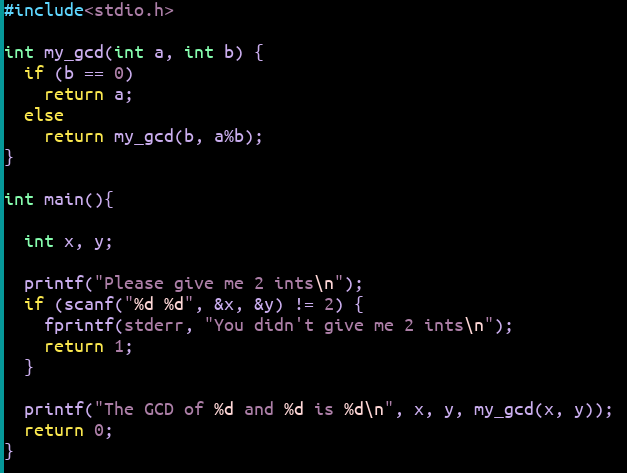
\includegraphics[scale=0.48]{c}\\
\vspace{0.2cm}
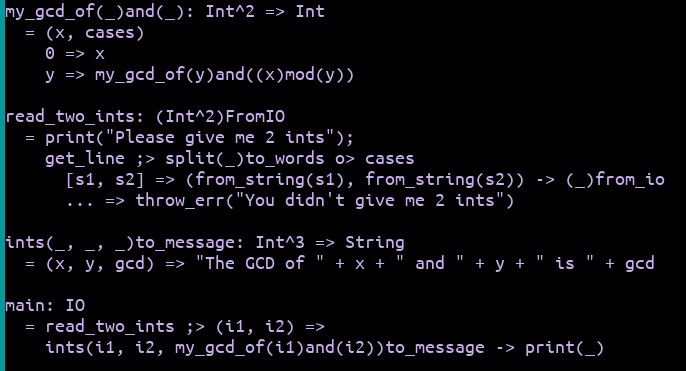
\includegraphics[scale=0.48]{lcases}
\end{center}
\newpage

An important difference between C and lcases is the fact that in lcases the
identifier, the expression of its type and the expression that is assigned to
it are all separated from each other. This is demonstrated by comparing the
"\verb|my_gcd|" function in the C code with the "\verb|my_gcd_of(_)and(_)|" in
lcases. Specifically comparing the line:
\begin{verbatim}
int my_gcd(int a, int b) {
\end{verbatim}
with the line:
\begin{verbatim}
my_gcd_of(_)and(_): Int^2 => Int
\end{verbatim}
we can see that the fact that the function receives two integers and returns an
integer is written in C by giving the type \textbf{\texttt{int}} to each of the
parameters and to the result of the function, while in lcases this is all
written in a single type expression that does not have any identifiers in it.

Also in the same lcases line, we can observe that the identifier has a
parenthesis in the middle which makes it expect the first argument in that
spot. The function is then called recursively with arguments inside the
parentheses in the line:
\begin{verbatim}
y => my_gcd_of(y)and((x)mod(y))
\end{verbatim}
where we can also see that \verb|(_)mod(_)| is defined expecting the first
argument in the beginning. Similarly, \verb|ints(_, _, _)to_message| expects
all three arguments in the same parenthesis in the middle.

Another notable difference is the use of the "cases" keyword in the lines:
\begin{verbatim}
= (x, cases)
  0 => x
  y => my_gcd_of(y)and((x)mod(y))
\end{verbatim}
instead of the "if-then" statement of the lines:
\begin{verbatim}
if (b == 0)
  return a;
else
  return my_gcd(b, a%b);
\end{verbatim}
By using the "cases" keyword in the spot of the second parameter we indicate
that we are going to pattern match on it in the cases. That can be done
for any subset of the parameters (see section \ref{subsubsec:casessyntax}).

Another difference worth mentioning is the use of the plus operator for
string concatenation and also for automatically converting the integers to
strings for them to be concatenated in the line:
\begin{verbatim}
= (x, y, gcd) => "The GCD of " + x + " and " + y + " is " + gcd
\end{verbatim}
as opposed to using "printf" with "\%d" in the line:
\begin{verbatim}
printf("The GCD of %d and %d is %d\n", x, y, my_gcd(x, y));
\end{verbatim}

Finally, another difference is the fact the semicolon is actually an operator
in lcases with environment actions as operands as described in section
\ref{subsec:envacts}.

\newpage
\paragraph{Comparison with \H}
\begin{center}
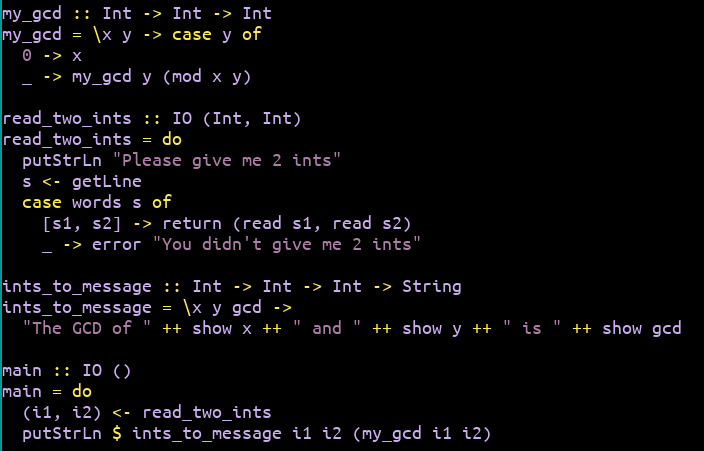
\includegraphics[scale=0.48]{haskell}\\
\vspace{0.2cm}
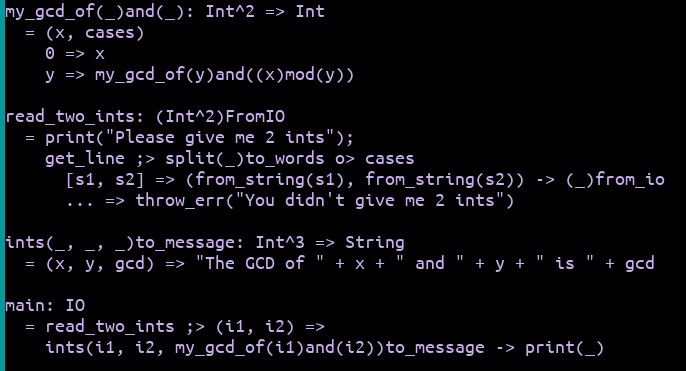
\includegraphics[scale=0.48]{lcases}
\end{center}

An important difference between \H\ and lcases is the fact that in lcases
function application is done with parenthesis instead of spaces which also
gives the opportunity to have arguments inside the function identifier as can
be seen by comparing the line:
\begin{verbatim}
my_gcd :: Int -> Int -> Int
\end{verbatim}
with the line:
\begin{verbatim}
my_gcd_of(_)and(_): Int^2 => Int
\end{verbatim}

In the same lines we can also see that we use one input and one output (as in
\H) but the input is the product type of all the argument types. This might
seem restrictive but in fact it is more general as in lcases it is possible to
provide any subset of the arguments (by putting an underscore in the rest) and
the result is a function that expects the rest of the arguments (unless they
were all provided), see section \ref{subsubsec:parenfuncapp}. In \H\ the
arguments must be provided from left to right and we can omit the n rightmost
arguments for the result to be a function that expects these n arguments.
However, if for example we want to omit the first and provide the second (from
left to right) we must use "flip" first. For more complicated similar stuff
we must define functions similar to "flip" every time by hand.

Also in the same lines we can see the use of the power type \verb|Int^2|
which does not exist in \H.

By comparing the lines:
\begin{verbatim}
my_gcd :: Int -> Int -> Int
my_gcd = \x y -> case y of
\end{verbatim}
with the lines:
\begin{verbatim}
my_gcd_of(_)and(_): Int^2 => Int
  = (x, cases)
\end{verbatim}
we see that in lcases the type annotation and the assignment are grouped into
one to avoid using the identifier twice.

By comparing the lines:
\begin{verbatim}
= (x, cases)
  0 => x
  y => my_gcd_of(y)and((x)mod(y))
\end{verbatim}
with the lines:
\begin{verbatim}
my_gcd = \x y -> case y of
  0 -> x
  _ -> my_gcd y (mod x y)
\end{verbatim}
we see that in lcases we immediately use the "cases" keyword in the parameter
we want to pattern match on without giving it a name. The name is given (if it
is necessary) on the default/last case (if there is one).  The "cases" keyword
can be used on any subset of the parameters to pattern match on all of them at
the same time (see section \ref{subsubsec:casessyntax}).

By comparing the lines:
\begin{verbatim}
= print("Please give me 2 ints");
  get_line ;> split(_)to_words o> cases
\end{verbatim}
with the lines:
\begin{verbatim}
putStrLn "Please give me 2 ints"
s <- getLine
case words s of
\end{verbatim}
we see that in lcases we don't use do notation, instead we use the environment
operators "\verb|;|" and "\verb|;>|" which are the equivalent to the \H\
operators "\verb|>>|" and "\verb|>>=|" respectively (see section
\ref{subsec:envacts}).

Finally, the last difference worth mentioning is the use of the plus operator
for string concatenation and also for automatically converting the integers to
strings for them to be concatenated in the line:
\begin{verbatim}
= (x, y, gcd) => "The GCD of " + x + " and " + y + " is " + gcd
\end{verbatim}
as opposed to using the "\verb|++|" operator and "\verb|show|" in the line:
\begin{verbatim}
"The GCD of " ++ show x ++ " and " ++ show y ++ " is " ++ show gcd
\end{verbatim}

\chapter{Language Description: General}

\section{Program Structure}

An lcases program consists of a set of definitions, type nicknames and
theorems.  Definitions are split into value definitions, type definitions and
type proposition definitions. Theorems are proven type propositions. Functions
as well as "Environment Actions" (see section \ref{subsec:envacts}) are also
considered values. The definition of the "main" value determines the program's
behaviour.

\paragraph{Program example: Euclidean Algorithm}
\begin{verbatim}
gcd_of(_)and(_): Int^2 => Int
  = (x, cases)
    0 => x
    y => gcd_of(y)and((x)mod(y))

read_two_ints: (Int^2)FromIO
  = print("Please give me 2 ints");
    get_line ;> split(_)to_words o> cases
      [x, y] => (from_string(x), from_string(y)) -> (_)from_io
      ... => throw_err("You didn't give me 2 ints")

tuple_type NumsAndGcd
value (x, y, gcd):Int^3

nag(_)to_message: NumsAndGcd => String
  = nag => "The GCD of " + nag.x + " and " + nag.y + " is " + nag.gcd

main: IO
  = read_two_ints ;> (i1, i2) =>
    (i1, i2, gcd_of(i1)and(i2)) -> nag(_)to_message -> print(_)
\end{verbatim}

\paragraph{Program grammar}
\begin{grammar}
<program> ::=
<nl>* <program-part> ( <nl> <nl> <program-part> )* <nl>*

<program-part> ::= ""\\
<value-def> | <grouped-value-defs> | <type-def> | <t-nickname> |
<type-prop-def> | <type-theo>

<nl> :: ( `\ ' | `\\t' )* `\\n'
\end{grammar}

\newpage
\section{Keywords}

The lcases keywords are the following:
\begin{verbatim}
cases all where tuple_type value or_type values
type_proposition needed equivalent type_theorem proof
\end{verbatim}
Each keyword's functionality is described in the respective section shown in
the table below:

\begin{center}
\centering
\begin{tabular}{ |c|c| }
\hline
Keyword & Section
\\
\hline
\hline
\verb|cases| & \ref{subsubsec:casessyntax} "cases" Function Expressions
\\
\hline
\verb|all where| & \ref{subsec:valdefswhere}
Value Definitions and "where" Expressions
\\
\hline

\begin{tabular}{@{}c@{}}
\verb|tuple_type value or_type|
\\
\verb|values type_nickname|
\end{tabular}
&
\ref{subsec:types} Types
\\
\hline
\begin{tabular}{@{}c@{}}
\verb|type_proposition needed|\\
\verb|equivalent type_theorem proof|
\end{tabular}
&
{\ref{subsec:typelogic} Type Logic}
\\
\hline
\end{tabular}

\end{center}
The "\verb|cases|" and "\verb|where|" keywords are also
reserved words. Therefore, even though they can be generated by the
"identifiers" grammar, they cannot be used as identifiers (see "Literals and
Identifiers" section \ref{subsubsec:litsandidents}).

\newpage
\chapter{Language Description: Values}

\section{Basic Expressions}

\subsection{Literals and Identifiers}
\label{subsubsec:litsandidents}

\paragraph{Literals}
\begin{itemize}

\item \textit{Examples}
\begin{verbatim}
1  2  17  42  -100
1.62  2.72  3.14  -1234.567
'a'  'b'  'c'  'x'  'y'  'z'  '.'  ','  '\n'
"Hello World!"  "What's up, doc?"  "Alrighty then!"
\end{verbatim}

\item \textit{Description}

There are literals for the four basic types: \texttt{Int, Real, Char, String}.

\item \textit{Grammar}
\begin{grammar}
<literal> ::= <int-lit> | <real-lit> | <char-lit> | <string-lit>
\end{grammar}

\end{itemize}


\paragraph{Identifiers}
\begin{itemize}

\item \textit{Examples}
\begin{verbatim}
x y z
a1 a2 a3
(_)mod(_)
apply(_)to_all_in(_)
\end{verbatim}

\item \textit{Description}

An identifier is the name of a value or a parameter. It is used in the
definition of a value and in expressions that use that value, or in the
parameters of a function and in the body of that function.
\\\\
An identifier starts with a lower case letter, which can be followed by lower
case letters or underscores and/or ended with a digit. It is also possible to
have underscores in parenthesis before, after or in the middle of an identifier
(see "Parenthesis Function Application" section \ref{subsubsec:parenfuncapp}
for why this can be useful).
\\\\
A simple identifier is an identifier without any underscores in parenthesis.
It used in expressions where underscores in parenthesis don't make sense (e.g.
"Prefix and Postfix Functions" \ref{subsubsec:prefixpostfix}).

\newpage
\item \textit{Grammar}
\begin{grammar}
<identifier> ::=
[ <unders-in-paren> ] <id-start> <id-cont>* [ [0-9] ] [ <unders-in-paren> ]

<simple-id> ::= <id-start> [ [0-9] ]

<id-start> ::= [a-z] [a-z_]*

<id-cont> ::= <unders-in-paren> [a-z_]+

<unders-in-paren> ::= `(_' ( <comma> `_' )* `)'

<comma> ::= `,' [ `\ ' ]
\end{grammar}
Even though the "\verb|cases|" and "\verb|where|" keywords can be generated
by these grammar rules, they cannot be used as identifiers.

\end{itemize}

\newpage
\subsection{Parenthesis, Tuples and Lists}

\paragraph{Parenthesis}

\begin{itemize}

\item \textit{Examples}
\begin{verbatim}
(1 + 2)
(((1 + 2) * 3)^4)
(n => 3*n + 1)
(get_line ;> line => print("Line is: " + line))
\end{verbatim}

\item \textit{Description}

An expression is put in parenthesis to prioritize it or isolate it in a bigger
(operator) expression. The expressions inside parenthesis are operator
or function expressions.
\\\\
Parenthesis expressions cannot extend over multiple lines. For expressions
that extend of over multiple lines new values must be defined.

\item \textit{Grammar}
\begin{grammar}
<paren-expr> ::= `(' [ `\ ' ] <line-op-expr> | <line-func-expr> [ `\ ' ] `)'
\end{grammar}

\end{itemize}

\paragraph{Tuples}

\begin{itemize}

\item \textit{Examples}
\begin{verbatim}
(1, "What's up, doc?")
(2, "Alrighty then!", 3.14)
(x, y, z, w)
(1, my_function, (x, y, z) => sqrt(x^2 + y^2 + z^2))
\end{verbatim}

\item \textit{Description}

Tuples are used to group many values (of possibly different types) into one.
The type of a tuple can be either the product of the types of the fields or a
defined \verb|tuple_type| which is equivalent to the aforementioned product
type (see "Tuple Types" in section \ref{subsubsec:tdefs} for details). For
example, the type of the second tuple above could be:
\begin{verbatim}
Int x String x Real
\end{verbatim}
or:
\begin{verbatim}
MyType
\end{verbatim}
assuming "\verb|MyType|" has been defined in a similar way to the following:
\begin{verbatim}
tuple_type MyType
value
  (my_int, my_string, my_real) : Int x String x Real
\end{verbatim}

\newpage
\item \textit{Big Tuples}
\\\\
\textbf{Example}
\begin{verbatim}
my_big_tuple
  : String x Int x Real x String x String x (String x Real x Real)
  = ( "Hey, I'm the first field and I'm also a relatively big string."
    , 42, 3.14, "Hey, I'm the first small string", "Hey, I'm the second small string"
    , ("Hey, I'm a string inside the nested tuple", 2.72, 1.62)
    )
\end{verbatim}

\textbf{Description}

It is possible to stretch a (big) tuple expression over multiple lines (only)
in a separate value definition (see "Value Definitions" section
\ref{subsubsec:valdefs}).  In that case:
\begin{itemize}
\item
The character '\verb|(|' is after the "\verb|=| " part of the value definition
and the first field must be in the same line.

\item
The tuple can split in a new line only at a '\verb|,|' character. Every such
line must be indented so that the '\verb|,|' is in same column where the
'\verb|(|' character was in the first line.

\item
The tuple must be ended by a line that only contains the '\verb|)|' character
and is also indented so that the '\verb|)|' is in same column where the
'\verb|(|' character was in the first line.

\item
The precise indentation rules are described in the section
"Indentation System" \ref{subsubsec:indsys}.
\end{itemize}

\item \textit{Tuples with empty fields}
\\\\
\textbf{Examples}
\begin{verbatim}
(42, _)
(_, 3.14, _)
(_, _, "Hello from 3rd field")
\end{verbatim}

\textbf{Description}\\\\
It is possible to leave some fields empty in a tuple by having an underscore in
their position. This creates a function that expects the empty fields
and returns the whole tuple. This is best demonstrated by the types of the
examples above:
\begin{verbatim}
(42, _) : T1 => Int x T1
(_, 3.14, _) : T1 x T2 => T1 x Real x T2
(_, _, "Hello from 3rd field") : T1 x T2 => T1 x T2 x String
\end{verbatim}
An example in a bigger expression is the following:
\begin{verbatim}
questions : ListOf(String)s
  = ["the Ultimate Question of Life", "the Universe", "Everything"]

answers_to : ListOf(String)s
  = apply("The answer to " + _)to_all_in(questions)
\end{verbatim}

\newpage
\begin{verbatim}
>> apply((42, _))to_all_in(answers_to)
  : ListOf(Int x String)s
  ==> [ (42, "The answer to the Ultimate Question of Life")
      , (42, "The answer to the Universe")
      , (42, "The answer to Everything")
      ]
\end{verbatim}

\item \textit{Grammar}
\begin{grammar}
<tuple> ::=
`(' [ `\ ' ] <line-expr-or-under> <comma> <line-expr-or-unders> [ `\ ' ] `)'

<line-expr-or-unders> ::=
<line-expr-or-under> ( <comma> <line-expr-or-under> )*

<line-expr-or-under> ::= <line-expr> | `_'

<line-expr> ::= <basic-or-app-expr> | <line-op-expr> | <line-func-expr>

<basic-or-app-expr> ::= <basic-expr> | <pre-func-app> | <post-func-app>

<basic-expr> ::=
<literal> | <paren-func-app-or-id> | <special-id> | <tuple> | <list>
\\

<big-tuple> ::= ""\\
`(' [ `\ ' ] <line-expr-or-under> [ <nl> <indent> ]
<comma> <line-expr-or-unders> \\
( <nl> <indent> <comma> <line-expr-or-unders> )* \\
<nl> <indent> `)'
\end{grammar}

\end{itemize}

\paragraph{Lists}

\begin{itemize}

\item \textit{Examples}
\begin{verbatim}
[1, 2, 17, 42, -100]
[1.62, 2.72, 3.14, -1234.567]
["Hello World!", "What's up, doc?", "Alrighty then!"]
[x => x + 1, x => x + 2, x => x + 3]
[x, y, z, w]
\end{verbatim}

\item \textit{Description}

Lists are used to group many values of the same type into one.  The type of the
list is \verb|ListOf(T1)s| where \verb|T1| is the type of every value inside.
Therefore, the types of the first four examples are:
\begin{verbatim}
ListOf(Int)s
ListOf(Real)s
ListOf(String)s
(@A)And(Int)Add_To(@B) --> ListOf(@A => @B)s
\end{verbatim}
And the last list is only legal if x, y, z and w all have the same type.
Assuming they do and it's the type T, the type of the list is:
\begin{verbatim}
ListOf(T)s
\end{verbatim}

\newpage
\item \textit{Big Lists}
  \\\\
  \textbf{Example}

  \begin{verbatim}
my_big_list: ListOf(Int => IO)s
  = [ x => print("I'm the first function and x + 1 is: " + (x + 1))
    , x => print("I'm the second function and x + 2 is: " + (x + 2))
    , x => print("I'm the third function and x + 3 is: " + (x + 3))
    ]
  \end{verbatim}

  \textbf{Description}

  It is possible to stretch a (big) list expression over multiple lines (only)
  in a separate value definition (see "Value Definitions" section
  \ref{subsubsec:valdefs}).  In that case:
  \begin{itemize}
  \item
  The character '\verb|[|' is after the "= " part of the value definition
  and the first element must be in the same line.

  \item
  The list can split in a new line only at a '\verb|,|' character. Every such
  line must be indented so that the '\verb|,|' is in same column where the
  '\verb|[|' character was in the first line.

  \item
  The list must be ended by a line that only contains the '\verb|]|' character
  and is also indented so that the '\verb|]|' is in same column where the
  '\verb|[|' character was in the first line.

  \item
  The precise indentation rules are described in the section
  "Indentation System" \ref{subsubsec:indsys}.
  \end{itemize}

\item \textit{Grammar}
\begin{grammar}
<list> ::= `[' [ `\ ' ] [ <line-expr-or-unders> ] [ `\ ' ] `]'

<big-list> ::= ""\\
`[' [ `\ ' ] <line-expr-or-unders> \\
( <nl> <indent> <comma> <line-expr-or-unders> )* \\
<nl> <indent> `]'
\end{grammar}

\end{itemize}

\newpage
\subsection{Parenthesis Function Application}
\label{subsubsec:parenfuncapp}

\begin{itemize}
\item \textit{Examples}

\begin{verbatim}
f(x)
f(x, y, z)
(x)to_string
apply(f)to_all_in(l)
\end{verbatim}

\item \textit{Description}

Function application in lcases can be done in many different ways. In this
section, we discuss the ways function application can be done with parenthesis.
\\\\
In the first two examples, the usual mathematical function application is used
which is also used in most programming languages and should be familiar to the
reader, i.e. function application is done with the arguments of the function in
parenthesis separated by commas and \textbf{appended} to the function
identifier.
\\\\
This idea can be extended by allowing the arguments to be \textbf{prepended} or
to be \textbf{inside} to the function identifier (examples 3 and 4). This is
only valid if the function has been \textbf{defined with these parentheses in
the identifier}. For example, the definition for
"\verb|apply(_)to_all_in(_)|"
starts like so:
\begin{verbatim}
apply(_)to_all_in(_) : (T1 => T2) x ListOf(T1)s => ListOf(T2)s
  = <...definition>
\end{verbatim}
The identifier is "\verb|apply(_)to_all_in(_)|" with the parentheses
\textbf{included}.  This is very useful for defining functions where the
argument in the middle or before makes the function application look and sound
more like natural language.
\\\\
It is possible to have many parentheses in a single function application (last
example). The arguments are always inserted to the function from \textbf{left
to right}.  Therefore, when multiple parentheses are present the arguments of
the leftmost parentheses are inserted first then the next ones to the right and
so on.

\newpage
\item \textit{Empty arguments in Parenthesis Function Application}
\\\\
It is possible to provide a function with a subset its arguments by putting an
underscore to all the missing arguments. The resulting expression is a function
that expects the missing arguments to return the final result. Let's see
this in action:
\begin{verbatim}
f(_, _, _) : Char x Int x Real => String
c, i, r : Char, Int, Real

f(c, i, r) : String

f(_, i, r) : Char => String
f(c, _, r) : Int => String
f(c, i, _) : Real => String

f(c, _, _) : Int x Real => String
f(_, i, _) : Char x Real => String
f(_, _, r) : Char x Int => String
\end{verbatim}

\item \textit{Grammar}
\begin{grammar}
<paren-func-app-or-id> ::= ""\\""
[ <arguments> ] <id-start> ( <arguments> [a-z_]+ )* [ [0-9] ]
[ <arguments> ]

<arguments> ::= `(' [ `\ ' ] <line-expr-or-unders> [ `\ ' ] `)'

\end{grammar}

\end{itemize}

\newpage

\subsection{Prefix and Postfix Functions}
\label{subsubsec:prefixpostfix}

\paragraph{Prefix Functions}

\begin{itemize}

\item \textit{Examples}
\begin{verbatim}
the_value:1
error:e
result:r
apply(the_value:_)to_all_in(_)
\end{verbatim}

\item \textit{Description}

Prefix functions are automatically generated from \verb|or_type| definitions
(see "Or Types" in section \ref{subsubsec:tdefs}). They are functions that
convert a value of a particular type to a value that is a case of an
\verb|or_type| and has values of the first type inside. For example in the
first example above we have:
\begin{verbatim}
1 : Int
the_value:1 : Possibly(Int)
\end{verbatim}
Where the function \verb|the_value:_| is automatically generated from the
definition of the \verb|Possibly(_)| type:
\begin{verbatim}
or_type Possibly(T1)
values the_value:T1 | no_value
\end{verbatim}
And it has the type \verb|T1 => Possibly(T1)|.
\\\\
These functions are called prefix functions because they are prepended to their
argument. However, they can also be used as arguments to other functions with
an underscore in their argument.  This is illustrated in the last example,
where the function \verb|the_value:_| is an argument of the function
\verb|apply(_)to_all_in(_)|.

\item \textit{Grammar}
\begin{grammar}
<pre-func> ::= <simple-id> `:'

<pre-func-app> ::= <pre-func> <operand>
\end{grammar}

\end{itemize}

\newpage
\paragraph{Postfix Functions}

\begin{itemize}

\item \textit{Examples}
\begin{verbatim}
name.first_name
list.head
date.year
tuple.1st
apply(_.1st)to_all_in(_)
\end{verbatim}

\item \textit{Description}

Postfix functions are automatically generated from \verb|tuple_type|
definitions (see "Tuple Types" in section \ref{subsubsec:tdefs}). They are
functions that take a \verb|tuple_type| value and return a particular field
(i.e. projection functions). For example in the first example above we have:
\begin{verbatim}
name : Name
name.first_name : String
\end{verbatim}
Where the function \verb|_.first_name| is automatically generated from the
definition of the \verb|Name| type:
\begin{verbatim}
tuple_type Name
value (first_name, last_name) : String^2
\end{verbatim}
And it has the type \verb|Name => String|.
\\\\
There are also the following special projection functions that work on all
tuples that are of a product type:
"\verb|_.1st|", "\verb|_.2nd|", "\verb|_.3rd|", "\verb|_.4th|", "\verb|_.5th|"
.
For the 4th example above, assuming:
\begin{verbatim}
tuple : Int x String
\end{verbatim}
We have:
\begin{verbatim}
tuple.1st : Int
\end{verbatim}
The general types of these functions are:
\begin{verbatim}
_.1st : (@A)Is(@B)s_1st --> @B => @A
_.2nd : (@A)Is(@B)s_2nd --> @B => @A
...
\end{verbatim}
These functions are called postfix functions because they are appended to their
argument. However, they can also be used as arguments to other functions with
an underscore in their argument. This is illustrated in the last example, where
the function "\verb|_.1st|" is an argument of the function
"\verb|apply(_)to_all_in(_)|".
\\\\
There is a special postfix function called "\verb|_.change|" which is described
in the following paragraph.

\newpage
\item \textit{Grammar}
\begin{grammar}
<post-func> ::= `.' ( <simple-id> | <special-id> )

<special-id> ::= `1st' | `2nd' | `3rd' | `4th' | `5th'

<post-func-app> ::= ""\\
( <basic-expr> | <paren-expr> | `_' )
( <dot-change> | <post-func>+ [ <dot-change> ] )
\end{grammar}

\end{itemize}

\paragraph{The ".change" Function}

\begin{itemize}

\item \textit{Examples}

\begin{verbatim}
state.change{counter = counter + 1}
tuple.change{1st = 42, 3rd = 17}
point.change{x = 1.62, y = 2.72, z = 3.14}
apply(_.change{1st = 1st + 1})to_all_in(_)
x.change{1st = _, 3rd = _}
\end{verbatim}

\item \textit{Description}
\\\\
The "\verb|_.change|" function is a special postfix function that works an all
tuples. It returns a new tuple that is the same as the input tuple except for
some changed fields. Which fields change and to what new value is specified
inside curly brackets after the "\verb|.change|". The following special
identifiers can be used for referring to the fields of product type tuples:
"\verb|1st|", "\verb|2nd|", "\verb|3rd|", "\verb|4th|", "\verb|5th|"
(2nd, 4th and 5th example). If the tuple is of a tuple type, the identifiers of
the fields specified in the type definition are used (1st and 3rd example).
Therefore, we are assuming the following (or similar) if the examples are to
type check:

\begin{verbatim}
tuple_type MyStateType
value (..., counter, ...) : ... x Int x ...

state : MyStateType


tuple : Int x SomeType x Int (x ...)


tuple_type Point
value (x, y, z) : Real^3

point : Point


apply(_.change{1st = 1st + 1})to_all_in(_)
  : (@A)And(Int)AddTo(@A), (@A)Is(@B)s_1st --> ListOf(@B)s => ListOf(@B)s


x : Int x Real x String
x.change{1st = _, 3rd = _} : Int x String => Int x Real x String
\end{verbatim}

\newpage
The changes of the fields have the following structure:
"\verb|field = <expression of new value>|"
and they are separated by commas. The input tuple's fields (i.e. the
"old" values) can be used inside the expression of a new value and they are
referred to by the field identifier (1st and 4th example). Underscores can be
used as the expressions of some new values which makes the whole expression
a function that expects those new values as arguments (last example).
\item \textit{Grammar}

\begin{grammar}
<dot-change> ::=
`.change{' [ `\ ' ] <field-change> ( <comma> <field-change> )* [ `\ ' ] `}'

<field-change> ::= ( <simple-id> | <special-id> ) <equals> <line-expr-or-under>

<equals> ::= [ `\ ' ] `=' [ `\ ' ]
\end{grammar}

\end{itemize}

\section{Operators}

\subsection{Function Application and Function Composition Operators}

\paragraph{Function Application Operators}

\begin{center}
\begin{tabular}{ |c|c|c| }
\hline
Operator & Type
\\
\hline
\hline
\verb|->| & \verb| T1 x (T1 => T2) => T2|
\\
\hline
\verb|<-| & \verb| (T1 => T2) x T1 => T2|
\\
\hline
\end{tabular}
\end{center}
The function application operators "\verb|->|" and "\verb|<-|" are a
different way to apply functions to arguments than the usual parenthesis
function application.  They are meant to look like arrows that point from the
argument to the function.  These operators are very useful for chaining many
function applications without the clutter of having to open and close
parentheses for each one of the functions.  For example, assuming we have the
following functions with the behaviour suggested by their names and types:
\begin{verbatim}
apply(_)to_all_in(_) : (T1 => T2) x ListOf(T1)s => ListOf(T2)s
str_len(_) : String => Int
filter(_)with(_) : ListOf(T1)s x (T1 => Bool) => ListOf(T1)s
(_)is_odd : Int => Bool
sum_ints(_) : ListOf(Int)s => Int
\end{verbatim}
And a list of strings:
\begin{verbatim}
strings : ListOf(String)s
\end{verbatim}
Here is a simple way to get the total number of characters in all the strings
that have odd length:
\begin{verbatim}
chars_in_odd_length_strings : Int
  = apply(str_len(_))to_all_in(strings) -> filter(_)with((_)is_odd) -> sum_ints(_)
\end{verbatim}
This can be done equivalently using the other operator:
\begin{verbatim}
chars_in_odd_length_strings : Int
  = sum_ints(_) <- filter(_)with((_)is_odd) <- apply(str_len(_))to_all_in(strings)

\end{verbatim}

\newpage

\paragraph{Function Composition Operators}
\begin{center}
\begin{tabular}{ |c|c|c| }
\hline
Operator & Type
\\
\hline
\hline
\verb|o>| & \verb|(T1 => T2) x (T2 => T3) => (T1 => T3)|
\\
\hline
\verb|<o| & \verb|(T2 => T3) x (T1 => T2) => (T1 => T3)|
\\
\hline
\end{tabular}
\end{center}
The function composition operators "\verb|o>|" and "\verb|<o|" are used to
compose functions, each one in the corresponding direction. The use of the
letter '\verb|o|' is meant to be similar to the mathematical function
composition symbol '\(\circ\)' and the symbols '\verb|>|', '\verb|<|' are used
so that the operator points from the function which is applied first to the
function which is applied second.  A neat example using function composition is
the following. Assuming we have the following functions with the behaviour
suggested by their names and types:
\begin{verbatim}
split(_)to_words : String => ListOf(String)s
apply(_)to_all_in(_) : (T1 => T2) x ListOf(T1)s => ListOf(T2)s
reverse_str(_) : String => String
merge_words(_) : ListOf(String)s => String
\end{verbatim}
We can reverse the all the words in a string like so:
\begin{verbatim}
reverse_words_in(_) : String => String
  = split(_)to_words o> apply(reverse_str(_))to_all_in(_) o> merge_words(_)
\end{verbatim}
This can be done equivalently using the other operator:
\begin{verbatim}
reverse_words_in(_) : String => String
  = merge_words(_) <o apply(reverse_str(_))to_all_in(_) <o split(_)to_words
\end{verbatim}

\newpage

\subsection{Arithmetic, Comparison and Boolean Operators}

\paragraph{Arithmetic Operators}
\begin{center}
\begin{tabular}{ |c|c|c| }
\hline
Operator & Type
\\
\hline
\hline
\verb|^| & \verb|(@A)To_The(@B)Is(@C) --> @A x @B => @C|
\\
\hline
\verb|*| & \verb|(@A)And(@B)Multiply_To(@C) --> @A x @B => @C|
\\
\hline
\verb|/| & \verb|(@A)Divided_By(@B)Is(@C) --> @A x @B => @C|
\\
\hline
\verb|+| & \verb|(@A)And(@B)Add_To(@C) --> @A x @B => @C|
\\
\hline
\verb|-| & \verb|(@A)Minus(@B)Is(@C) --> @A x @B => @C|
\\
\hline
\end{tabular}
\end{center}
The usual arithmetic operators work as they are expected, similarly to
mathematics and other programming languages for the usual types. However, they
are generalized. The examples below show their generality:
\begin{verbatim}
>> 1 + 1
  : Int
  ==> 2
>> 1 + 3.14
  : Real
  ==> 4.14
>> 'a' + 'b'
  : String
  ==> "ab"
>> 'w' + "ord"
  : String
  ==> "word"
>> "Hello " + "World!"
  : String
  ==> "Hello World!"
>> 5 * 'a'
  : String
  ==> "aaaaa"
>> 5 * "hi"
  : String
  ==> "hihihihihi"
>> "1,2,3" - ','
  : String
  ==> "123"
\end{verbatim}
Let's analyze further the example of addition. The type can be read as such:
the '\verb|+|' operator has the type \\ \verb|@A x @B => @C|, provided that the
type proposition \verb|(@A)And(@B)Add_To(@C)| holds. This proposition being
true, means that addition has been defined for these three types (see section
"Type Logic" \ref{subsec:typelogic} for more on type propositions). Therefore,
by the examples above we can deduce that the following propositions
are true (in the order of the examples):
\begin{verbatim}
(Int)And(Int)Add_To(Int)
(Int)And(Real)Add_To(Real)
(Char)And(Char)Add_To(String)
(Char)And(String)Add_To(String)
(Int)And(Char)Multiply_To(String)
(Int)And(String)Multiply_To(String)
(String)Minus(Char)Is(String)
\end{verbatim}
This allows us to use the familiar arithmetic operators in types that are not
necessarily numbers but it is somewhat intuitively obvious what they should do
in those other types. Furthermore, their behaviour can be defined by the user
for new user defined types!

\paragraph{Comparison, Boolean and Bitwise Operators}

\begin{center}
\begin{tabular}{ |c|c|c| }
\hline
Operator & Type
\\
\hline
\hline
\verb|==| & \verb|(@A)And(@B)Can_Be_Equal --> @A x @B => Bool|
\\
\hline
\verb|!=| & \verb|(@A)And(@B)Can_Be_Unequal --> @A x @B => Bool|
\\
\hline
\verb|>| & \verb|(@A)Can_Be_Greater_Than(@B) --> @A x @B => Bool|
\\
\hline
\verb|<| & \verb|(@A)Can_Be_Less_Than(@B) --> @A x @B => Bool|
\\
\hline
\verb|>=| & \verb|(@A)Can_Be_Gr_Or_Eq_To(@B) --> @A x @B => Bool|
\\
\hline
\verb|<=| & \verb|(@A)Can_Be_Le_Or_Eq_To(@B) --> @A x @B => Bool|
\\
\hline
\verb|&| & \verb|(@A)Has_And --> @A^2 => @A|
\\
\hline
\texttt{|} & \verb|(@A)Has_Or --> @A^2 => @A|
\\
\hline
\end{tabular}
\end{center}
Comparison operators are also generalized. The main reason for the
generalization is to be able to compare numbers of different types. Consider
the following example:

\begin{verbatim}
>> 1
  : Int
  ==> 1
>> 1.1
  : Real
  ==> 1.1
>> 1.1 == 1
  : Bool
  ==> false
>> 1.0 == 1
  : Bool
  ==> true
\end{verbatim}
In order for the example to work we need to be able to compare integers and
reals.  Similarly, all the comparison operators need to be able to work on
arguments of different types.
\\\\
Boolean "and" and bitwise "and" are combined into one general "and" operator
(\verb|&|). The same applies to the "or" operator (\texttt{|}).

\newpage

\subsection{Environment Action Operators}
\label{subsec:envacts}

\begin{center}
\begin{tabular}{ |c|c|c| }
\hline
Operator & Type
\\
\hline
\hline
\verb|;>| & \verb|(@E(_))Has_Use --> @E(T1) x (T1 => @E(T2)) => @E(T2)|
\\
\hline
\verb|;| & \verb|(@E(_))Has_Then --> @E(T1) x @E(T2) => @E(T2)|
\\
\hline
\end{tabular}
\end{center}

\paragraph{Simple Example Program}
\begin{verbatim}
main: (EmptyVal)FromIO
  = print_string("I'll repeat the line") ; get_line ;> print_string(_)
\end{verbatim}
The example above demonstrates the use of the environment action operators with
the \verb|(_)FromIO| environment type, which is how IO is done in lcases. Some
light can be shed on how this is done, if we take a look at the types (as
always!):
\begin{verbatim}
print_string(_): String => (EmptyVal)FromIO
print_string("I'll repeat the line"): (EmptyVal)FromIO
get_line: (String)FromIO


\end{verbatim}
For the "then" operator we have:
\verb|; : (@E(_))Has_Then --> @E(T1) x @E(T2) => @E(T2)|
\\\\
In the following expression:
\verb|print_string("I'll repeat the line") ; get_line|
\\
the "then" operator has type:
\verb|(EmptyVal)FromIO x (String)FromIO => SomeType|
\\\\
The only way to match the types is:
\\
\verb|  @E(_) = (_)FromIO, T1 = EmptyVal, T2 = String and SomeType = (String)FromIO|
\\
and it type checks because: \verb|((_)FromIO)Has_Then|
\\\\
For the whole expression we have:
\begin{verbatim}
print_string("I'll repeat the line") ; get_line
  : (String)FromIO


\end{verbatim}
For the "use" operator we have:
\verb|;> : (@E(_))Has_Use --> @E(T1) x (T1 => @E(T2)) => @E(T2)|
\\\\
In the following expression:
\verb|print_string("I'll repeat the line") ; get_line ;> print_string(_)|
\\
the "use" operator has type:
\verb|(String)FromIO x (String => (EmptyVal)FromIO) => SomeType|
\\\\
The only way to match the types is:
\\
\verb|  @E(_) = FromIO, T1 = String, T2 = EmptyVal and SomeType = (EmptyVal)FromIO|
\\
and it type checks because: \verb|((_)FromIO)Has_Use|
\\\\
For the whole expression we have:
\begin{verbatim}
print_string("I'll repeat the line") ; get_line ;> print_string(_)
  : (EmptyVal)FromIO
\end{verbatim}

\newpage
\paragraph{Another Example Program}
\begin{verbatim}
main: (EmptyVal)FromIO
  = print_string("Hello! What's your name?") ; get_line ;> name =>
    print_string("And how old are you?") ; get_line ;> age =>
    print_string("Oh! You don't look " + age + " " + name + "!")

print_string(_): String => (EmptyVal)FromIO

print_string("Hello! What's your name?") : (EmptyVal)FromIO

print_string("Hello! What's your name?"); get_line
  : (String)FromIO

print_string("And how old are you?"); get_line
  : (String)FromIO

print_string("Oh! You don't look " + age + " " + name + "!")
  : (EmptyVal)FromIO

age => print_string("Oh! You don't look " + age + " " + name + "!")
  : String => (EmptyVal)FromIO

print_string("And how old are you?") ; get_line ;> age =>
print_string("Oh! You don't look " + age + " " + name + "!")
  : (EmptyVal)FromIO

name =>
print_string("And how old are you?") ; get_line ;> age =>
print_string("Oh! You don't look " + age + " " + name + "!")
  : String => (EmptyVal)FromIO

print_string("Hello! What's your name?") ; get_line ;> name =>
print_string("And how old are you?") ; get_line ;> age =>
print_string("Oh! You don't look " + age + " " + name + "!")
  : (EmptyVal)FromIO
\end{verbatim}

\newpage
\paragraph{Description}\pend
The environment action operators are used to combine values that do environment
actions into values that do more complicated environment actions. Environment
types are type functions that take a type argument and produce a type
(just like \verb|ListOf(_)s|). These types have the "then" operator
(\verb|;|) and the "use" operator (\verb|;>|) defined for them.  A value of the
type \verb|@E(T1)| where \verb|(@E)Has_Then| does an environment action of type
\verb|@E(_)| that produces a value of type \verb|T1| which can then be combined
with another one with the "then" operator. Similarly, with the "use" operator
the produced value of an action can be used by a function that returns another
action.
\\\\
The effect of the "\verb|;|" operator described in words is the following:
given a value of type \verb|@E(T1)| and a value of type \verb|@E(T2)|
(which are environment actions that produce values of type \verb|T1| and
\verb|T2| respectively), create a new value the does both actions (provided
the first did not result in an error).  The overall effect is a value which is
an environment action of type \verb|@E(_)| (the combination of the "smaller"
actions) which produces a value of type \verb|T2| (the one produced by the
second action) and therefore it is of type \verb|@E(T2)|.
\\\\
Note that the value of type \verb|T1| produced by the first action is not
used anywhere. This happens mostly when \verb|T1 = EmptyVal| and it is
because values of type \verb|@E(EmptyVal)| are used for their environment
action only \\(e.g. \verb|print_string(...): (EmptyVal)FromIO|).
\\\\
How the two environment actions of the \verb|@E(T1)| and \verb|@E(T2)|
values are combined to produce the new environment action is specific to the
environment action type \verb|@E(_)|.
\\\\
The effect of the "\verb|;>|" operator described in words is the following:
given a value of type \verb|@E(T1)| (which is an environment action of type
\verb|@E(_)| that produces a value of type \verb|T1|) and a value of type
\verb|T1 => @E(T2)| (which is a function that takes a value of type
\verb|T1| and returns an environment action of type \verb|@E(_)| that produces
a value of type \verb|T2|), combine those two values by creating a value that
does the following:
\begin{itemize}
\item
Performs the first action that produces a value of type \verb|T1|

\item
Takes the value of type \verb|T1| produced (provided there was no error) and
passes it to the function of type \verb|T1 => @E(T2)| that then returns an
action

\item
Performs the resulting action
\end{itemize}
The overall effect is an environment action  of type \verb|@E(_)| that produces
a value is of type \verb|T2| and therefore the new value is of type
\verb|@E(T2)|.

\newpage

\subsection{Operator Expressions}

\begin{itemize}
\item \textit{Examples}
\begin{verbatim}
1 + 2
1 + x * 3^y
"Hello " + "World!"
x -> f -> g
f o> g o> h
x == y
x >= y - z & x < 2 * y
get_line ; get_line ;> line => print("Second line: " + line)
2 * _
_ - 1
"Hello " + "it's me, " + _
"Hi, I am " + _ + " and I am " + _ + " years old"
\end{verbatim}

\item \textit{Description}

Operator expressions are expressions that are comprised of operators and
operands. Operators act like two-argument-functions that are placed in between
their arguments (operands).  Therefore, they have function types and they act
as it is described in their respective sections above this one.
\\\\
An operator expression might have multiple operators. The order of operations
is explained in the next section ("Complete Operator Table, Precedence and
Associativity") in Table \ref{table:precassoc}.
\\\\
Just like functions, the operands of an operator, must have types that match
the types expected by the operator.
\\\\
It is possible for the second operand of an operator to be a function
expression.  This is mostly useful with the "\verb|;>|" operator (see
previous section: "Environment Operators").
\\\\
It is possible to use an underscore as an operand. An operator expression with
underscore operands becomes a function that expects those operands as
arguments.  This is best demonstrated by the types of the last four examples:

\begin{verbatim}
2 * _ : Int => Int
_ - 1 : Int => Int
"Hello " + "it's me, " + _ : String => String
"Hi, I am " + _ + " and I am " + _ + " years old" : String^2 => String
\end{verbatim}
Note: These are not the most general types for these examples but they are
compatible.

\newpage

\item \textit{Big Operator Expressions}\\\\
\textbf{Example}

\begin{verbatim}
"Hello, I'm a big string that's going to contain multiple values from " +
"inside the imaginary program that I'm a part of. Here they are:\n" +
"value1 = " + value1 + ", value2 = " + value2 + ", value3 = " + value3 +
", value4 = " + value4 + ", value5 = " + value5
\end{verbatim}

\textbf{Description}

It is possible to stretch a (big) operator expression over multiple lines.
In that case:
\begin{itemize}
\item
The operator expression must split in a new line after an operator (not an
operand).

\item
Every line after the first must be indented so that in begins at the column
where the first line of the operator expression begun.

\item
The precise indentation rules are described in the section
"Indentation System" \ref{subsubsec:indsys}.
\end{itemize}

\item \textit{Grammar}
\begin{grammar}
<op-expr> ::= <line-op-expr> | <big-op-expr>
\\

<op-expr-start> ::= ( <operand> <op> )+

<line-op-expr> ::= <op-expr-start> ( <operand> | <line-func-expr> )
\\

<big-op-expr> ::=
<big-op-expr-op-split> | <big-op-expr-func-split>
\\

<big-op-expr-op-split> ::=
<op-split-line>+ [ <op-expr-start> ] ( <operand> | <func-expr> )

<op-split-line> ::=
( <op-expr-start> ( <nl> | <oper-fco> ) | <oper-fco> ) <indent>

<oper-fco> ::= <operand> `\ ' <func-comp-op> `\\n'
\\

<big-op-expr-func-split> ::=
<op-expr-start> ( <big-func-expr> | <cases-func-expr> )
\\

<operand> ::= <basic-or-app-expr> | <paren-expr> | `_'
\\

<op> ::= `\ ' <func-comp-op> `\ ' | [ `\ ' ] <optional-spaces-op> [ `\ ' ]

<func-comp-op> ::= `o>' | `<o'

<optional-spaces-op> ::= ""\\
`->' | `<-' | `^' | `*' | `/' | `+' | `-' | `==' | `!=' | `>' | `<' | `>=' |
`<=' | `\&' | `|' | `;>' | `;'
\end{grammar}
\end{itemize}

\newpage
\subsection{Complete Operator Table, Precedence and Associativity}

\begin{table}[h]

\caption{
The complete operator table of lcases operators along with their types and
their short descriptions.
}

\begin{center}
\begin{tabular}{ |c|c|c| }
\hline
Op & Type & Description
\\
\hline
\hline
\verb|->| & \verb|T1 x (T1 => T2) => T2| &
\begin{tabular}{@{}c@{}}
Right Function
\\
Application
\end{tabular}
\\
\hline
\verb|<-| & \verb|(T1 => T2) x T1 => T2| &
\begin{tabular}{@{}c@{}}
Left Function
\\
Application
\end{tabular}
\\
\hline
\verb|o>| & \verb|(T1 => T2) x (T2 => T3) => (T1 => T3)| &
\begin{tabular}{@{}c@{}}
Right Function
\\
Composition
\end{tabular}
\\
\hline
\verb|<o| & \verb|(T2 => T3) x (T1 => T2) => (T1 => T3)| &
\begin{tabular}{@{}c@{}}
Left Function
\\
Composition
\end{tabular}
\\
\hline
\verb|^| & \verb|(@A)To_The(@B)Is(@C) --> @A x @B => @C| &
General Exponentiation
\\
\hline
\verb|*| & \verb|(@A)And(@B)Multiply_To(@C) --> @A x @B => @C| &
General Multiplication
\\
\hline
\verb|/| & \verb|(@A)Divided_By(@B)Is(@C) --> @A x @B => @C| &
General Division
\\
\hline
\verb|+| & \verb|(@A)And(@B)Add_To(@C) --> @A x @B => @C| &
General Addition
\\
\hline
\verb|-| & \verb|(@A)Minus(@B)Is(@C) --> @A x @B => @C| &
General Subtraction
\\
\hline
\verb|==| & \verb|(@A)And(@B)Can_Be_Equal --> @A x @B => Bool| &
General Equality
\\
\hline
\verb|!=| & \verb|(@A)And(@B)Can_Be_Unequal --> @A x @B => Bool| &
General Inequality
\\
\hline
\verb|>| & \verb|(@A)Can_Be_Greater_Than(@B) --> @A x @B => Bool| &
General Greater Than
\\
\hline
\verb|<| & \verb|(@A)Can_Be_Less_Than(@B) --> @A x @B => Bool| &
General Less Than
\\
\hline
\verb|>=| & \verb|(@A)Can_Be_Gr_Or_Eq_To(@B) --> @A x @B => Bool| &
\begin{tabular}{@{}c@{}}
General Greater Than
\\
or Equal To
\end{tabular}
\\
\hline
\verb|<=| & \verb|(@A)Can_Be_Le_Or_Eq_To(@B) --> @A x @B => Bool| &
\begin{tabular}{@{}c@{}}
General Less Than
\\
or Equal To
\end{tabular}
\\
\hline
\verb|&| & \verb|(@A)Has_And --> @A^2 => @A| & General And
\\
\hline
\texttt{|} & \verb|(@A)Has_Or --> @A^2 => @A| & General Or
\\
\hline
\verb|;>| & \verb|(@E(_))Has_Use --> @E(T1) x (T1 => @E(T2)) => @E(T2)| &
\begin{tabular}{@{}c@{}}
"Use"
\\
Environment Action
\end{tabular}
\\
\hline
\verb|;| & \verb|(@E(_))Has_Then --> @E(T1) x @E(T2) => @E(T2)| &
\begin{tabular}{@{}c@{}}
"Then"
\\
Environment Action
\end{tabular}
\\
\hline
\end{tabular}
\end{center}

\label{table:allops}

\end{table}
\newpage\noindent
The order of operations is done from highest to lowest precedence. In the same
level of precedence the order is done from left to right if the associativity
is "Left" and from right to left if the associativity is "Right". For the
operators that have associativity "None" it is not allowed to place them in the
same operator expression. The precedence and associativity of the operators
is shown in the table below.

\begin{table}[h]

\caption{ The table of precedence and associativity of the lcases operators.  }

\begin{center}
\begin{tabular}{ |c|c|c| }
\hline
Operator & Precedence & Associativity
\\
\hline
\hline
\verb|->| & 10 (highest) & Left
\\
\hline
\verb|<-| & 9 & Right
\\
\hline
\verb|o> <o| & 8 & Left
\\
\hline
\verb|^| & 7 & Right
\\
\hline
\verb|* /| & 6 & Left
\\
\hline
\verb|+ -| & 5 & Left
\\
\hline
\verb|== != > < >= <=| & 4 & None
\\
\hline
\verb|&| & 3 & Left
\\
\hline
\texttt{|} & 2 & Left
\\
\hline
\verb|;> ;| & 1 & Left
\\
\hline
\end{tabular}
\end{center}

\label{table:precassoc}

\end{table}

\newpage
\section{Function Expressions}
\label{subsec:funcexprs}

Function expressions are divided into \textbf{regular function expressions} and
\textbf{"cases" function expressions} which are described in the following
sections.
\begin{grammar}
<func-expr> ::= <line-func-expr> | <big-func-expr> | <cases-func-expr>
\end{grammar}

\subsection{Regular Function Expressions}

\begin{itemize}
\item \textit{Examples}

\begin{verbatim}
a => 17 * a + 42
(a, b) => a + 2*b
(x, y, z) => sqrt(x^2 + y^2 + z^2)
* => 42
(x, *, z) => x + z
((x1, y1), (x2, y2)) => (x1 + x2, y1 + y2)
\end{verbatim}

\item \textit{Description}

Regular function expressions are used to define functions or be part of bigger
expressions as anonymous functions. They are comprised by their parameters and
their body.
\\\\
Parameters have identifiers. There is either only one parameter, in which case
there is no parenthesis, or there are many, in which case they are in
parentheses, separated by commas. If a parameter is not needed it can be left
empty by having an asterisk instead of an identifier (4th and 5th example).
If a parameter is a tuple itself it can be matched further by using parentheses
and giving identifiers to its fields (6th example).
\\\\
The parameters and the body are separated by the function arrow
("\verb|=>|"). The body is a basic expression, an operator expression or
a function expression in parenthesis.

\item \textit{Big Function Expressions}\\\\
\textbf{Example}

\begin{verbatim}
(value1, value2, value3, value4, value5, value6, value7) =>
print("value1 = " + value1 + ", value2 = " + value2 + ", value3 = " + value3) ;
print("value4 = " + value4 + ", value5 = " + value5 + ", value6 = " + value6) ;
print("value7 = " + value7)
\end{verbatim}

\textbf{Description}

It is possible to stretch a (big) function expression over multiple lines.
In that case:
\begin{itemize}
\item
The function expression must split in a new line after the function arrow
("\verb|=>|").

\item
Every line after the first must be indented so that in begins at the column
where the first character of the parameters was in the first line.

\item
The precise indentation rules are described in the section
"Indentation System" \ref{subsubsec:indsys}.
\end{itemize}

\newpage
\item \textit{Grammar}
\begin{grammar}
<line-func-expr> ::= <parameters> [ `\ ' ] `=>' <line-func-body>

<big-func-expr> ::= <parameters> [ `\ ' ] `=>' <big-func-body>

<parameters> ::= ""\\
<identifier> | `*' |
`(' [ `\ ' ] <parameters> ( <comma> <parameters> )+ [ `\ ' ] `)'

<line-func-body> ::= ""\\""
[ `\ ' ]
(
<basic-or-app-expr> | <line-op-expr> |
`(' [ `\ ' ] <line-func-expr> [ `\ ' ] `)'
)

<big-func-body> ::= ""\\
<nl> <indent>
(
<basic-or-app-expr> | <op-expr> | `(' [ `\ ' ] <line-func-expr> [ `\ ' ] `)'
)
\end{grammar}
\end{itemize}

\newpage
\subsection{"cases" Function Expressions}
\label{subsubsec:casessyntax}

\begin{itemize}
\item \textit{Examples}

\begin{verbatim}
print_sentimental_bool(_): Bool => IO
  = cases
    true => print("It's true!! :)")
    false => print("It's false... :(")

or_type TrafficLight
values green | amber | red

(_)is_not_red: TrafficLight => Bool
  = cases
    green => true
    amber => true
    red => false

(_)is_seventeen_or_forty_two: Int => Bool
  = cases
    17 => true
    42 => true
    ... => false

traffic_lights_match(_, _): TrafficLight^2 => Bool
  = (cases, cases)
    (green, green) => true
    (amber, amber) => true
    (red, red) => true
    ... => false

gcd_of(_)and(_): Int^2 => Int
  = (x, cases)
    0 => x
    y => gcd_of(y)and((x)mod(y))

apply(_)to_all_in(_): (T1 => T2) x ListOf(T1)s => ListOf(T2)s
  = (f(_), cases)
    [] => []
    [head, tail = ...] => f(head) + apply(f(_))to_all_in(tail)

(_)is_sorted: (@A)Has_Less_Than_Or_Equal --> ListOf(@A)s => Bool
  = cases
    [x1, x2, xs = ...] => (x1 < x2) & (x2 + xs)is_sorted
    ... => true
\end{verbatim}

\newpage

\item \textit{Description}

"\verb|cases|" is a keyword that works as a special parameter.  Instead of
giving the name "\verb|cases|" to that parameter, it is used to pattern match
on the possible values of that parameter and return a different result for each
particular case.
\\\\
The last case can be "\verb|... => (body of default case)|" to capture all
remaining cases while dismissing the value (e.g.
"\verb|is_seventeen_or_forty_two|" example), or it can be \\
"\verb|some_id => (body of default case)|" to capture all remaining
cases while being able to use the value with the name "\verb|some_id|"
(e.g.  "\verb|y|" in "\verb|gcd|" example).
\\\\
It is possible to use "\verb|cases|" in multiple parameters to match on all of
them combined. By doing that, each case represents a particular combination of
values for the "\verb|cases|" parameters involved\\(e.g.
\verb|traffic_lights_match| example).
\\\\
It is also possible to use a "\verb|where|" expression below a particular case.
The "\verb|where|" expression must be indented two spaces more than than the
line where that particular case begins.
\\\\
It is also possible to use the following syntax to match on as many elements of
a list as needed and optionally give a name to the rest of the list:
\begin{verbatim}
# no name for the rest of the list
[x1, ...] => <case body>
[x1, x2, ...] => <case body>
[x1, x2, x3, ...] => <case body>

# name for the rest of the list
[x1, xs = ...] => <case body>
[x1, x2, xs = ...] => <case body>
[x1, x2, x3, xs = ...] => <case body>
\end{verbatim}

\newpage
\item \textit{Grammar}
\begin{grammar}
<cases-func-expr> ::= <cases-params> <case>+ [ <end-case> ]

<cases-params> ::=
""\\
<identifier> | `cases' | `*' | ""\\
`(' [ `\ ' ] <cases-params> ( <comma> <cases-params> )+ [ `\ ' ] `)'
\\

<case> ::=  <nl> <indent> <outer-matching> [ `\ ' ] `=>' <case-body>

<end-case> ::=
<nl> <indent> ( `...' | <identifier> ) [ `\ ' ] `=>' <case-body>
\\

<outer-matching> ::= <simple-id> | <matching>

<matching> ::=
<literal> | <pre-func> <inner-matching> | <tuple-matching> | <list-matching>

<inner-matching> ::= `*' | <identifier> | <matching>

<tuple-matching> ::=
`(' [ `\ ' ] <inner-matching> ( <comma> <inner-matching> )+ [ `\ ' ] `)'

<list-matching> ::= ""\\
`[' [ `\ ' ]
[ <inner-matching> ( <comma> <inner-matching> )* [ <rest-list-matching> ] ]
""\\""
[ `\ ' ] `]'

<rest-list-matching> ::= <comma> [ <simple-id> <equals> ] `...'
\\

<case-body> ::= <line-func-body> | <big-func-body> [ <where-expr> ]
\end{grammar}

\end{itemize}

\newpage

\section{Value Definitions and "where" Expressions}
\label{subsec:valdefswhere}

\subsection{Value Definitions}
\label{subsubsec:valdefs}

\begin{itemize}

\item \textit{Examples}

\begin{verbatim}
foo: Int
  = 42

f(_, _, _): Int^3 => Int
  = (a, b, c) => a + b * c

val1, val2, val3: Int, Bool, Char
  = 42, true, 'a'

int1, int2, int3: all Int
  = 1, 2, 3
\end{verbatim}

\item \textit{Description}

Value definitions are the main building block of lcases programs. To define a
new value you give it a name, a type and an expression. The name is an
identifier which is followed by the "has type" symbol ('\verb|:|') and the
expression of the type of the value. The line below is indented two spaces and
begins with the equal sign and continues with the expression of the value
(which extends to as many lines as needed).
\\\\
A value definition begins either in the first column, where it can be "seen" by
all other value definitions, or it is inside a "\verb|where|" expression (see
section below), where it can be "seen" by the expression above the
"\verb|where|" and all the other definitions in the same "\verb|where|"
expression.
\\\\
A value definition can be followed by a "\verb|where|" expression where
intermediate values used in the value expression are defined. In that case, the
"\verb|where|" expression must be indented two spaces more than the "\verb|=|"
line of the value definition.
\\\\
It is possible to group value definitions together by separating the names, the
types and the expressions with commas. This is very useful for not cluttering
the program with many definitions for values with small expressions (e.g.
constants).  When grouping definitions together it is also possible to use the
keyword "\verb|all|" to give the same type to all the values.

\item \textit{Grammar}
\begin{grammar}
<value-def> ::= ""\\
<indent> <identifier>
( [ `\ ' ] `:' [ `\ ' ] | <nl> <indent> `:\ ' ) <type>  \\
<nl> <indent> `=\ ' <value-expr> [ <where-expr> ]

<value-expr> ::=
<basic-or-app-expr> | <op-expr> | <func-expr> | <big-tuple> | <big-list>
\\

<grouped-value-defs> ::= ""\\
<indent> <identifier> ( <comma> <identifier> )+ \\
( [ `\ ' ] `:' [ `\ ' ] | <nl> <indent> `:\ ' )
( <type> ( <comma> <type> )+ | `all\ ' <type> ) \\
<nl> <indent> `=\ ' <line-exprs> ( <nl> <indent> <comma> <line-exprs> )*

<line-exprs> ::= <line-expr> ( <comma> <line-expr> )*
\end{grammar}

\end{itemize}

\newpage

\subsection{"where" Expressions}
\label{subsubsec:whereexprs}

\begin{itemize}

\item \textit{Examples}
\begin{verbatim}
sort(_): ListOf(Int)s => ListOf(Int)s
  = cases
    [] => []
    [head, tail = ...] =>
      sort(less_l) + head + sort(greater_l)
      where
      less_l, greater_l: all ListOf(Int)s
        = filter(tail)with(_ < head), filter(tail)with(_ >= head)

sum_nodes(_): TreeOf(Int)s => Int
  = tree =>
    tree.root + apply(sum_nodes(_))to_all_in(tree.subtrees) -> sum_list(_)
    where
    sum_list(_) : ListOf(Int)s => Int
      = cases
        [] => 0
        [head, tail = ...] => head + sum_list(tail)

big_string : String
  = s1 + s2 + s3 + s4
    where
    s1, s2, s3, s4 : all String
      = "Hello, my name is Struggling Programmer."
      , " I have tried way too many times to fit a big chunk of text"
      , " inside my program, without it hitting the half-screen mark!"
      , " I am so glad I finally discovered lcases!"
\end{verbatim}

\item \textit{Description}

"\verb|where|" expressions allow the programmer to use values inside an
expression and define them below it. They are very useful for reusing or
abbreviating expressions that are specific to a particular definition or case.
\\\\
A "\verb|where|" expression begins by a line that only has the word
"\verb|where|" in it. It is indented as described in the "Value Definitions"
(\ref{subsubsec:valdefs}) or "'cases' Function Expressions"
(\ref{subsubsec:casessyntax}) sections.  The definitions are placed below the
"\verb|where|" line and must have the same indentation.

\item \textit{Grammar}
\begin{grammar}
<where-expr> ::= ""\\
<nl> <indent> `where'
<nl> <value-def-or-defs> ( <nl> <nl> <value-def-or-defs> )*

<value-def-or-defs> ::= <value-def> | <grouped-value-defs>
\end{grammar}

\end{itemize}

\newpage

\chapter{Language Description: Types and Type Logic}

\section{Types}
\label{subsec:types}

The constructs regarding types are \textbf{type expressions}, \textbf{type
definitions} and \textbf{type nicknames} and they are described in the
following sections.

\subsection{Type Expressions}

Type expressions are divided into the following categories:
\begin{itemize}
\item Type Identifiers
\item Type Variables
\item Type Application Types
\item Product Types
\item Function Types
\item Conditional Types
\end{itemize}
which are described in the following paragraphs.
\\\\
The grammar of a type expression is:
\begin{grammar}
<type> ::= [ <condition> ]  <simple-type>

<simple-type> ::=
<param-t-var> | <type-app-id-or-ahtv> | <power-type> | <prod-type> |
<func-type>
\end{grammar}

\paragraph{Type Identifiers}

\begin{itemize}
\item \textit{Examples}
\begin{verbatim}
Int     Real     Char     String     SelfReferencingType
\end{verbatim}

\item \textit{Description}

A type identifier is either the name of a basic type (Int, Real, Char, String)
or the name of some defined type that has no type parameters. It begins with a
capital letter and is followed by capital or lowercase letters.

\item \textit{Grammar}
\begin{grammar}
<type-id> ::= [A-Z] [A-Za-z]*
\end{grammar}
\end{itemize}

\paragraph{Type Variables}\pend
Type Variables are placeholders inside bigger type expressions that can be
substituted with various types. This makes the bigger type expression an
expression of a \textbf{polymorphic} type. The types of polymorphism that exist
in lcases are \textbf{parametric polymorphism} and \textbf{ad hoc
polymorphism}. Type variables for each of the two types have different syntax
and they are described in the following paragraphs.

\subparagraph{Parametric Type Variables}

\begin{itemize}
\item \textit{Examples}
\begin{verbatim}
T1     T2     T3
\end{verbatim}

\item
\textit{Examples of parametric type variables inside bigger type expressions}
\begin{verbatim}
T1 => T1
(T1 => T2) x (T2 => T3) => (T1 => T3)
(T1^2 => T1) x T1 x ListOf(T1)s => T1
\end{verbatim}

\item \textit{Description}

Parametric type variables can be substituted with any type and the program will
type check.  The simplest example of a polymorphic type with a parametric type
variable is the type of the identity function where we have:
\begin{verbatim}
id(_): T1 => T1
  = x => x

id(1): Int
  where T1 is substituted by Int and id gets the type Int => Int

id("Hello"): String
  where T1 is substituted by String and id gets the type String => String
\end{verbatim}

A parametric type variable is written with capital "T" followed by a digit.

\item \textit{Grammar}
\begin{grammar}
<param-t-var> ::= `T' [0-9] \\
\end{grammar}
\end{itemize}

\subparagraph{Ad Hoc Type Variables}

\begin{itemize}
\item \textit{Examples}
\begin{verbatim}
@A @B @C @T
\end{verbatim}

\item \textit{Examples of ad hoc type variables inside bigger type expressions}
\begin{verbatim}
(@T)Has_Str_Rep --> @T => String
(@A)Is(@B)s_First --> @B => @A
(@A)And(@B)Can_Be_Equal --> @A x @B => Bool
(@A)And(@B)Add_To(@C) --> @A x @B => @C
\end{verbatim}

\item \textit{Description}

Ad hoc type variables are type variables that can be substituted only by types
that satisfy a condition. This condition comes in the form of a type
proposition (see Type Logic section \ref{subsec:typelogic}). Therefore, any ad
hoc type variable must also appear in the condition as shown in the examples.
\\\\
An ad hoc type variable is written with an '@' followed by any capital letter.

\item \textit{Grammar}
\begin{grammar}
<ad-hoc-t-var> ::= `@' [A-Z]
\end{grammar}
\end{itemize}

\paragraph{Type Application Types}

\begin{itemize}
\item \textit{Examples}
\begin{verbatim}
Possibly(Int)
ListOf(Real)s
TreeOf(String)s
Result(Int)OrError(String)
ListOf(Int => Int)s
ListOf(T1)s
\end{verbatim}

\item \textit{Description}

Type application types are types that are produced by passing type arguments to
a type function generated by a \verb|tuple_type| definition, an \verb|or_type|
definition or a \verb|type_nickname|. For example, given the definition of
\verb|Possibly(T1)|:
\begin{verbatim}
or_type Possibly(T1)
values the_value:T1 | no_value
\end{verbatim}
We have that \verb|Possibly(_)| is a type function that receives one type
parameter and returns a resulting type. For example \verb|Possibly(Int)| is
the result of passing the type argument \verb|Int| to \verb|Possibly(_)|.
\\\\
Type application types have the same form as the name in the \verb|tuple_type|
definition, \verb|or_type| definition or \verb|type_nickname|, with the
difference that type parameters are substituted by the expressions of the type
arguments.

\item \textit{Grammar}
\begin{grammar}
<type-app-id-or-ahtv> ::=
[ <types-in-paren> ] <taioa-middle> [ <types-in-paren> ]

<taioa-middle> ::=
<type-id> ( <types-in-paren> [A-Za-z]+ )* | <ad-hoc-t-var>

<types-in-paren> ::=
`(' [ `\ ' ] <simple-type> ( <comma> <simple-type> )* [ `\ ' ] `)'
\end{grammar}
\end{itemize}

\newpage

\paragraph{Product Types}

\begin{itemize}
\item \textit{Examples}
\begin{verbatim}
Int x Real x String
ListOf(Int)s x Int x ListOf(String)s
(Int => Int) x (Int x Real) x (Real => String)
Int^2 x Int^2
Real^3 x Real^3
\end{verbatim}

\item \textit{Description}

Product types are the types of tuples. They are comprised of the expressions of
the types of the fields separated by the string " \verb|x| " (space '\verb|x|'
space) to resemble the cartesian product. If any of the fields is of a product
or a function type then the corresponding type expression must be inside
parentheses. A product type where all the fields are of the same type can be
abbreviated with a power type expression which is comprised of the type, the
power symbol '\verb|^|' and the number of times the type is repeated.

\item \textit{Grammar}
\begin{grammar}
<prod-type> ::= <field-type> ( `\ x\ ' <field-type> )+

<field-type> ::= <power-base-type> | <power-type>

<power-base-type> ::= ""\\
<param-t-var> | <type-app-id-or-ahtv> |
`(' [ `\ ' ] ( <prod-type> | <func-type> ) [ `\ ' ] `)'

<power-type> ::= <power-base-type> `^' <int-greater-than-one>
\end{grammar}
\end{itemize}

\paragraph{Function Types}

\begin{itemize}
\item \textit{Examples}
\begin{verbatim}
String => String
Real => Int
T1 => T1
Int^2 => Int
Real^3 => Real
(T1 => T2) x (T2 => T3) => (T1 => T3)
(Int => Int) => (Int => Int)
\end{verbatim}

\item \textit{Description}

A function type expression is comprised of the input type expression and the
output type expression separated by the function arrow ("\verb|=>|"). The
input and output type expressions are type expressions which are put in
parentheses only if they are function type expressions.

\item \textit{Grammar}
\begin{grammar}
<func-type> ::= <in-or-out-type> `\ =>\ ' <in-or-out-type>

<in-or-out-type> ::=
""\\
<param-t-var> | <type-app-id-or-ahtv> | <power-type> | <prod-type> | ""\\
`(' [ `\ ' ] <func-type>  [ `\ ' ] `)'
\end{grammar}
\end{itemize}

\newpage

\paragraph{Conditional Types}

\begin{itemize}
\item \textit{Examples}
\begin{verbatim}
(@A)And(@B)Can_Be_Equal --> @A x @B => Bool
(@A)And(@B)Add_To(@C) --> @A x @B => @C
(@A)Is(@B)s_First --> @B => @A
(@T)Has_Str_Rep --> @T => String
(@E(_))Has_Use --> @E(T1) x (T1 => @E(T2)) => @E(T2)
\end{verbatim}

\item \textit{Description}

Conditional types are the types of values that are polymorphic not because of
their structure but because they have been defined (separately) for many
different combinations of types (i.e. they are ad hoc polymorphic). They are
comprised of a condition and a "simple" type (i.e. a type without a condition)
which are separated by the condition arrow (" \verb|-->| "). The condition is
a type proposition which refers to type variables inside the "simple" type and
it must hold whenever the polymorphic value of that type is used. For example:
\begin{verbatim}
(_)first: (@A)Is(@B)s_First --> @B => @A
\end{verbatim}
can be used as follows:
\begin{verbatim}
pair, triple, list
  : Int x String, Real x Char x Int, ListOf(String)s
  = (42, "The answer to everything"), (3.14, 'a', 1), ["Hi!", "Hello", Heeey"]

>> (pair)first
  : Int
  ==> 42
>> (triple)first
  : Real
  ==> 3.14
>> (list)first
  : String
  ==> "Hi!"
\end{verbatim}
and that is because the following propositions hold:
\begin{verbatim}
(Int)Is(Int x String)s_First
(Real)Is(Real x Char x Int)s_First
(String)Is(ListOf(String)s)s_First
\end{verbatim}
which it turn means that the function "\verb|(_)first|" has been defined for these
combinations of types. For more on how conditions, propositions and ad hoc
polymorphism works, see the "Type Logic" section (\ref{subsec:typelogic}).

\item \textit{Grammar}
\begin{grammar}
<condition> ::= <prop-name> `\ -->\ '
\end{grammar}

\end{itemize}

\newpage

\subsection{Type Definitions}
\label{subsubsec:tdefs}

Type definitions are divided into \verb|tuple_type| definitions and
\verb|or_type| definitions which are described in the following paragraphs.
\\\\
The grammar of a type definition is:
\begin{grammar}
<type-def> ::= <tuple-type-def> | <or-type-def>
\end{grammar}

\paragraph{Tuple Types}

\begin{itemize}
\item \textit{Definition Examples}

\begin{verbatim}
tuple_type Name
value (first_name, last_name) : String^2

tuple_type Date
value (day, month, year) : Int^3

tuple_type MathematicianInfo
value (name, nationality, date_of_birth) : Name x String x Date

tuple_type TreeOf(T1)s
value (root, subtrees) : T1 x ListOf(TreeOf(T1)s)s

tuple_type Indexed(T1)
value (index, val) : Int x T1
\end{verbatim}

\item \textit{Usage Examples}

\begin{verbatim}
euler_info: MathematicianInfo
  = (("Leonhard", "Euler"), "Swiss", (15, 4, 1707))

name(_)to_string: Name => String
  = n => "\nFirst Name: " + n.first_name + "\nLast Name: " + n.last_name

print_name_and_nat(_): MathematicianInfo => IO
  = ci => print(name(ci.name)to_string + "\nNationality: " + ci.nationality)

sum_nodes(_): TreeOf(Int)s => Int
  = tree => tree.root + apply(sum_nodes(_))to_all_in(tree.subtrees) -> sum_list(_)
\end{verbatim}

\item \textit{Description}

A tuple type is equivalent to a product type with a new name  and names for the
fields for convenience. A tuple type generates postfix functions for all of
the fields by using a '.' before the name of the field. For example the
"\verb|MathematicianInfo|" type above generates the following functions:
\begin{verbatim}
_.name : MathematicianInfo => Name
_.nationality : MathematicianInfo => String
_.date_of_birth : MathematicianInfo => Date
\end{verbatim}

\newpage

\item \textit{Grammar}

\begin{grammar}
<tuple-type-def> ::= ""\\
`tuple_type\ ' <type-name> <nl> \\
`value' ( `\ ' | <nl> `\ \ ' )
<id-tuple> [ `\ ' ] `:' [ `\ ' ] ( <prod-type> | <power-type> )

<type-name> ::= ""\\""
[ <param-vars-in-paren> ] <type-id> ( <param-vars-in-paren> [A-Za-z]+ )* ""\\""
[ <param-vars-in-paren> ]

<param-vars-in-paren> ::=
`(' [ `\ ' ] <param-t-var> ( <comma> <param-t-var> )* [ `\ ' ] `)'

<id-tuple> ::= `(' [ `\ ' ] <simple-id> ( <comma> <simple-id> )+ [ `\ ' ] `)'
\end{grammar}

\end{itemize}

\paragraph{Or Types}

\begin{itemize}
\item \textit{Definition Examples}

\begin{verbatim}
or_type Bool
values true | false

or_type TrafficLight
values green | amber | red

or_type Possibly(T1)
values the_value:T1 | no_value

or_type Result(T1)OrError(T2)
values result:T1 | error:T2
\end{verbatim}

\item \textit{Usage Examples}

\begin{verbatim}
traffic_lights_match(_, _): TrafficLight^2 => Bool
  = (cases, cases)
    (green, green) => true
    (amber, amber) => true
    (red, red) => true
    ... => false

err_if(_)is_no_value : Possibly(T1) => Result(T1)OrError(String)
  = cases
    no_value => error:"There is no value!"
    the_value:val => result:val

print_err(_)or_res(_): (@A)Has_Str_Rep --> Result(@A)OrError(String) => IO
  = cases
    result:r => print("All good! The result is: " + (r)to_string)
    error:e => print("Error occured: " + e)
\end{verbatim}

\newpage
\item \textit{Description}

The values of an \verb|or_type| are split into cases. Some cases have other
values inside.  The cases which have other values inside are followed by a
colon and the type of the internal value. Similar syntax can be used for
matching that particular case in a function using the "cases" syntax.  An
\verb|or_type| definition automatically creates prefix functions for each case
with an internal value (which are simply conversions from the type of the
internal value to the \verb|or_type|).  For example, for the case
"\verb|the_value|" of a "\verb|Possibly(T1)|" the function "\verb|the_value:_|"
is automatically created from the definition for which we can say:
\begin{verbatim}
the_value:_ : T1 => Possibly(T1)
\end{verbatim}
These functions can be used like any other function as arguments to other
functions.  For example:
\begin{verbatim}
(_)to_possiblies : ListOf(T1)s => ListOf(Possibly(T1))s
  = apply(the_value:_)to_all_in(_)
\end{verbatim}

\item \textit{Grammar}

\begin{grammar}
<or-type-def> ::= ""\\
`or_type\ ' <type-name> <nl> \\
`values' ( `\ ' | <nl> `\ \ ' ) \\
<simple-id> [ `:' <simple-type> ]
( [ `\ ' ] `|' [ `\ ' ] <simple-id> [ `:' <simple-type> ] )*
\end{grammar}

\end{itemize}

\subsection{Type Nicknames}

\begin{itemize}

\item \textit{Examples}

\begin{verbatim}
type_nickname Ints = ListOf(Int)s
type_nickname IntStringPairs = ListOf(Int x String)s
type_nickname IO = (EmptyVal)FromIO
type_nickname Res(T1)OrErr = Result(T1)OrError(String)
\end{verbatim}

\item \textit{Description} \\\\
Type nicknames are used to abbreviate or give a more descriptive name to a
type.  They start with the keyword "\verb|type_nickname|", followed by the
nickname, then an equal sign and the type to be nicknamed.
Parametric type variables can be used in the nickname.

\item \textit{Grammar}

\begin{grammar}
<t-nickname> ::=
`type_nickname\ ' <type-name> <equals> <simple-type>
\end{grammar}

\end{itemize}

\newpage
\section{Type Logic}
\label{subsec:typelogic}

Type logic is the mechanism for ad hoc polymorphism in lcases. The central
notion of \textbf{type logic} is the \textbf{type proposition}. A type
proposition is a proposition that has types as parameters and is true or false
for particular type arguments.
\\\\
Type propositions can either be defined or proven (for certain type arguments).
Therefore, the following constructs exist and accomplish the aforementioned
respectively: \textbf{type proposition definitions} and \textbf{type theorems}.
These constructs are described in detail in the following sections. From this
point onwards the "type" part will be omitted, i.e. propositions are always
type propositions and theorems are always type theorems.

\subsection{Proposition Definitions}

Proposition definitions are split into definitions of \textbf{atomic
propositions} and definitions of \textbf{renaming propositions} which are
described in the following paragraphs.

\paragraph{Atomic Propositions}

\begin{itemize}
\item \textit{Examples}
\begin{verbatim}
type_proposition (@A)Is(@B)s_First
needed (_)first: @B => @A

type_proposition (@T)Has_Str_Rep
needed (_)to_string: @T => String

type_proposition (@T)Has_A_Wrapper
needed wrap(_): T1 => @T(T1)

type_proposition (@T)Has_Internal_App
needed apply(_)inside(_) : (T1 => T2) x @T(T1) => @T(T2)
\end{verbatim}
The examples above define the following (ad hoc) polymorphic functions which
have the respective (conditional) types:
\begin{verbatim}
(_)first: (@A)Is(@B)s_First --> @B => @A

(_)to_string: (@T)Has_Str_Rep --> @T => String

wrap(_): (@T)Has_A_Wrapper --> T1 => @T(T1)

apply(_)inside(_): (@T)Has_Internal_App --> (T1 => T2) x @T(T1) => @T(T2)
\end{verbatim}

\newpage

\item \textit{Description}

An atomic proposition definition defines simultaneously the \textbf{atomic
proposition} itself and a \textbf{polymorphic value} (usually, but not
necessarily, a function), by defining the form of the type of the value given
the type parameters of the proposition. The proposition is true or false when
the type parameters are substituted by specific type arguments depending on
whether the implementation of the value has been defined for these type
arguments. The aforementioned truth value determines whether the value is used
correctly inside the program and therefore whether the program will typecheck.
In order to add more types for which the function works, i.e.  define the
function for these types, i.e. make the proposition true for these types, one
must prove a theorem. The specifics of theorems are described in the next
section. For now, we'll show the example for everything mentioned in this
paragraph for the proposition "\verb|(@A)Is(@B)s_First|":

\begin{itemize}
\item Proposition Definition:

\begin{verbatim}
type_proposition (@A)Is(@B)s_First
needed (_)first: @B => @A
\end{verbatim}

\item Function defined and its type:

\begin{verbatim}
(_)first: (@A)Is(@B)s_First --> @B => @A
\end{verbatim}

\item Theorems for specific types:

\begin{verbatim}
type_theorem (T1)Is(T1 x T2)s_First
proof (_)first = _.1st

type_theorem (T1)Is(ListOf(T1)s)s_First
proof
  (_)first =
    cases
      [] => throw_err("Tried to take the first element of an empty list")
      [head, ...] => head
\end{verbatim}

\item Usage of the function
\begin{verbatim}
pair, list
  : Int x String, ListOf(String)s
  = (42, "The answer to everything"), ["Hi!", "Hello", Heeey"]

>> (pair)first
  : Int
  ==> 42
>> (list)first
  : String
  ==> "Hi!"
\end{verbatim}
\end{itemize}

An atomic proposition definition begins with the keyword
"\verb|type_proposition|" followed by the name of the proposition (including
the type parameters) in the first line. The second line begins with the keyword
"\verb|needed|" which is followed by the identifier and the
type expression of the value separated by the "has type" symbol ('\verb|:|').

\end{itemize}

\newpage

\paragraph{Renaming Propositions}

\begin{itemize}
\item \textit{Examples}
\begin{verbatim}
type_proposition (@T)Has_Equality
equivalent (@T)And(@T)Can_Be_Equal

type_proposition (@A)And(@B)Are_Comparable
equivalent
  (@A)Can_Be_Less_Than(@B), (@A)And(@B)Can_Be_Equal, (@A)Can_Be_Greater_Than(@B)

type_proposition (@T)Has_Comparison
equivalent (@T)And(@T)Are_Comparable
\end{verbatim}

\item \textit{Description}

A renaming proposition definition is used to abbreviate one or the conjunction
of many propositions into a new proposition.
\\\\
A renaming proposition definition begins with the keyword
"\verb|type_proposition|" followed by the name of the proposition (including
the type parameters) in the first line. The second line begins with the keyword
"\verb|equivalent|" followed by either one proposition or (if it is a
conjunction) many propositions separated by commas (where the commas
mean "and").

\end{itemize}

\paragraph{Grammar for Proposition Definitions}

\begin{grammar}
<type-prop-def> ::= <atom-prop-def> | <renaming-prop-def>
\\

<atom-prop-def> ::= ""\\
<prop-name-line> <nl> `needed' ( `\ ' | <nl> `\ \ ' )
<identifier> [ `\ ' ] `:' [ `\ ' ] <simple-type>

<renaming-prop-def> ::= ""\\
<prop-name-line> <nl>
`equivalent' ( `\ ' | <nl> `\ \ ' ) <prop-name> ( <comma> <prop-name> )*

<prop-name-line> ::= `type_proposition\ ' <prop-name>

<prop-name> ::=  ""\\""
[A-Z] ( <name-part> <types-in-paren> )+ [ <name-part> ]
\alt " "( <types-in-paren> <name-part> )+ [ <types-in-paren> ]

<name-part> ::= ( [A-Za-z] | `_'[A-Z] )+
\end{grammar}

\newpage

\subsection{Theorems}
\label{subsubsec:ttheo}

Theorems are split into theorems of \textbf{atomic propositions} and
theorems of \textbf{implication propositions} which are described in the
following paragraphs.

\paragraph{Atomic Propositions}

\begin{itemize}
\item \textit{Examples}

\begin{verbatim}
type_theorem (Possibly(_))Has_A_Wrapper
proof wrap(_) = the_value:_

type_theorem (ListOf(_)s)Has_A_Wrapper
proof wrap(_) = [_]

type_theorem (Possibly(_))Has_Internal_App
proof
  apply(_)inside(_) =
    (f(_), cases)
      no_value => no_value
      the_value:x => the_value:f(x)

type_theorem (ListOf(_)s)Has_Internal_App
proof apply(_)inside(_) = apply(_)to_all_in(_)
\end{verbatim}

\item \textit{Usage}

\begin{verbatim}
a, b : all Possibly(Int)
  = wrapper(1), no_value

l1, l2, l3 : all ListOf(Int)s
  = wrapper(1), empty_l, [1, 2, 3]

>> a
  : Possibly(Int)
  ==> the_value:1
>> b
  : Possibly(Int)
  ==> no_value
>> l1
  : ListOf(Int)s
  ==> [1]
>> l2
  : ListOf(Int)s
  ==> []
\end{verbatim}
\newpage
\begin{verbatim}
>> apply(_ + 1)inside(a)
  : Possibly(Int)
  ==> the_value:2
>> apply(_ + 1)inside(b)
  : Possibly(Int)
  ==> no_value
>> apply(_ + 1)inside(l1)
  : ListOf(Int)s
  ==> [2]
>> apply(_ + 1)inside(l2)
  : ListOf(Int)s
  ==> []
>> apply(_ + 1)inside(l3)
  : ListOf(Int)s
  ==> [2, 3, 4]
\end{verbatim}

\item \textit{Description}

A theorem of an atomic proposition proves the proposition for
specific type arguments, by implementing the value associated to the
proposition for these type arguments. Therefore, the value associated with the
proposition can be used with all the combinations of type arguments for which
the proposition is true, i.e. the combinations of type arguments for which
the value has been implemented.
\\\\
A proof of a theorem of an atomic proposition is correct when the
implementation of the value associated with the proposition follows the form of
the type given to the value by the definition of the proposition, i.e. the only
difference between the type of the value in the theorem and the type of the
value in the definition is that the type parameters of the proposition are
substituted by the type arguments of the theorem.
\\\\
A theorem of an atomic proposition begins with the keyword
"\verb|type_theorem|" followed by the name of the proposition with the type
parameters substituted by the specific types for which the proposition will be
proven. The second line is the keyword "\verb|proof|". The third line is
indented once and it is the line in which the proof begins. The proof begins
with the identifier of the value associated with the proposition and is
followed by an equal sign and the value expression which implements the value.

\end{itemize}

\newpage

\paragraph{Implication Propositions}

\begin{itemize}
\item \textit{Examples}

\begin{verbatim}
type_theorem (@A)And(@B)Can_Be_Equal --> (@A)And(@B)Can_Be_Unequal
proof a \= b = not(a == b)

type_theorem (@A)Can_Be_Greater_Than(@B) --> (@A)Can_Be_Le_Or_Eq_To(@B)
proof a <= b = not(a > b)

type_proposition (@A)And(@B)Have_Eq_And_Gr
equivalent (@A)And(@B)Can_Be_Equal, (@A)Can_Be_Greater_Than(@B)

type_theorem (@A)And(@B)Have_Eq_And_Gr --> (@A)Can_Be_Gr_Or_Eq_To(@B)
proof a >= b = a == b | a > b
\end{verbatim}

\item \textit{Description}

A theorem of an implication proposition is similar to a theorem of an atomic
proposition but it also uses other ad hoc polymorphic values in the
implementation. Therefore, the implementation does not prove the proposition
associated to the value it implements unless the polymorphic values used in the
implementation are already defined in their own theorems. In other words it
proves the following: "if these ad hoc polymorphic values are defined then we
can also define this other one". This can be translated into the following
implication proposition: "if the propositions associated to the values we are
using are true then the proposition associated to the value we are defining is
true", which can be condensed to the notation with the condition arrow
("\verb| --> |") used in the examples.
\\\\
When we are using many ad hoc values in the implementation we need to
group all their propositions into one conjunction proposition with
a renaming proposition definition as it is done in the example of \\
\verb|(@A)And(@B)Have_Eq_And_Gr|.
\\\\
The proof of an implication proposition allows the compiler to
automatically create the definition for an ad hoc polymorphic value for a
particular combination of types given the definitions of the ad hoc polymorphic
values used in the implementation for this same combination of types. This
mechanism essentially gives definitions for free, that is in the sense that
when you define a set of ad hoc polymorphic values for a particular set of
types you get for free all the ad hoc polymorphic values that can be defined
using a subset of the defined ones.
\\\\
A theorem of an implication proposition is grammatically the same as
a theorem of an atomic proposition with the only difference being that an
implication proposition is comprised by two atomic propositions separated by
the condition arrow (" \verb|-->| ") arrow.

\end{itemize}

\newpage

\paragraph{Grammar for Theorems}

\begin{grammar}
<type-theo> ::= ""\\
`type_theorem\ ' <prop-name-with-subs>
[ `\ \verb|-->|\ ' <prop-name-with-subs> ] <nl>
`proof' <proof>

<prop-name-with-subs> ::=  ""\\""
[A-Z] ( <name-part> <subs-in-paren> )+ [ <name-part> ]
\alt " "( <subs-in-paren> <name-part> )+ [ <subs-in-paren> ]

<subs-in-paren> ::=
`(' [ `\ ' ] <t-var-sub> ( <comma> <t-var-sub> )* [ `\ ' ] `)'
\\

<t-var-sub> ::=
<param-t-var> | <type-app-id-or-ahtv-sub> | <power-type-sub> | <prod-type-sub> |
<func-type-sub>
\\

<type-app-id-or-ahtv-sub> ::= ""\\""
[ <subs-or-unders-in-paren> ] <taioas-middle> [ <subs-or-unders-in-paren> ]

<taioas-middle> ::=
<type-id> ( <subs-or-unders-in-paren> [A-Za-z]+ )* | <ad-hoc-t-var>

<subs-or-unders-in-paren> ::=
`(' [ `\ ' ] <sub-or-under> ( <comma> <sub-or-under> )* [ `\ ' ] `)'

<sub-or-under> ::= <t-var-sub> | `_'
\\

<power-type-sub> ::= <power-base-type-sub> `^' <int-greater-than-one>

<power-base-type-sub> ::= ""\\
`_' | <param-t-var> | <type-app-id-or-ahtv-sub> | ""\\
`(' [ `\ ' ] ( <prod-type-sub> | <func-type-sub> ) [ `\ ' ] `)'
\\

<prod-type-sub> ::= <field-type-sub> ( `\ x\ ' <field-type-sub> )+

<field-type-sub> ::= <power-base-type-sub> | <power-type-sub>
\\

<func-type-sub> ::= <in-or-out-type-sub> `\ =>\ ' <in-or-out-type-sub>

<in-or-out-type-sub> ::= ""\\
`_' | <param-t-var> | <type-app-id-or-ahtv-sub> | <power-type-sub> |
<prod-type-sub> | \\`(' [ `\ ' ] <func-type-sub> [ `\ ' ] `)'
\\

<proof> ::=
`\ ' <id-or-op-eq> `\ ' <line-expr> |
<nl> `\ \ ' <id-or-op-eq>  <tt-value-expr>

<id-or-op-eq> ::= <identifier> [ <op> <identifier> ] `\ ='

<tt-value-expr> ::=
`\ ' <line-expr> | <nl> <indent> <value-expr> [ <where-expr> ]
\end{grammar}

\newpage

\chapter{Language Description: Predefined}

\section{Values}

\begin{itemize}

\item Constants: \verb|undefined, pi, empty_val|

\item Functions
  \begin{itemize}

  \item Miscellaneous: \verb|not(_), id(_), throw_err(_)|

  \item Numerical:
    \begin{itemize}
    \item Miscellaneous: \\
      \verb|sqrt_of(_), abs_val_of(_), max_of(_)and(_), min_of(_)and(_)|
    \item Trigonometric: \\
      \verb|sin(_), cos(_), tan(_), asin(_), acos(_), atan(_)|
    \item Division related: \\
      \verb|(_)div(_), (_)mod(_), gcd_of(_)and(_), lcm_of(_)and(_),|
      \\
      \verb|(_)is_even, (_)is_odd|
    \item Rounding: \\
      \verb|truncate(_), round(_), floor(_), ceiling(_)|
    \item e and log: \\
      \verb|exp(_), ln(_), log_of(_)base(_)|
    \end{itemize}

  \item List:\\
    \verb|(_)length, (_)is_in(_), apply(_)to_all_in(_), filter(_)with(_),|
    \\
    \verb|take(_)from(_), ignore(_)from(_), split(_)at(_),|
    \\
    \verb|zip(_)with(_), unzip(_), apply(_)to_all_in_zipped(_,_)|

  \item IO:
    \begin{itemize}
    \item Input: \verb|get_char, get_line, get_input, read_file(_)|
    \item Output:
      \verb|print(_), print_string(_), write(_)in_file(_)|
    \end{itemize}

  \item Ad Hoc Polymorphic:\\
  \verb|wrap(_), (_)to_string, from_string(_), apply(_)inside(_), |

  \end{itemize}
\end{itemize}

\section{Types}

\begin{itemize}
  \item
  Basic: \verb|Int, Real, Char, String, (_)FromIO, (_)FState(_)Man|
  \item
  Or Types:
  \verb|EmptyVal, Bool, Possibly(_), ListOf(_)s, Result(_)OrError(_)|
  \item
  Type Nicknames: \verb|IO, State(_)Man, Z, R|
\end{itemize}

\newpage

\section{Type Propositions}

\begin{itemize}

\item Operator Propositions:

  \begin{itemize}
  \item \verb|(@A)To_The(@B)Is(@C)|
  \item \verb|(@A)And(@B)Multiply_To(@C)|
  \item \verb|(@A)Divided_By(@B)Is(@C)|
  \item \verb|(@A)And(@B)Add_To(@C)|
  \item \verb|(@A)Minus(@B)Is(@C)|
  \item \verb|(@A)And(@B)Can_Be_Equal|
  \item \verb|(@A)And(@B)Can_Be_Unequal|
  \item \verb|(@A)Can_Be_Gr_Or_Eq_To(@B)|
  \item \verb|(@A)Can_Be_Le_Or_Eq_To(@B)|
  \item \verb|(@A)Can_Be_Greater_Than(@B)|
  \item \verb|(@A)Can_Be_Less_Than(@B)|
  \item \verb|(@A)Has_And|
  \item \verb|(@A)Has_Or|
  \item \verb|(@T)Has_Use|
  \item \verb|(@T)Has_Then|
  \end{itemize}

\item Function Propositions:

  \begin{itemize}
  \item \verb|(@T)Has_A_Wrapper|
  \item \verb|(@T)Has_Str_Rep|
  \item \verb|(@T)Has_Internal_App|
  \end{itemize}

\newpage
\item Theorems:

  \begin{itemize}
  \item \verb|(Possibly(_))Has_A_Wrapper|
  \item \verb|(ListOf(_)s)Has_A_Wrapper|
  \item \verb|((_)FState(T1)Man)Has_A_Wrapper|
  \item \verb|(Result(_)OrError(T1))Has_A_Wrapper|
  \item \verb|(Int)Has_Str_Rep|
  \item \verb|(Char)Has_Str_Rep|
  \item \verb|(Real)Has_Str_Rep|
  \item \verb|(@A)Has_Str_Rep --> (ListOf(@A)s)Has_Str_Rep|
  \item \verb|(Possibly(_))Has_Internal_App|
  \item \verb|(ListOf(_)s)Has_Internal_App|
  \item \verb|((_)FState(T1)Man)Has_Internal_App|
  \item \verb|(Result(_)OrError(T1))Has_Internal_App|
  \item \verb|((_)FromIO)Has_Use|
  \item \verb|((_)FState(T1)Man)Has_Use|
  \item \verb|((_)FromIO)Has_Then|
  \item \verb|((_)FState(T1)Man)Has_Then|
  \end{itemize}

\end{itemize}

\newpage


\chapter{Parser Implementation}

\section{Full Grammar and Indentation System}

\subsection{Full Grammar}
\label{subsec:fullgrammar}

\begin{grammar}

<literal> ::= <int-lit> | <real-lit> | <char-lit> | <string-lit>
\\

<identifier> ::=
[ <unders-in-paren> ] <id-start> <id-cont>* [ [0-9] ] [ <unders-in-paren> ]

<simple-id> ::= <id-start> [ [0-9] ]

<id-start> ::= [a-z] [a-z_]*

<id-cont> ::= <unders-in-paren> [a-z_]+

<unders-in-paren> ::= `(_' ( <comma> `_' )* `)'

<comma> ::= `,' [ `\ ' ]
\\

<paren-expr> ::= `(' [ `\ ' ] <line-op-expr> | <line-func-expr> [ `\ ' ] `)'
\\

<tuple> ::=
`(' [ `\ ' ] <line-expr-or-under> <comma> <line-expr-or-unders> [ `\ ' ] `)'

<line-expr-or-unders> ::=
<line-expr-or-under> ( <comma> <line-expr-or-under> )*

<line-expr-or-under> ::= <line-expr> | `_'

<line-expr> ::= <basic-or-app-expr> | <line-op-expr> | <line-func-expr>

<basic-or-app-expr> ::= <basic-expr> | <pre-func-app> | <post-func-app>

<basic-expr> ::=
<literal> | <paren-func-app-or-id> | <special-id> | <tuple> | <list>
\\

<big-tuple> ::= ""\\
`(' [ `\ ' ] <line-expr-or-under> [ <nl> <indent> ]
<comma> <line-expr-or-unders> \\
( <nl> <indent> <comma> <line-expr-or-unders> )*
<nl> <indent> `)'
\\

\newpage
<list> ::= `[' [ `\ ' ] [ <line-expr-or-unders> ] [ `\ ' ] `]'

<big-list> ::= ""\\
`[' [ `\ ' ] <line-expr-or-unders>
( <nl> <indent> <comma> <line-expr-or-unders> )* <nl> <indent> `]'
\\

<paren-func-app-or-id> ::= ""\\""
[ <arguments> ] <id-start> ( <arguments> [a-z_]+ )* [ [0-9] ]
[ <arguments> ]

<arguments> ::= `(' [ `\ ' ] <line-expr-or-unders> [ `\ ' ] `)'
\\

<pre-func> ::= <simple-id> `:'

<pre-func-app> ::= <pre-func> <operand>
\\

<post-func> ::= `.' ( <simple-id> | <special-id> )

<special-id> ::= `1st' | `2nd' | `3rd' | `4th' | `5th'

<post-func-app> ::=
( <basic-expr> | <paren-expr> | `_' )
( <dot-change> | <post-func>+ [ <dot-change> ] )
\\

<dot-change> ::=
`.change{' [ `\ ' ] <field-change> ( <comma> <field-change> )* [ `\ ' ] `}'

<field-change> ::= ( <simple-id> | <special-id> ) <equals> <line-expr-or-under>

<equals> ::= [ `\ ' ] `=' [ `\ ' ]
\\

<op-expr> ::= <line-op-expr> | <big-op-expr>
\\

<op-expr-start> ::= ( <operand> <op> )+

<line-op-expr> ::= <op-expr-start> ( <operand> | <line-func-expr> )
\\

<big-op-expr> ::=
<big-op-expr-op-split> | <big-op-expr-func-split>
\\

<big-op-expr-op-split> ::=
<op-split-line>+ [ <op-expr-start> ] ( <operand> | <func-expr> )

<op-split-line> ::=
( <op-expr-start> ( <nl> | <oper-fco> ) | <oper-fco> ) <indent>

<oper-fco> ::= <operand> `\ ' <func-comp-op> `\\n'
\\

<big-op-expr-func-split> ::=
<op-expr-start> ( <big-func-expr> | <cases-func-expr> )
\\

<operand> ::= <basic-or-app-expr> | <paren-expr> | `_'
\\

<op> ::= `\ ' <func-comp-op> `\ ' | [ `\ ' ] <optional-spaces-op> [ `\ ' ]

<func-comp-op> ::= `o>' | `<o'

<optional-spaces-op> ::= ""\\
`->' | `<-' | `^' | `*' | `/' | `+' | `-' | `==' | `!=' | `>' | `<' | `>=' |
`<=' | `\&' | `|' | `;>' | `;'
\\

<func-expr> ::= <line-func-expr> | <big-func-expr> | <cases-func-expr>
\\

<line-func-expr> ::= <parameters> [ `\ ' ] `=>' <line-func-body>

<big-func-expr> ::= <parameters> [ `\ ' ] `=>' <big-func-body>

<parameters> ::=
<identifier> | `*' |
`(' [ `\ ' ] <parameters> ( <comma> <parameters> )+ [ `\ ' ] `)'

<line-func-body> ::= ""\\""
[ `\ ' ]
(
<basic-or-app-expr> | <line-op-expr> |
`(' [ `\ ' ] <line-func-expr> [ `\ ' ] `)'
)

<big-func-body> ::= ""\\
<nl> <indent>
(
<basic-or-app-expr> | <op-expr> | `(' [ `\ ' ] <line-func-expr> [ `\ ' ] `)'
)
\\

<cases-func-expr> ::= <cases-params> <case>+ [ <end-case> ]

<cases-params> ::= ""\\
<identifier> | `cases' | `*' |
`(' [ `\ ' ] <cases-params> ( <comma> <cases-params> )+ [ `\ ' ] `)'
\\

<case> ::=  <nl> <indent> <outer-matching> [ `\ ' ] `=>' <case-body>

<end-case> ::=
<nl> <indent> ( `...' | <identifier> ) [ `\ ' ] `=>' <case-body>
\\

<outer-matching> ::= <simple-id> | <matching>

<matching> ::=
<literal> | <pre-func> <inner-matching> | <tuple-matching> | <list-matching>

<inner-matching> ::= `*' | <identifier> | <matching>

<tuple-matching> ::=
`(' [ `\ ' ] <inner-matching> ( <comma> <inner-matching> )+ [ `\ ' ] `)'

<list-matching> ::= ""\\
`[' [ `\ ' ]
[ <inner-matching> ( <comma> <inner-matching> )* [ <rest-list-matching> ] ]
[ `\ ' ] `]'

<rest-list-matching> ::= <comma> [ <simple-id> <equals> ] `...'
\\

<case-body> ::= <line-func-body> | <big-func-body> [ <where-expr> ]
\\

\newpage
<value-def> ::= ""\\
<indent> <identifier>
( [ `\ ' ] `:' [ `\ ' ] | <nl> <indent> `:\ ' ) <type>  \\
<nl> <indent> `=\ ' <value-expr> [ <where-expr> ]

<value-expr> ::=
<basic-or-app-expr> | <op-expr> | <func-expr> | <big-tuple> | <big-list>
\\

<grouped-value-defs> ::= ""\\
<indent> <identifier> ( <comma> <identifier> )+ \\
( [ `\ ' ] `:' [ `\ ' ] | <nl> <indent> `:\ ' )
( <type> ( <comma> <type> )+ | `all\ ' <type> ) \\
<nl> <indent> `=\ ' <line-exprs> ( <nl> <indent> <comma> <line-exprs> )*

<line-exprs> ::= <line-expr> ( <comma> <line-expr> )*
\\

<where-expr> ::=
<nl> <indent> `where'
<nl> <value-def-or-defs> ( <nl> <nl> <value-def-or-defs> )*

<value-def-or-defs> ::= <value-def> | <grouped-value-defs>
\\

<type> ::= [ <condition> ]  <simple-type>

<simple-type> ::=
<param-t-var> | <type-app-id-or-ahtv> | <power-type> | <prod-type> |
<func-type>
\\

<type-id> ::= [A-Z] [A-Za-z]*
\\

<param-t-var> ::= `T' [0-9]

<ad-hoc-t-var> ::= `@' [A-Z]
\\

<type-app-id-or-ahtv> ::=
[ <types-in-paren> ] <taioa-middle> [ <types-in-paren> ]

<taioa-middle> ::=
<type-id> ( <types-in-paren> [A-Za-z]+ )* | <ad-hoc-t-var>

<types-in-paren> ::=
`(' [ `\ ' ] <simple-type> ( <comma> <simple-type> )* [ `\ ' ] `)'
\\

<prod-type> ::= <field-type> ( `\ x\ ' <field-type> )+

<field-type> ::= <power-base-type> | <power-type>

<power-base-type> ::= ""\\
<param-t-var> | <type-app-id-or-ahtv> |
`(' [ `\ ' ] ( <prod-type> | <func-type> ) [ `\ ' ] `)'

<power-type> ::= <power-base-type> `^' <int-greater-than-one>
\\

<func-type> ::= <in-or-out-type> `\ =>\ ' <in-or-out-type>

<in-or-out-type> ::= ""\\
<param-t-var> | <type-app-id-or-ahtv> | <power-type> | <prod-type> |
`(' [ `\ ' ] <func-type>  [ `\ ' ] `)'
\\

<condition> ::= <prop-name> `\ -->\ '
\\
\\

<type-def> ::= <tuple-type-def> | <or-type-def>
\\

<tuple-type-def> ::= ""\\
`tuple_type\ ' <type-name> <nl> \\
`value' ( `\ ' | <nl> `\ \ ' )
<id-tuple> [ `\ ' ] `:' [ `\ ' ] ( <prod-type> | <power-type> )

<type-name> ::= ""\\""
[ <param-vars-in-paren> ] <type-id> ( <param-vars-in-paren> [A-Za-z]+ )* ""\\""
[ <param-vars-in-paren> ]

<param-vars-in-paren> ::=
`(' [ `\ ' ] <param-t-var> ( <comma> <param-t-var> )* [ `\ ' ] `)'

<id-tuple> ::= `(' [ `\ ' ] <simple-id> ( <comma> <simple-id> )+ [ `\ ' ] `)'
\\

<or-type-def> ::= ""\\
`or_type\ ' <type-name> <nl> \\
`values' ( `\ ' | <nl> `\ \ ' ) \\
<simple-id> [ `:' <simple-type> ]
( [ `\ ' ] `|' [ `\ ' ] <simple-id> [ `:' <simple-type> ] )*
\\

<t-nickname> ::=
`type_nickname\ ' <type-name> <equals> <simple-type>
\\\\

<type-prop-def> ::= <atom-prop-def> | <renaming-prop-def>
\\

<atom-prop-def> ::= ""\\
<prop-name-line> <nl> `needed' ( `\ ' | <nl> `\ \ ' )
<identifier> [ `\ ' ] `:' [ `\ ' ] <simple-type>

<renaming-prop-def> ::= ""\\
<prop-name-line> <nl>
`equivalent' ( `\ ' | <nl> `\ \ ' ) <prop-name> ( <comma> <prop-name> )*

<prop-name-line> ::= `type_proposition\ ' <prop-name>

<prop-name> ::=  ""\\""
[A-Z] ( <name-part> <types-in-paren> )+ [ <name-part> ]
\alt " "( <types-in-paren> <name-part> )+ [ <types-in-paren> ]

<name-part> ::= ( [A-Za-z] | `_'[A-Z] )+
\\

\newpage
<type-theo> ::= ""\\
`type_theorem\ ' <prop-name-with-subs> [ `\ -->\ ' <prop-name-with-subs> ] <nl>
`proof' <proof>

<prop-name-with-subs> ::=  ""\\""
[A-Z] ( <name-part> <subs-in-paren> )+ [ <name-part> ]
\alt " "( <subs-in-paren> <name-part> )+ [ <subs-in-paren> ]

<subs-in-paren> ::=
`(' [ `\ ' ] <t-var-sub> ( <comma> <t-var-sub> )* [ `\ ' ] `)'
\\

<t-var-sub> ::=
<param-t-var> | <type-app-id-or-ahtv-sub> | <power-type-sub> | <prod-type-sub> |
<func-type-sub>
\\

<type-app-id-or-ahtv-sub> ::= ""\\""
[ <subs-or-unders-in-paren> ] <taioas-middle> [ <subs-or-unders-in-paren> ]

<taioas-middle> ::=
<type-id> ( <subs-or-unders-in-paren> [A-Za-z]+ )* | <ad-hoc-t-var>

<subs-or-unders-in-paren> ::=
`(' [ `\ ' ] <sub-or-under> ( <comma> <sub-or-under> )* [ `\ ' ] `)'

<sub-or-under> ::= <t-var-sub> | `_'
\\

<power-type-sub> ::= <power-base-type-sub> `^' <int-greater-than-one>

<power-base-type-sub> ::= ""\\
`_' | <param-t-var> | <type-app-id-or-ahtv-sub> | ""\\
`(' [ `\ ' ] ( <prod-type-sub> | <func-type-sub> ) [ `\ ' ] `)'
\\

<prod-type-sub> ::= <field-type-sub> ( `\ x\ ' <field-type-sub> )+

<field-type-sub> ::= <power-base-type-sub> | <power-type-sub>
\\

<func-type-sub> ::= <in-or-out-type-sub> `\ =>\ ' <in-or-out-type-sub>

<in-or-out-type-sub> ::= ""\\
`_' | <param-t-var> | <type-app-id-or-ahtv-sub> | <power-type-sub> |
<prod-type-sub> | \\`(' [ `\ ' ] <func-type-sub> [ `\ ' ] `)'
\\

<proof> ::=
`\ ' <id-or-op-eq> `\ ' <line-expr> |
<nl> `\ \ ' <id-or-op-eq>  <tt-value-expr>

<id-or-op-eq> ::= <identifier> [ <op> <identifier> ] `\ ='

<tt-value-expr> ::=
`\ ' <line-expr> | <nl> <indent> <value-expr> [ <where-expr> ]
\\

<program> ::=
<nl>* <program-part> ( <nl> <nl> <program-part> )* <nl>*

<program-part> ::= ""\\
<value-def> | <grouped-value-defs> | <type-def> | <t-nickname> |
<type-prop-def> | <type-theo>

<nl> :: ( `\ ' | `\\t' )* `\\n'
\end{grammar}

\newpage

\subsection{Indentation System}
\label{subsubsec:indsys}

The \textit{$<$indent$>$} non-terminal in not a normal BNF non-terminal. It is a
context sensitive construct that enforces the indentation rules of lcases.
It depends on a integer value called the "indentation level" ($il$).
The \textit{$<$indent$>$} non-terminal corresponds to $2*il$ space characters.
The indentation level follows the rules below:

\paragraph{Indentation Rules}
\begin{enumerate}

\item
At the beginning: $il = 0$

\item
In a single value definition:
  \begin{enumerate}

  \item
  At the end of the first line: $il \leftarrow il + 1$

  \item
  At the end of the "=" line: $il \leftarrow il + 1$

  \item
  At the end: $il \leftarrow il - 2$
  \end{enumerate}

\item
In a group of value definitions:
  \begin{enumerate}

  \item
  At the end of the first line: $il \leftarrow il + 1$

  \item
  At the end: $il \leftarrow il - 1$
  \end{enumerate}

\item
In a case (of a cases function expression):
  \begin{enumerate}

  \item
  After the arrow ("\verb|=>|") line: $il \leftarrow il + 1$.

  \item
  At the end: $il \leftarrow il - 1$.
  \end{enumerate}

\item
In a type theorem:
  \begin{enumerate}

  \item
  After "\verb|=|" line: $il \leftarrow il + 2$.

  \item
  At the end: $il \leftarrow il - 2$.
  \end{enumerate}

\item
In a cases function expression which does not begin at the "=" line of a value
definition:
  \begin{enumerate}

  \item
  After the parameters line: $il \leftarrow il + 1$.

  \item
  At the end of the cases function expression: $il \leftarrow il - 1$.

  \end{enumerate}

\end{enumerate}

\newpage
\section{High Level Structure}

\subsection{Parsec Library}


The parser was implemented using the \textbf{parsec} library \cite{parsec}.
Parsec is an industrial strength, monadic parser combinator library for
Haskell.  It can parse context-sensitive, infinite look-ahead grammars. It
achieves this with a polymorphic parser type with the following parameter
types:

\begin{itemize}
\item
  \textit{stream type:} The input type to the parser.
\item
  \textit{user state type:} Type of custom state added by the parser developer.
\item
  \textit{underlying monad type:} A custom monad type in case it is needed.
\item
  \textit{return type:}
  This is the type of the value that is built by the parser.
\end{itemize}
The library has a lot of very nice parsers and parser combinators.
The package description in hackage is in the following url:
\url{https://hackage.haskell.org/package/parsec}

\paragraph{In this parser}
\begin{itemize}
\item
  \textit{stream type:}
  \\
  In this parser this is String.
\item
  \textit{state type:}
  \\
  In this parser this is ParserState. It is defined in the parser.
  A paragraph explaining what it is follows.
\item
  \textit{underlying monad:}
  \\
  In this parser this is not used interestingly
  (Identity is the underlying monad).
\item
  \textit{return type:}
  \\
  This is the type of the value that is built during parsing.
  Every AST type is the return type of the corresponding (sub)parser.
\end{itemize}

\paragraph{State type of the parser: ParserState}\pend
Here's the actual code for it:
\begin{verbatim}
type IndentationLevel = Int
type InEqualLine = Bool
type ParserState = (IndentationLevel, InEqualLine)
\end{verbatim}
We need this state to enforce the indentation rules (of
\ref{subsubsec:indsys}).

\subsection{File Structure}
The parser code is split into the following files:
\begin{itemize}
\item
\verb|ASTTypes.hs|: Definitions of abstract syntax tree types
\item
\verb|ShowInstances.hs|: String representations for each AST type
\item
\verb|Parsers.hs|: Parsers for each AST type
\end{itemize}
All of the above are written using the full grammar. The types correspond to
non-terminal symbols. The parsers try to parse a string into the corresponding
AST type. If the string is valid every terminal symbol is discarded unless it's
part of a literal or an identifier.

\section{Parser Examples}

In this section we show how the types and the parsers are derived from the
grammar with some examples. We begin with a grammar rule and we create the
AST type and the parser that parses it.

\subsection{Parser Class and Example 0: Literal}

We have the Parser type which is polymorphic in the return
type with a stream type of String and a state type of ParserState:
\begin{verbatim}
type Parser = Parsec String ParserState

\end{verbatim}
We create the polymorphic value "parser" with the "HasParser" class
so that all the parsers have the name "parser" irrespective of the particular
type they are parsing:
\begin{verbatim}
class HasParser a where
  parser :: Parser a

\end{verbatim}
We begin with the very simple example of the literal with the following
grammar rule:
\begin{grammar}
<literal> ::= <int-lit> | <real-lit> | <char-lit> | <string-lit>\\
\end{grammar}
The AST type for the literal is:
\begin{verbatim}
data Literal =
  Int Integer | R Double | Ch Char | S String

\end{verbatim}
And here is the parser for the literal which is defined as an instance of
the HasParser class. Inside we use the parsers for each particular literal
which are defined separately:
\begin{verbatim}
instance HasParser Literal where
  parser =
    R <$> try parser <|> Int <$> parser <|> Ch <$> parser <|> S <$> parser <?>
    "Literal"

\end{verbatim}
The Parser type is a Functor so the "\verb|<$>|" (fmap) operator passes each
constructor inside the particular parser. The "try" parser combinator does
backtracking if the parser fails so that it does not consume any input. This is
used if two parsers can parse the same input up to a point but the second one
is the correct one. In this case a real number (a number with a decimal point)
will parse an integer up to before the decimal point but will fail if there
isn't one. In this case we need to backtrack and let the integer parser consume
the input.  The "\texttt{<|>}" operator means "this parser or that parser".
Finally, the "\verb|<?>|" operator means "if all the parsers fail show this
error message".

\newpage
\subsection{Example 1: List}

The grammar rule for the list is the following:
\begin{grammar}
<list> ::= `[' [ `\ ' ] [ <line-expr-or-unders> ] [ `\ ' ] `]' \\
\end{grammar}
The AST type for the list is:
\begin{verbatim}
newtype List = L (Maybe LineExprOrUnders)

\end{verbatim}
And the parser for the list is:
\begin{verbatim}
instance HasParser List where
  parser =
    L <$> (char '[' *> opt_space_around (optionMaybe parser) <* char ']')

\end{verbatim}
Here we use the "\verb|*>|" and "\verb|<*|" operators which parse both of
the parsers that they have as operands (from left to right) but only keep the
result of the parser that they "point" to. "opt_space_around" parses one space
optionally on each side of the text parsed by the argument parser and returns
what was parsed by the argument parser.  "optionMaybe" is defined in the
library and it optionally parses what its argument parser parses. If the
argument parser succeeds at parsing then it returns a Just $<$whatever was
parsed$>$, whereas if it fails it returns Nothing.

\subsection{Example 2: Change}

The grammar rule for the "change" expression is the following:
\begin{grammar}
<dot-change> ::=
`.change{' [ `\ ' ] <field-change> ( <comma> <field-change> )* [ `\ ' ] `}'
\\
\end{grammar}
The AST type for the "change" expression is:
\begin{verbatim}
newtype DotChange = DC (FieldChange, [FieldChange])

\end{verbatim}
And the parser for the "change" expression is:
\begin{verbatim}
instance HasParser DotChange where
  parser =
    DC <$>
      (try (string ".change{") *> opt_space_around field_changes_p <* char '}')
    where
    field_changes_p :: Parser (FieldChange, [FieldChange])
    field_changes_p = field_change_p +++ many (comma *> field_change_p)

\end{verbatim}
Here we use the "\verb|+++|" operator which is defined in the parser. It takes
two parsers as operands and creates a parser that uses them sequentially and
puts the two results in a tuple. "field_change_p" parses a single field change.
"many" is defined in the library, it parses with the argument parser as many
times as possible and puts the results in a list (the Kleene star of the parser
world).


\newpage
\subsection{Example 3: Value Definition}

The grammar rule for the value definition is the following:
\begin{grammar}
<value-def> ::= ""\\
<indent> <identifier>
( [ `\ ' ] `:' [ `\ ' ] | <nl> <indent> `:\ ' ) <type>  \\
<nl> <indent> `=\ ' <value-expr> [ <where-expr> ]
\\
\end{grammar}
The AST type for the value definition is:
\begin{verbatim}
newtype ValueDef = VD (Identifier, Type, ValueExpr, Maybe WhereExpr)

\end{verbatim}
And the parser for the value definition is:
\begin{verbatim}
instance HasParser ValueDef where
  parser =
    indent *> parser >>= \identifier ->

    increase_il_by 1 >>

    has_type_symbol *> parser >>= \type_ ->
    nl_indent *> string "= " *>

    increase_il_by 1 >> we_are_in_equal_line >>

    parser >>= \value_expr ->

    we_are_not_in_equal_line >>

    optionMaybe (try parser) >>= \maybe_where_expr ->

    decrease_il_by 2 >>

    return (VD (identifier, type_, value_expr, maybe_where_expr))

\end{verbatim}
In this example we see how the state of the parser is used to enforce the
indentation rules. The "indent" parser parses $<$2 * the indentation level$>$
spaces, getting the indentation level from the state (see Indentation System
\ref{subsubsec:indsys}).  "\verb|increase_il_by|" and "\verb|decrease_il_by|"
have a Parser type but they don't actually parse anything, they are "parsers"
that only update the indentation level (but can also be combined with other
parsers).  They are used as described in rule 2 of the Indentation System
(\ref{subsubsec:indsys}). "\verb|has_type_symbol|" parses the following part of
the grammar rule: ( [ \lit{\ } ] \lit{:} [ \lit{\ } ] \verb||| \synt{nl}
\synt{indent} \lit{:\ }).  "\verb|we_are_in_equal_line|" and
"\verb|we_are_not_in_equal_line|" change the state to enforce rule 6 of the
Indentation System.

\newpage
\chapter{Translation to \H}

\section{High Level Overview}

To avoid rewriting the whole \H\ type system, lcases is translated directly
to \H\ without any semantic analysis, except for the bare minimum that is
required for the translation. The high level phases for the translation are
the following:

\begin{itemize}
\item
\textbf{Collect}\\\\
In this phase we traverse the AST and the following are collected:

\begin{itemize}
\item
All the "\texttt{naked case}" identifiers of all the \verb|or_types| in the
program, where a naked case is a case which does not contain an internal value
(e.g. \verb|no_value| as opposed to \verb|the_value:_|).

\item
All the field identifiers of the all the \verb|tuple_types| in the program.

\item
All the renaming type propositions.

\end{itemize}

The above are used in the preprocess phase.

\item
\textbf{Preprocess}\\\\
In this phase the AST generated by the parser is traversed and tweaked
according to the following rules:

\begin{itemize}
\item
If an identifier of a naked case is found in a value expression, add a 'C' (for
constructor) in the front. This is going to be needed because \verb|or_type|
cases are translated to data constructors in \H. Data constructors need to
start with an upper case letter whereas \verb|or_type| cases don't
(this is not needed for the \verb|or_type| cases with internal values
because we can identify them on the spot from the colon and handle them
appropriately in the translation phase).\\

\item
If a field identifier is found in a value expression which is a subexpression
of a "\verb|.change|" expression than the identifier is converted to a postfix
function with the same argument as the "\verb|.change|". For example, if the
AST has a part representing the expression below, it is going be
converted as follows:\\
\texttt{x.change\{f1 = f1 + 1\}} $\Longrightarrow$
\texttt{x.change\{f1 = x.f1 + 1\}}\\\\
The same applies to special identifiers:\\
\texttt{x.change\{1st = 1st + 1\}} $\Longrightarrow$
\texttt{x.change\{1st = x.1st + 1\}}\\

\item
If a renaming type proposition appears in a theorem of an implication before
the arrow, it is substituted with the conjunction defined in its definition.
All the substitutions for its ad hoc type variables are also propagated to all
of the propositions in the conjunction. For example, if the following appear
in the program:
\begin{verbatim}
type_proposition (@A)And(@B)Have_Eq_And_Gr
equivalent (@A)And(@B)Can_Be_Equal, (@A)Can_Be_Greater_Than(@B)

type_theorem (@C)And(@D)Have_Eq_And_Gr --> (@C)Can_Be_Gr_Or_Eq_To(@D)
proof a >= b = a == b | a > b
\end{verbatim}
the theorem becomes:
\begin{verbatim}
type_theorem
  [(@C)And(@D)Can_Be_Equal, (@C)Can_Be_Greater_Than(@D)] -->
  (@C)Can_Be_Gr_Or_Eq_To(@D)
proof a >= b = a == b | a > b
# this is a representation of the AST after preprocessing not lcases syntax
\end{verbatim}
in the preprocessed AST.

\end{itemize}

\item
\textbf{Translate}\\\\
In this phase the preprocessed AST is directly translated to \H. The details
of how this is done are described in the following section.
\end{itemize}

\newpage
\section{Translation Phase: General}

For the translation phase every type of the AST has its implementation of
one of the following 3 polymorphic functions:

\begin{itemize}
\item
\verb|to_haskell|:\\\\
This function is for the AST types that need no state and can be directly
translated to \H.
\item
\verb|to_hs_wpn|: (to \verb|to_haskell| with parameter number) \\\\
This function is for the AST types that implicitly introduce extra
parameters when translated to \H\ and therefore need a state to keep track
of how many parameters have been introduced.
\item
\verb|to_hs_wil|: (to \verb|to_haskell| with indentation level)\\\\
This function is for the AST types that need indentation level information to
be correctly indented when translated to \H. Therefore, a state to keep track
of the indentation level is needed.\\
\end{itemize}
Here are the corresponding classes that define the above functions:

\begin{itemize}
\item
\begin{verbatim}
type Haskell = String

class ToHaskell a where
  to_haskell :: a -> Haskell
\end{verbatim}

\item
\begin{verbatim}
type WithParamNum = State Int

class ToHsWithParamNum a where
  to_hs_wpn :: a -> WithParamNum Haskell
\end{verbatim}

\item
\begin{verbatim}
type WithIndentLvl = State Int

class ToHsWithIndentLvl a where
  to_hs_wil :: a -> WithIndentLvl Haskell
\end{verbatim}
\end{itemize}
In the following sections we dive into more detail for particular types.

\newpage
\section{Translation Phase: Basic Expressions}

\subsection{Literals and Identifiers}
\begin{itemize}
\item
\textbf{Literals}\\\\
Literals are kept the same as they were parsed except for number
literals. Number literals have explicit type annotations (when they are not a
case of a "cases" function expression), so that they have type \texttt{Integer}
or \texttt{Double} and not \texttt{Num a => a} or \texttt{Fractional p => p}
for the \H\ compiler.

\item
\textbf{Identifiers}

\begin{itemize}
\item
\textit{Examples}\\\\
\texttt{x1} \lra \texttt{x1} \\
\verb|apply(_)to_all_in(_)| \lra \verb|apply'to_all_in'| \\
\verb|(_)to_string| \lra \verb|a'to_string| \\
\verb|f(_, _, _)| \lra \verb|f'''|\\

\item
\textit{Description}\\\\
For identifiers all underscores in parenthesis are replaced by an equal amount
of single quotes. If there is a parenthesis in the beginning of the identifier,
the letter 'a' is prepended to make it a valid \H\ identifier.

\end{itemize}

\end{itemize}

\subsection{Parenthesis, Tuples and Lists}
\label{subsubsec:parentuplist}

\begin{itemize}
\item
\textbf{Parenthesis}\\\\
The translation of the internal expression is put in parenthesis.\\

\item
\textbf{Tuples}
\begin{itemize}
\item
\textit{Examples}\\\\
\texttt{(x, y)} \lra \texttt{ft2(x, y)} \\
\verb|(_, 3.14, _)| \lra \verb|(\(pA0, pA1) -> ft3(pA0, 3.14, pA1))|\\
\\
\verb|(_, _, "Hello from 3rd field")|
\\
\lra
\\
\verb|(\(pA0, pA1) -> ft3(pA0, pA1, "Hello from 3rd field"))|\\

\newpage
\item
\textit{Description}
\paragraph{ft\textit{n} function}\pend
Every tuple is passed through the \textbf{ft\textit{n}} function where
\textbf{\textit{n}} is the size of the tuple. This is a polymorphic function
defined by the following class (for \textbf{\textit{n}} = 2 and with similar
classes for 3, 4 and 5):
\begin{verbatim}
class FromTuple2 a b c | c -> a b where
  ft2 :: (a, b) -> c
\end{verbatim}
This is because the same tuple may be of a \texttt{product type} or of a
\verb|tuple_type| depending on where it appears on the program.
For product types we have the following instance:
\begin{verbatim}
instance FromTuple2 a b (a, b) where
  ft2 = id
\end{verbatim}
And there is also a new instance automatically generated for every
\verb|tuple_type| definition.\\
For example, for the following definition:
\begin{verbatim}
tuple_type Name
value (first_name, last_name) : String^2
\end{verbatim}
Along with the definition itself which is described in section
\ref{subsubsec:trantypedef} there will be the following instance:
\begin{verbatim}
instance FromTuple2 String String Name where
  ft2 = \(x1, x2) -> Name' x1 x2
\end{verbatim}
With this mechanism the program will type check correctly on both cases.

\paragraph{Parameters for the underscores}\pend
For all the fields of the tuple that contain an underscore, we generate a new
parameter in its place \\("\texttt{pA\textit{<n - 1>}}" for
the n-th underscore) and at the end we prepend the parameters to make it a
function expression. "pA" stands for parameter and the A is uppercase to avoid
collisions with regular lcases identifiers.

\paragraph{Big Tuples}\pend
For big tuples, the original lines are kept and split in the same way.
The \texttt{ft\textit{n}} function and the implicitly introduced parameters
have their own separate lines at the top as shown in the following example:
\begin{verbatim}
( "Hey, I'm the first field and I'm also a pretty big string."
, "Hey, I'm the second field and I'm a smaller string."
, _
)
\end{verbatim}
Becomes:
\begin{verbatim}
\pA0 ->
ft3
( "Hey, I'm the first field and I'm also a pretty big string."
, "Hey, I'm the second field and I'm a smaller string"
, pA0
)
\end{verbatim}
All of these lines are also indented to the same column according to the
indentation level.

\end{itemize}

\item
\textbf{Lists}

\begin{itemize}
\item
\textit{Examples}\\\\
\texttt{[1.61, 2.71, 3.14]}
\\ \lra \\
\verb|[(1.61 :: Double), (2.71 :: Double), (3.14 :: Double)]| \\\\
\verb|[_, x, _]| \lra \verb|(\(pA0, pA1) -> [pA0, x, pA1])| \\

\item
\textit{Description}\\\\
Lists work the same way as tuples except for the fact that they don't need
the \texttt{ft\textit{n}} function.

\end{itemize}

\end{itemize}

\newpage
\subsection{Parenthesis Function Application}

\begin{itemize}
\item
\textit{Examples}\\\\
\verb|f(x, y, z)| \lra \verb|f'''(x, y, z)| \\
\verb|f(x, _, _)| \lra \verb|(\(pA0, pA1) -> f'''(x, pA0, pA1))| \\
\verb|(x)to_str| \lra \verb|a'to_str(x)| \\
\verb|apply(f)to_all_in(_)| \lra \verb|(\pA0 -> apply'to_all_in'(f, pA0))| \\

\item
\textit{Description}\\\\
For the parenthesis function application, we separate the underlying function
identifier by putting quotes in the place of the arguments (and prepending an
'a' if needed) and we also collect the arguments in a tuple. From there, we can
apply the function to the argument tuple. If any argument is an underscore, it
implicitly introduces a parameter and it is treated similarly to how it is
treated in tuples (section \ref{subsubsec:parentuplist}).

\end{itemize}

\subsection{Prefix and Postfix Functions}
\label{subsubsec:prepostfuncs}


\begin{itemize}
\item
\textbf{Prefix functions}
\begin{itemize}
\item
\textit{Examples}\\\\
\verb|the_value:42| \lra \verb|Cthe_value((42 :: Integer))| \\
\texttt{error:"this is an error message"} \lra
\texttt{Cerror("this is an error message")} \\
\verb|the_value:_| \lra \verb|(\pA0 -> Cthe_value(pA0))| \\
\verb|the_value:result:true| \lra \verb|Cthe_value(Cresult(True))| \\

\item
\textit{Description}\\\\
Prefix functions are data constructors in \H\ which are introduced by the
translation of the relevant \verb|or_type| definition. They are prepended
with an upper case 'C' to be valid data constructors and their argument is
placed in parenthesis. The argument can be an underscore, in which case a new
parameter name is put in its place, the appropriate lambda abstraction is
prepended and the whole expression is put in parenthesis to limit the scope of
the abstraction.
\end{itemize}

\item
\textbf{Postfix functions}

\begin{itemize}
\item
\textit{Examples}\\\\
\texttt{date.year} \lra \texttt{year(date)} \\
\texttt{tuple.1st} \lra \texttt{p1st(tuple)} \\
\texttt{info.date.year} \lra \texttt{year(date(info))} \\
\texttt{tuple.1st.2nd} \lra \texttt{p2nd(p1st(tuple))} \\

\item
\textit{Description}\\\\
Postfix functions are projection functions that are generated automatically by
the translation of the relevant \verb|tuple_type| definition or they are the
projection functions for product types (\verb|_.1st _.2nd etc|). They are
translated into regular \H\ functions (as are the record accessor functions of
\H) with their argument in parenthesis. For \verb|_.1st _.2nd etc| a 'p'
for "projection" is prepended to make it a valid \H\ function.
\\\\
The projection functions for product types are polymorphic and work on tuples
of any size (in principle, for size $\leq$ 5 for now). This is achieved by
making them polymorphic through the following class (for p1st and similar
classes for the rest):
\begin{verbatim}
class IsFirst' a b | b -> a where
  p1st :: b -> a
\end{verbatim}
And the following instances:

\begin{verbatim}
instance IsFirst' a (a, b) where
  p1st = fst

instance IsFirst' a (a, b, c) where
  p1st = \(a, _, _) -> a

instance IsFirst' a (a, b, c, d) where
  p1st = \(a, _, _, _) -> a

...
\end{verbatim}
\end{itemize}

\item
\textbf{The ”.change” Function}

\begin{itemize}
\item
\textit{Examples}\\\\
\texttt{state.change\{counter = counter + 1\}}\\
\prarr
\texttt{state.change\{counter = state.counter + 1\}}\\
\lra
\verb|c0counter(counter(state) !+ (1 :: Integer)) state|
\\\\
\texttt{tuple.change\{1st = 1.61, 3rd = 3.14\}} \lra
\texttt{(c1st(1.61) .> c3rd(3.14)) tuple}
\\\\
\verb|tuple.change{x = _, y = _}| \lra
\verb|(\(pA0, pA1) -> (c0x(pA0) .> c0y(pA1)) tuple)| \\

\item
\textit{Description}\\

For the "\texttt{.change}" function, similarly to the projection functions, a
change function (in \H) is introduced for every field of every
\verb|tuple_type|. This function is the name of the field prepended by "c0"
where the 'c' stands for "change" and the '0' is there so that there can be no
collisions with other identifiers (numbers can only be at the end for lcases
identifiers). For the product type fields, the change functions are
"\texttt{c1st}", "\texttt{c2nd}", etc. The type of every change function
has the form:
\begin{verbatim}
FieldType -> TupleOrProdType -> TupleOrProdType
\end{verbatim}

For every assignment inside the braces we use the change function of the
assigned field with the expression of the assignment as the
\texttt{FieldType} argument. By doing this we have all the functions
of type:
\begin{verbatim}
TupleOrProdType -> TupleOrProdType
\end{verbatim}

we need to make the changes. We compose them all with the "\texttt{.>}"
operator, which is a predefined operator for function composition from left to
right (although the regular "\texttt{.}" should also do). Now we have one
function of type:
\begin{verbatim}
TupleOrProdType -> TupleOrProdType
\end{verbatim}

that does all the changes. We apply it on the argument of the
"\texttt{.change}" function and we are done.
\\\\
The change functions for product types work on tuples of any size
(in principle, for size $\leq$ 5 for now). This works with appropriate type
classes and instances, similarly to the way the \texttt{p1st}, \texttt{p2nd},
etc functions work. Unfortunately, because of this fact the regular braces
notation of \H\ for the same purpose cannot work, since \texttt{p1st},
\texttt{p2nd}, etc are polymorphic functions and not "record selectors".
\\\\
If an underscore is assigned to a variable, new parameters are introduced
similarly to the way they are introduced for tuples.

\end{itemize}

\end{itemize}

\newpage
\section{Translation Phase: Operators}

\subsection{Operators}

For each one of the lcases operators, a new \H\ operator is defined, for it to
be translated to. This allows for the use of the precedence and associativity
mechanism for new user defined operators in \H\ instead of having to implement
them from scratch in the parser, while also avoiding a lot of extra parentheses
that the latter approach would need. Function application and function
composition operators are defined as shown below. Every other operator is
defined by a type class that matches the type described in table
\ref{table:allops}. The implementation of the operator for every combination of
types is defined by an appropriate instance. The examples for the addition
operator in the next page show the general structure.
\\

\begin{table}[ht]
\hspace{0.5cm}
\begin{minipage}{0.45\linewidth}\centering
\begin{tabular}{ |c|c| }
\hline
lcases operator & \H\ operator
\\
\hline
\hline
\verb|->| & \verb|&>|
\\
\hline
\verb|<-| & \verb|<&|
\\
\hline
\verb|o>| & \verb|.>|
\\
\hline
\verb|<o| & \verb|<.|
\\
\hline
\verb|^| & \verb|!^|
\\
\hline
\verb|*| & \verb|!*|
\\
\hline
\verb|/| & \verb|!/|
\\
\hline
\verb|+| & \verb|!+|
\\
\hline
\verb|-| & \verb|!-|
\\
\hline
\verb|==| & \verb|!==|
\\
\hline
\verb|!=| & \verb|!!=|
\\
\hline
\verb|>| & \verb|!>|
\\
\hline
\verb|<| & \verb|!<|
\\
\hline
\verb|>=| & \verb|!>=|
\\
\hline
\verb|<=| & \verb|!<=|
\\
\hline
\verb|&| & \verb|!&|
\\
\hline
\texttt{|} & \texttt{!|}
\\
\hline
\verb|;>| & \verb|!>>=|
\\
\hline
\verb|;| & \verb|!>>|
\\
\hline
\end{tabular}
\end{minipage}
\hspace{1cm}
\begin{minipage}{0.45\linewidth}

Precedence and associativity using \H:
\begin{verbatim}
infixl 9 &>
infixr 8 <&
infixl 7 .>, <.
infixr 6 !^
infixl 5 !*, !/
infixl 4 !+, !-
infix 3 !==, !!=, !>, !<, !>=, !<=
infixr 2 !&
infixr 1 !|
infixr 0 !>>=, !>>
\end{verbatim}

Function application/composition operators
\begin{verbatim}
(&>) :: a -> (a -> b) -> b
x &> f = f x

(<&) :: (a -> b) -> a -> b
f <& x = f x

(.>) :: (a -> b) -> (b -> c) -> a -> c
(.>) = flip (.)

(<.) :: (b -> c) -> (a -> b) -> a -> c
(<.) = (.)
\end{verbatim}
\end{minipage}
\end{table}
\newpage
\begin{Verbatim}[commandchars=\\\{\}]
# Type class for addition:
class A'And'Add_To' a b c where
  (!+) :: a -> b -> c

# Some of the instances

# Adding 2 lists:
instance b \mytilde [a] => A'And'Add_To' [a] [a] b where
  (!+) = (++)

# Adding any type 'a' with a list of 'a' s
instance b \mytilde [a] => A'And'Add_To' a [a] b where
  (!+) = (:)

# Adding a String to a type 'a' with a Show instance without needing to call show
instance (Show a, b \mytilde String) => A'And'Add_To' String a b where
  str !+ x = str ++ show x

\end{Verbatim}

\subsection{Operator Expressions}

\begin{itemize}
\item
\textit{Examples}\\\\
\verb|5 * 'a'| \lra \verb|(5 :: Integer) !* 'a'|
\\\\
\verb|"Hello " + "World!"| \lra \verb|"Hello " !+ "World!"|
\\\\
\verb|_ - 1| \lra \verb|(\pA0 -> pA0 !- (1 :: Integer))|
\\\\
\verb|_ + "string in the middle of the arguments" + _|
\\\lra
\verb|(\(pA0, pA1) -> pA0 !+ "string in the middle of the arguments" !+ pA1)|
\\

\item
\textit{Description}\\

In operator expressions, the operands are translated according to what operands
they are (described in their respective section) and the operators are
substituted by their respective \H\ operators. If an operand is an underscore
than a new lambda abstraction is introduced, similarly to how this is done for
tuples in \ref{subsubsec:parentuplist}.
\\\\
For big operator expression that span multiple lines, the lines are split the
same way they are split in the source file and they are indented all the same
according to the indentation level. If new lambda abstractions are introduced,
they are all placed in a new line on the top, also indented the same. Again,
all of the above are done similarly to how they are done for tuples in
\ref{subsubsec:parentuplist}.

\end{itemize}

\newpage
\section{Translation Phase: Function Expressions}

\subsection{Regular Function Expressions}

\begin{itemize}
\item
\textit{Examples}\\\\
\verb|x => 17 * x + 42| \lra \verb|\x -> (17 :: Integer) !* x !+ (42 :: Integer)|
\\\\
\verb|* => 42| \lra \verb|\_ -> (42 :: Integer)|
\\\\
\verb|(x, *, z) => x + z| \lra \verb|\(x, _, z) -> x !+ z|
\\\\
\verb|((x1, y1), (x2, y2)) => (x1 + x2, y1 + y2)|\\
\lra
\verb|\((x1, y1), (x2, y2)) -> ft2(x1 !+ x2, y1 !+ y2)|\\

\item
\textit{Description}\\

The following are done to translate the parameters:
\begin{itemize}
\item
A \verb|'\'| character is prepended
\item
The \verb|"=>"| arrow is replaced by the \verb|"->"| arrow
\item
A \verb|'*'| parameter becomes a \verb|'_'| parameter
\end{itemize}
The body of the function is translated according to expression it
is.
\\\\
It is possible that the function expression is accompanied by a
"\texttt{where}" expression below it. As shown in the example below:
\begin{verbatim}
  gac => print(message)
  where
  message: String
    = "Gcd: " + gac.gcd + "\nCoefficients: a = " + gac.a + ", b = " + gac.b
\end{verbatim}
In that case, the "\texttt{where}" expression becomes a "\texttt{let-in}"
expression as described in section \ref{subsec:tranvalwhere}. This
"\texttt{let-in}" expression is placed between the parameters and the
body of the function, to make the parameters "visible" to the expressions
in the "\texttt{let-in}" expression as shown below:
\begin{verbatim}
  \gac ->
  let
  message :: String
  message =
    "Gcd: " !+ gcd(gac) !+ "\nCoefficients: a = " !+ a(gac) !+ ", b = " !+ b(gac)
  in
  print'(message)
\end{verbatim}
where the "\verb|gac|" parameter is "visible" to the expression of
"\verb|message|".

\end{itemize}

\newpage
\subsection{"cases" Function Expressions}
\begin{itemize}
\item
\textit{Examples}\\\\
\begin{minipage}[t][12cm][t]{\linewidth}
\begin{minipage}{0.47\linewidth}

\begin{verbatim}
cases
  true => print("It's true!! :)")
  false => print("It's false... :(")
\end{verbatim}
\lra
\begin{verbatim}
\pA0 ->
case pA0 of
  True -> print'("It's true!! :)")
  False -> print'("It's false... :(")
\end{verbatim}

\rule{\linewidth}{0.1pt}

\begin{verbatim}
(x, cases)
  0 => x
  y => gcd(y, (x)mod(y))
\end{verbatim}
\lra
\begin{verbatim}
\(x, pA0) ->
case pA0 of
  0 -> x
  y -> gcd''(y, a'mod'(x, y))
\end{verbatim}
\end{minipage}
\hfill\vline\hfill
\begin{minipage}{0.45\linewidth}
\begin{verbatim}
(cases, cases)
  (green, green) => true
  (amber, amber) => true
  (red, red) => true
  ... => false
\end{verbatim}
\lra
\begin{verbatim}
\(pA0, pA1) ->
case (pA0, pA1) of
  (green, green) -> True
  (amber, amber) -> True
  (red, red) -> True
  _ -> False
\end{verbatim}

\rule{\linewidth}{0.1pt}

\begin{verbatim}
cases
  [x1, x2, xs = ...] =>
    (x1 < x2) & (x2 + xs)is_sorted
  ... => true
\end{verbatim}
\lra
\begin{verbatim}
\pA0 ->
case pA0 of
  x1 : x2 : xs ->
    (x1 !< x2) !& a'is_sorted(x2 !+ xs)
  _ -> True
\end{verbatim}
\end{minipage}
\end{minipage}
\\
\item
\textit{Description}\\

The parameters are translated similarly to how they are translated in regular
function expressions, with the one difference being that all parameters that
contain the word "\texttt{cases}" are translated to newly generated parameters.
Every such parameter is then collected in a tuple that is pattern matched on by
creating a new line of the form "\verb|case <tuple of new parameters> of|". For
the last case, if we have "\verb|...|" then it is translated to "\verb|_|".
When matching on the first few elements of a list the translation is done as
follows:
\\\\
\verb|[x1, x2, ...] => <case body>|
\lra
\verb|x1 : x2 : _ -> <case body translation>|
\\\\
\verb|[x1, x2, xs = ...] => <case body>|
\lra
\verb|x1 : x2 : xs -> <case body translation>|
\\

where the square brackets are removed and the commas become colons.
If the rest of the list has a name that it is the only thing that is kept
after the last colon and if it doesn't an underscore placed instead.
\end{itemize}

\newpage
\section{Translation Phase: Value Definitions and "where" Expressions}
\label{subsec:tranvalwhere}

\begin{itemize}
\item
\textit{Examples}
\begin{verbatim}
foo: Int
  = 42
\end{verbatim}
\lra
\begin{verbatim}
foo :: Integer
foo =
  (42 :: Integer)
\end{verbatim}

\rule{\linewidth}{0.1pt}

\begin{verbatim}
dfs_on_tree(_) : (T1)Tree => (Int x T1)Tree
  = dfs_on_tree(_)with_num(1) o> _.tree
    where
    dfs_on_tree(_)with_num(_) : (T1)Tree x Int => (T1)ResultTreeAndNum
      = <irrelevant stuff>

    <irrelevant stuff>
\end{verbatim} \lra
\begin{verbatim}
dfs_on_tree' :: forall a1. A'Tree a1 -> A'Tree (Integer, a1)
dfs_on_tree' =
  let
  dfs_on_tree'with_num' :: (A'Tree a1, Integer) -> A'ResultTreeAndNum a1
  dfs_on_tree'with_num' = <irrelevant stuff>

  <irrelevant stuff>
  in
  (\pA0 -> dfs_on_tree'with_num'(pA0, (1 :: Integer))) .> (\x' -> tree(x'))
\end{verbatim}

\rule{\linewidth}{0.1pt}

\begin{verbatim}
val1, val2, val3 : Int, Bool, Char
  = 42, true, 'a'
\end{verbatim} \lra
\begin{verbatim}
val1 :: Integer
val1 =
  (42 :: Integer)

val2 :: Bool
val2 =
  True

val3 :: Char
val3 =
  'a'
\end{verbatim}

\newpage

\begin{verbatim}
print_gcd_and_coeffs_of(_): GcdAndCoeffs => IO
  = gac => print(message)
    where
    message: String
      = "Gcd: " + gac.gcd_ + "\nCoefficients: a = " + gac.a + ", b = " + gac.b
\end{verbatim}
\lra
\begin{verbatim}
print_gcd_and_coeffs_of' :: GcdAndCoeffs -> IO
print_gcd_and_coeffs_of' =
  \gac ->
  let
  message :: String
  message =
    "Gcd: " !+ gcd_(gac) !+ "\nCoefficients: a = " !+ a(gac) !+ ", b = " !+ b(gac)
  in
  print'(message)
\end{verbatim}

\textit{Description}\\

The following are done to translate value definitions:

\begin{itemize}
\item
The "has type" symbol is translated by doubling the colon

\item
The identifier is reused before the equal sign

\item
If the value definition is on indentation level 0 the following steps are taken:

\begin{itemize}
\item
Collect all the parametric type variables of the type
\item
Prepend the following to the translation of the type:
\begin{verbatim}
"forall " <parametric type vars translated and space separated> '.'
\end{verbatim}
\end{itemize}

This allows the use of the same type variable in the types inside the
"\texttt{where}" expression if there is one. This is demonstrated in the 2nd
example where \texttt{T1} (before translation or \texttt{a1} after) is used
also in the type annotation of as \verb|dfs_on_tree(_)with_num(_)|. By default
the "\texttt{a1}"s do not refer to the same type even if they have the same
name.  The compiler extension \texttt{ScopedTypeVariables} is also needed for
this to work.

\item
If the value expression is followed by a "\texttt{where}" expression, the
"\texttt{where}" expression is translated to a "\texttt{let-in}" expression
that is placed above the translation of the value expression (2nd example). The
one exception to this rule is when the value expression is a regular
function expression where the "\texttt{let-in}" expression is placed between
the parameters and the body (last example).

\end{itemize}

\end{itemize}

\newpage
\section{Translation Phase: Types}

\subsection{Type Expressions}

\paragraph{Type Identifiers}

\begin{itemize}
\item
\textit{Examples}\\

\verb|Int| \lra \verb|Integer|\\\\
\verb|Real| \lra \verb|Double|\\\\
\verb|String| \lra \verb|String|\\\\
\verb|SelfReferencingType| \lra \verb|SelfReferencingType|\\
\item
\textit{Description}\\

Type ids remain the same except for Int and Real, which are translated to
Integer and Double respectively.

\end{itemize}

\paragraph{Type Variables}


\begin{itemize}

\item
Parametric Type Variables

\begin{itemize}

\item
\textit{Examples}\\

\verb|T1| \lra \verb|a1|\\\\
\verb|T2| \lra \verb|a2|\\\\
\verb|T3| \lra \verb|a3|\\

\item
\textit{Description}\\

The 'T' becomes an 'a'.
\end{itemize}

\item
Ad Hoc Type Variables

\begin{itemize}
\item
\textit{Examples}\\

\verb|@A| \lra \verb|b0|\\\\
\verb|@B| \lra \verb|b1|\\\\
\verb|@C| \lra \verb|b2|\\
\item
\textit{Description}\\

The '@' becomes a 'b' and the capital letters map like so:
A \lra 0, B \lra 1, etc
\end{itemize}

\end{itemize}

\newpage
\paragraph{Type Application Types}

\begin{itemize}
\item
\textit{Examples}\\

\verb|ListOf(Int)s| \lra \verb|ListOf's Integer|\\\\
\verb|Error(String)OrResult(Int)| \lra \verb|Error'OrResult' String Integer|\\\\
\verb|(Int)Tree| \lra \verb|A'Tree Integer|\\\\
\verb|ListOf(Int => Int)s| \lra \verb|ListOf's (Integer -> Integer)|\\\\
\verb|Before(B,C)After| \lra \verb|Before''After B C|\\\\
\verb|A(B(C))| \lra \verb|A' (B' C)|\\

\item
\textit{Description}\\

For type application types, the type id for \H\ is extracted by replacing every
parenthesis with as many single quotes as the number of type arguments it has.
If the parenthesis is in the beginning, an 'A' (for argument) is prepended to
make it a valid \H\ identifier.  The type arguments of all the parentheses are
collected, translated, parenthesized if needed and appended to the type id
separated by spaces.

\end{itemize}

\paragraph{Product Types}

\begin{itemize}
\item
\textit{Examples}\\

\verb|Int x Real x String| \lra \verb|(Integer, Double, String)|\\\\
\verb|Int^2 x Int^2| \lra \verb|((Integer, Integer), (Integer, Integer))|\\\\
\verb|(A^2 => A) x A x ListOf(A)s| \lra \verb|((A, A) -> A, A, ListOf's A)|\\
\item
\textit{Description}\\

For the product types, all the field types and translated, separated by commas
and put in parenthesis.

\end{itemize}

\newpage
\paragraph{Function Types}

\begin{itemize}
\item
\textit{Examples}\\

\verb|T1 => T1| \lra \verb|a1 -> a1|\\\\
\verb|Int^2 => Int| \lra \verb|(Integer, Integer) -> Integer|\\\\
\verb|(A^2 => A) x A x ListOf(A)s => A|
\lra \verb|((A, A) -> A, A, ListOf's A) -> A|\\

\item
\textit{Description}\\

For the function types, the input and output types are translated and
the arrow between them changes from "\verb|=>|" to "\verb|->|".

\end{itemize}

\paragraph{Conditional Types}

\begin{itemize}
\item
\textit{Examples}\\

\verb|(@T)Has_Str_Rep --> @T => String|
\lra
\verb|A'Has_Str_Rep b19 => b19 -> String|\\\\
\verb|(@A)Is(@B)s_First --> @B => @A|
\lra \verb|A'Is's_First b0 b1 => b1 -> b0|\\\\
\verb|(@T)Has_Internal_App --> (T1 => T2) x @T(T1) => @T(T2)|
\\
\lra
\\
\verb|A'Has_Internal_App b19 => (a1 -> a2, b19 a1) -> b19 a2|\\

\item
\textit{Description}\\

For conditional types, the condition is translated similarly to how type
application types are translated, with quotes replacing the parentheses and
the type variables appended to the condition name and separated by spaces.
The simple type is translated according to what type it is and
the arrow between the condition and the simple type changes from "\verb|-->|"
to "\verb|=>|".

\end{itemize}

\newpage
\subsection{Type Definitions}
\label{subsubsec:trantypedef}

\paragraph{Tuple Types}

\begin{itemize}
\item
\textit{Examples}

\begin{verbatim}
tuple_type Date
value (day, month, year) : Int^3
\end{verbatim}
\lra
\begin{verbatim}
data Date =
  Date' { day :: Integer, month :: Integer, year :: Integer }

instance FromTuple3 Integer Integer Integer Date where
  ft3 = \(x1, x2, x3) -> Date' x1 x2 x3

c0day :: Integer -> Date -> Date
c0month :: Integer -> Date -> Date
c0year :: Integer -> Date -> Date
c0day = \new x -> x { day = new }
c0month = \new x -> x { month = new }
c0year = \new x -> x { year = new }

\end{verbatim}

\rule{\linewidth}{0.1pt}

\begin{verbatim}

tuple_type Edge
value (u, v) : Node^2
\end{verbatim}
\lra
\begin{verbatim}
data Edge =
  Edge' { u :: Node, v :: Node }

instance FromTuple2 Node Node Edge where
  ft2 = \(x1, x2) -> Edge' x1 x2

c0u :: Node -> Edge -> Edge
c0v :: Node -> Edge -> Edge
c0u = \new x -> x { u = new }
c0v = \new x -> x { v = new }
\end{verbatim}

\newpage
\begin{verbatim}
tuple_type (T1)Tree
value (root, subtrees) : T1 x (T1)Trees
\end{verbatim}
\lra
\begin{verbatim}
data A'Tree a1 =
  A'Tree' { root :: a1, subtrees :: A'Trees a1 }

instance FromTuple2 a1 (A'Trees a1) (A'Tree a1) where
  ft2 = \(x1, x2) -> A'Tree' x1 x2

c0root :: a1 -> A'Tree a1 -> A'Tree a1
c0subtrees :: A'Trees a1 -> A'Tree a1 -> A'Tree a1
c0root = \new x -> x { root = new }
c0subtrees = \new x -> x { subtrees = new }
\end{verbatim}
\item
\textit{Description}\\

For tuple types the translation has the following steps:

\begin{enumerate}

\item
"\verb|tuple_type|" \lra "\texttt{data}"

\item
From the type name the \H\ type id is extracted by replacing the parametric
type variables in the parenthesis with single quotes and the parametric type
variables are appended separated by spaces, similarly to how it is done in Type
Application Types. An equal sign is appended to the above.

\item
"\texttt{value}" is discarded and the second line is indented and starts
with the data constructor, which is the \H\ type id ended with a single quote.

\item
We add the \H\ record syntax with the fields separated by commas and annotated
with their respective types, which are translated from the product type that
ends the "\verb|tuple_type|" definition.

\item
In this step the instance for the \texttt{ft\textit{n}} function is defined
where \textit{n} is the size of the tuple of the \verb|tuple_type|. This is
required for the translation of tuples for reasons explained in section
\ref{subsubsec:parentuplist}. This can be divided into the following substeps
(where \textit{n} is the size of the tuple of the "\verb|tuple_type|", not
'n' verbatim):

\begin{enumerate}
\item
"\texttt{instance FromTuple}\textit{n} "

\item
We append the translations (parenthesized if needed) of all the field types and
the \verb|tuple_type| name (in that order) separated by spaces and followed
by " \texttt{where}".

\item
The second line is indented and starts with \texttt{ft\textit{n} =}.

\item
A \verb|\| and a tuple parameter with internal parameters \texttt{x1} to
\texttt{x\textit{n}} followed by "\texttt{ -> }" is appended.

\item
The data constructor of step 3 followed by the parameters \texttt{x1} to
\texttt{x\textit{n}} separated by spaces are appended.

\end{enumerate}

\item
The type annotations for the change function of each field (described in the
"\texttt{.change}" section of \ref{subsubsec:prepostfuncs}) are generated by
the following substeps for each change function:

\begin{itemize}
\item
Prepend "\texttt{c0}" to the field identifier

\item
Append "\verb| :: |" followed by the type, which is of the following form:

\begin{verbatim}
<translation of field type> ->
  <name of the tuple_type> -> <name of the tuple_type>
\end{verbatim}


\end{itemize}

\item
The definitions for the change function of each field are generated by the
following substeps for each change function:

\begin{itemize}
\item
Prepend "\texttt{c0}" to the field identifier

\item
Append "\verb| = \new x -> x { <field id> = new }|"

\end{itemize}

\end{enumerate}

\end{itemize}

\paragraph{Or Types}

\begin{itemize}

\item
\textit{Examples}

\begin{minipage}[t][9cm][t]{\linewidth}
\begin{minipage}{0.35\linewidth}
\begin{verbatim}
or_type Bool
values true | false
\end{verbatim}
\lra
\begin{verbatim}
data Bool =
  Ctrue |
  Cfalse
\end{verbatim}

\rule{\linewidth}{0.1pt}

\begin{verbatim}
or_type Possibly(T1)
values the_value:T1 | no_value
\end{verbatim}
\lra
\begin{verbatim}
data Possibly' a1 =
  Cthe_value a1 |
  Cno_value
\end{verbatim}

\end{minipage}
\hfill\vline\hfill
\begin{minipage}{0.45\linewidth}

\begin{verbatim}
or_type Error(T1)OrResult(T2)
values error:T1 | result:T2
\end{verbatim}
\lra
\begin{verbatim}
data Error'OrResult' a1 a2 =
  Cerror a1 |
  Cresult a2
\end{verbatim}

\rule{\linewidth}{0.1pt}

\begin{verbatim}
or_type Comparison
values lesser | equal | greater
\end{verbatim}
\lra
\begin{verbatim}
data Comparison =
  Clesser |
  Cequal |
  Cgreater
\end{verbatim}

\end{minipage}

\end{minipage}

\item
\textit{Description}\\

For \verb|or_types| the translation has the following steps:

\begin{enumerate}

\item
"\verb|tuple_type|" \lra "\texttt{data}"

\item
The type name is translated the same way as it is in tuple types.

\item
"\texttt{ =}" is appended.

\item
"\texttt{values}" is discarded and the lines from the 2nd onwards have the data
constructors for each of the values of the \verb|or_type| (one in each). This
is done as follows:

\begin{enumerate}

\item
'C' is prepended to the identifier of the value to make it a data constructor.

\item
If there is an internal value, the type is translated and appended (separated
by a space).

\item
If it is not the last value, "\texttt{ |}" is appended.

\end{enumerate}

\end{enumerate}

\end{itemize}

\newpage
\paragraph{Type Nicknames}

\begin{itemize}
\item
\textit{Examples}\\

\verb|type_nickname Ints = ListOf(Int)s| \lra \verb|type Ints = ListOf's Integer|
\\
\\
\verb|type_nickname ErrOrRes(T1) = Error(String)OrResult(T1)|
\\
\lra
\verb|type ErrOrRes' a1 = Error'OrResult' String a1|
\item
\textit{Description}\\

For type nicknames we replace "\verb|type_nickname|" with "\verb|type|",
the type name (before the equal sign) with its translation and the
type (after the equal sign) with its translation.

\end{itemize}

\newpage
\section{Translation Phase: Type Logic}

\paragraph{Proposition Definitions}

Renaming proposition definitions do not have a translation as they only
affect theorems during the preprocessing phase. For atomic proposition
definitions we have the following:

\begin{itemize}

\item
\textit{Examples}\\

\begin{minipage}{0.45\linewidth}
\begin{verbatim}
type_proposition (@A)Is(@B)s_First
needed (_)first : @B => @A
\end{verbatim}

\lra

\begin{verbatim}
class A'Is's_First b0 b1 where
  a'first :: b1 -> b0
\end{verbatim}

\rule{\linewidth}{0.1pt}

\begin{verbatim}
type_proposition (@T)Has_Internal_App
needed
  apply(_)inside(_)
    : (T1 => T2) x @T(T1) => @T(T2)
\end{verbatim}

\lra

\begin{verbatim}
class A'Has_Internal_App b19 where
  apply'inside'
    :: (a1 -> a2, b19 a1) -> b19 a2
\end{verbatim}
\end{minipage}
\hfill\vline\hfill
\begin{minipage}{0.40\linewidth}
\begin{verbatim}
type_proposition (@T)Has_A_Wrapper
needed wrap(_) : T1 => @T(T1)
\end{verbatim}

\lra

\begin{verbatim}
class A'Has_A_Wrapper b19 where
  wrap' :: a1 -> b19 a1
\end{verbatim}

\rule{\linewidth}{0.1pt}

\begin{verbatim}
type_proposition (@T)Has_String_Repr
needed (_)to_string : @T => String
\end{verbatim}

\lra

\begin{verbatim}
class A'Has_String_Repr b19 where
  a'to_string :: b19 -> String
\end{verbatim}

\rule{\linewidth}{0.1pt}

\begin{verbatim}
type_proposition (@A, @B)To(@C)
needed ab_to_c: @A x @B => @C#
\end{verbatim}

\lra

\begin{verbatim}
class A''To' b0 b1 b2 where
  ab_to_c :: (b0, b1) -> b2
\end{verbatim}

\end{minipage}

\item
\textit{Description}\\

The translation of atomic type proposition definitions is done with the
following steps:

\begin{itemize}

\item
"\texttt{type_proposition}" is replaced by "\texttt{class}".

\item
The name of the proposition is translated similarly to the type name in a type
definition. All the parentheses are replaced by the same amount of single
quotes as there are ad hoc type variables inside the parenthesis and if there
is a parenthesis at the beginning we prepend an 'A' to make it a valid type
class name in \H. The translations of the ad hoc type variables are then
appended and separated by spaces (in the same order in which they appear in the
proposition).

\item
"\texttt{ where}" is appended to the first line.

\item
"\texttt{needed}" is discarded and the second line is indented

\item
The identifier of the value needed is translated and followed by "\verb| :: |"
and the translation of its type.

\end{itemize}

\end{itemize}

\newpage
\paragraph{Theorems}

\begin{itemize}

\item
\textit{Examples}\\

\begin{minipage}{0.45\linewidth}

\begin{verbatim}
type_theorem
  (Possibly(_))Has_A_Wrapper
proof wrap(_) = the_value:_
\end{verbatim}

\lra

\begin{verbatim}
instance
  A'Has_A_Wrapper Possibly' where
  wrap' = (\pA0 -> Cthe_value(pA0))

\end{verbatim}

\end{minipage}
\hfill\vline\hfill
\begin{minipage}{0.50\linewidth}

\begin{verbatim}
type_theorem
  (ListOf(_)s)Has_A_Wrapper
proof wrap(_) = [_]
\end{verbatim}

\lra

\begin{verbatim}
instance
  A'Has_A_Wrapper ListOf's where
  wrap' = (\pA0 -> [pA0])

\end{verbatim}

\end{minipage}

\rule{\linewidth}{0.1pt}

\begin{verbatim}
type_theorem (Possibly(_))Has_Internal_App
proof
  apply(_)inside(_) =
    (f(_), cases)
      no_value => no_value
      the_value:x => the_value:f(x)
\end{verbatim}

\lra

\begin{verbatim}
instance A'Has_Internal_App Possibly' where
  apply'inside' =
    \(f', pA0) ->
    case pA0 of
      Cno_value -> Cno_value
      Cthe_value x -> Cthe_value(f'(x))
\end{verbatim}


\rule{\linewidth}{0.1pt}

\begin{verbatim}
type_theorem (ListOf(_)s)Has_Internal_App
proof
  apply(_)inside(_) =
    (f(_), cases)
      [] => []
      [head, tail = ...] => f(head) + apply(f(_))inside(tail)
\end{verbatim}

\lra

\begin{verbatim}
instance A'Has_Internal_App ListOf's where
  apply'inside' =
    \(f', pA0) ->
    case pA0 of
      [] -> []
      head : tail -> f'(head) !+ apply'inside'((\pA0 -> f'(pA0)), tail)

\end{verbatim}

\newpage

\begin{verbatim}
type_proposition (@A)And(@B)Have_Eq_And_Gr
equivalent (@A)And(@B)Can_Be_Equal, (@A)Can_Be_Greater_Than(@B)

type_theorem (@A)And(@B)Have_Eq_And_Gr --> (@A)Can_Be_Gr_Or_Eq_To(@B)
proof a >= b = a == b | a > b
\end{verbatim}
\prarr
\begin{verbatim}
type_theorem
  [(@A)And(@B)Can_Be_Equal, (@A)Can_Be_Greater_Than(@B)] -->
  (@A)Can_Be_Gr_Or_Eq_To(@B)
proof a >= b = a == b | a > b
# this is a representation of the AST after preprocessing
# not lcases syntax
\end{verbatim}
$\xRightarrow{\text{translation}}$
\begin{verbatim}
instance
  (A'And'Can_Be_Equal b0 b1, A'Can_Be_Greater_Than' b0 b1) =>
  A'Can_Be_Gr_Or_Eq_To' b0 b1
  where
  a !>= b = a !== b !| a !> b
\end{verbatim}

\item
\textit{Description} \\

The translation of type theorems is done with the following steps:

\begin{itemize}

\item
"\texttt{type_theorem}" is replaced by "\texttt{instance}".

\item
All the type propositions with substitutions (before and after the arrow if
there is one), are translated and the arrow changes from "\texttt{-->}" to
"\texttt{=>}". The propositions with substitutions are translated the same way
propositions are translated in proposition definitions. The only difference is
that instead of ad hoc type variables there are type substitutions. These come
in the form of type expressions where there might be underscores instead of
type arguments (e.g \verb|ListOf(_)s| ). These type expressions are translated
like regular type expressions except for the underscore type arguments which
are not translated at all, so that the type constructor itself acts as a higher
kinded type (e.g \verb|ListOf's| ).

\item
"\texttt{ where}" is appended to the above.

\item
"\texttt{proof}" is discarded and the second line is indented.

\item
The identifier of the value or the operator surrounded by two identifiers
are translated, followed by \\ "\texttt{ = }" and the translation of the value
expression.

\end{itemize}

\end{itemize}

\newpage
\chapter{Running}

\begin{itemize}
\item Create compiler executable \\

\texttt{make lcc} \\

\item Compile lcases program to executable \\

\texttt{./lcc hello_world.lc} \\

Creates executable "hello_world" \\

\texttt{./hello_world}

\item Compile lcases program to Haskell \\

\texttt{./lcc -h hello_world.lc} \\

Creates executable "hello_world.hs" \\

\texttt{ghci hello_world.hs} \\

\item Run test_inputs \\

\texttt{make} \\

Creates "test_outputs" directory where
\begin{itemize}

\item
\verb|test_outputs/compiled_progs| \\
contains the compiled executables of all "\verb|test_inputs/programs|"

\item
\verb|test_outputs/programs| \\
contains the Haskell translation of all "\verb|test_inputs/programs|"

\item
\verb|test_outputs/grammar_rules| \\
contains the Haskell translation of various examples for each grammar rule from
\\
"\verb|test_inputs/grammar_rules|"

\end{itemize}

also create "grules" executable that is run for
"\verb|test_outputs/grammar_rules|" \\

\item Clean \\

\texttt{make clean} \\

Removes: \verb|test_outputs|, \verb|lcc|, \verb|grules|, \verb|hello_world|,
\verb|hello_world.hs|

\end{itemize}

\newpage
\chapter{Conclusion}

A translator from lambda-cases to \H\ has been implemented and it is written in
\H. The main differences between lambda-cases and \H\ are:

\begin{itemize}

\item
Function application is done with parentheses instead of spaces. \\
Example: "\verb|f(x,y,z)|" instead of "\verb|f x y z|"

\item
Functions can be defined to expect arguments before or in the middle of the
function identifier. \\
Example:
"\verb|apply(f)to_all_in(list)|" instead of "\verb|map f list|"

\item
Partial function application can be done for any of the arguments.
\\\\
Examples:\\
"\verb|f(x, y, _)|" instead of "\verb|f x y|" for the regular \H\ use for
a function that expects 3 arguments.
\\
In addition, the following are possible:

\begin{itemize}

\item
"\verb|f(x, _, z)|" instead of "\verb|\y -> f x y z|"

\item
"\verb|f(_, y, z)|" instead of "\verb|\x -> f x y z|"

\item
"\verb|f(_, _, z)|" instead of "\verb|\x y -> f x y z|"

\item
etc

\end{itemize}

\item
The above syntax for expected arguments with underscores is also possible
for operands in operator expressions.
\\\\
Examples:\\
"\verb|_ + 1|"\ \ instead of\ \  "\verb|(+ 1)|" for the regular \H\ use for expecting
one operand.
\\
In addition, the following are possible:

\begin{itemize}


\item
"\verb|"Hello " + _ + "! You look much younger than " + _ + "!"|"
\\ instead of \\
"\verb|\name age -> "Hello " ++ name ++ "! You look much younger than " + age + "!"|"

\item
"\verb|_^2 + _^2|" instead of "\verb|\x y -> x^2 + y^2|"

\item
etc

\end{itemize}

\item
The above syntax for expected arguments with underscores is also possible
for elements of tuples and lists.
\\\\
Examples:\\
\begin{itemize}

\item
"\verb|(17, _, 42)|" instead of "\verb|\x -> (17, x, 42)|"

\item
"\verb|[17, _, 42]|" instead of "\verb|\x -> [17, x, 42]|"

\end{itemize}

\newpage
\item
No identifiers are needed for pattern matching on function parameters,
the "\texttt{cases}" keyword is used instead.
\\\\
Examples:\\

\begin{itemize}

\item
\begin{verbatim}
cases
  true => print("It's true!! :)")
  false => print("It's false... :(")
\end{verbatim}
instead of
\begin{verbatim}
\b -> case b of
  True -> putStrLn "It's true!! :)"
  False -> putStrLn "It's false... :("
\end{verbatim}
This is also possible in \H\ with the LambdaCase extension like so:
\begin{verbatim}
\case
  True -> putStrLn "It's true!! :)"
  False -> putStrLn "It's false... :("
\end{verbatim}
This is where the name of the language comes from, the very frequent use
of the LambdaCase. This idea is extended to any subset of any number of
parameters as shown in the following example (and in the examples of
the "cases" function expressions section \ref{subsubsec:casessyntax})

\item
\begin{verbatim}
(cases, cases)
  (green, green) => true
  (amber, amber) => true
  (red, red) => true
  ... => false
\end{verbatim}
instead of
\begin{verbatim}
\x y -> case (x, y) of
  (Green, Green) -> True
  (Amber, Amber) -> True
  (Red, Red) -> True
  _ -> False
\end{verbatim}
\end{itemize}

\item Powers can be used on types.  For example:\\

"\verb|Int^2|"\ \  instead of\ \  "\verb|Int x Int|"\ \  in lcases or
"\verb|(Integer, Integer)|"\ \
in \H. \\

\item Operators are generalized. \\\\
Examples:

\begin{itemize}

\item
"\verb|"Hello " + "World!"|"\ \ instead of\ \ "\verb|"Hello " ++ "World!"|"

\item
"\verb|5 * 'a'|"\ \ instead of\ \ "\verb|replicate 5 'a'|"

\end{itemize}


\end{itemize}

\newpage
\paragraph{Future Work}\pend
Very little semantic analysis has been done and any error that is not a
parsing error will be thrown by the \H\ compiler. For a more complete
compiler/translator, a semantic analysis step is needed and error messages
should refer to lambda-cases program and not the \H\ translation. This has not
been implemented due to the complexity of the \H\ type system and the enormous
work it would require to reimplement it. However, because lambda-cases forces
the user to use type annotations, it might be possible to implement a simpler
type system that is enough for what lambda-cases needs and/or throw an error
message if type checking is not possible, to force the user to provide the
relevant type annotations. This is what we will be working on in the future
of the project.

\selectlanguage{greek}

%%%  Bibliography

% You shouldn't want to include all the contents of thesis.bib
% in your bibliography (do you?)
\nocite{*}

% \bibliographystyle{softlab-thesis}
\bibliographystyle{ieeetr}
\bibliography{thesis}


%%%  Appendices

\backmatter

\appendix

%%%  End of document

\end{document}
